\documentclass{article}

\usepackage[utf8]{inputenc} % for utf-8 input enconding
\usepackage{graphicx}   % for including graphics
\usepackage[top=2cm, bottom=2cm, outer=2cm, inner=2cm]{geometry} % define page geometry
\usepackage[english]{babel}  %for englisch :P
\usepackage{float} % for exact figure positioning
\usepackage{pdflscape} %use landscape mode (for the appendix)
\usepackage{longtable} %longtables for the appendix
\usepackage{textcmds}

\usepackage{hyperref}  % for hyperlinks in the text
\hypersetup{colorlinks=true, allcolors=black, linktoc=all}

\usepackage{siunitx}  %for SI units/units in general
\DeclareSIUnit\pixel{px} % define unit for pixel
\DeclareSIUnit\arcsec{''} % redefine arcsec to actually show a symbol
\DeclareSIUnit\arcmin{'} % redefine arcmin to actually show a symbol
\DeclareSIUnit\mas{mas}  % define mas for milliarcsec as m" looks bad
\DeclareSIUnit\year{year} % define year as year not a

\usepackage[autostyle]{csquotes}  % \parencite{}  is the citation command!
\usepackage[backend=biber,style=alphabetic]{biblatex}  
\AtEveryBibitem{   %these are only removed to make the refernces fit 1 page
  \clearfield{archivePrefix}
  \clearfield{eprint}
  \clearfield{primaryClass}
  \clearfield{note}
  \clearfield{editor}
}
\addbibresource{lit.bib}

%in order to get sth like a subsubsubsection
\makeatletter
\renewcommand\paragraph{\@startsection{paragraph}{4}{\z@}%
            {-2.5ex\@plus -1ex \@minus -.25ex}%
            {1.25ex \@plus .25ex}%
            {\normalfont\normalsize\bfseries}}
\makeatother
\setcounter{secnumdepth}{4} % how many sectioning levels to assign numbers to
\setcounter{tocdepth}{4}    % how many sectioning levels to show in ToC

%in order to have a bigger space between caption and table
\usepackage{caption} 
\captionsetup[table]{skip=10pt}

%######################################################################################################%

\title{Teleskoppraktikum}
\author{Marco Müllner, Sebastian Panny, David Weßmayer \& Sebastian Zieba}
\date{October 2018 - February 2019}

\begin{document}
\maketitle

\begin{figure}[H]
    \centering
    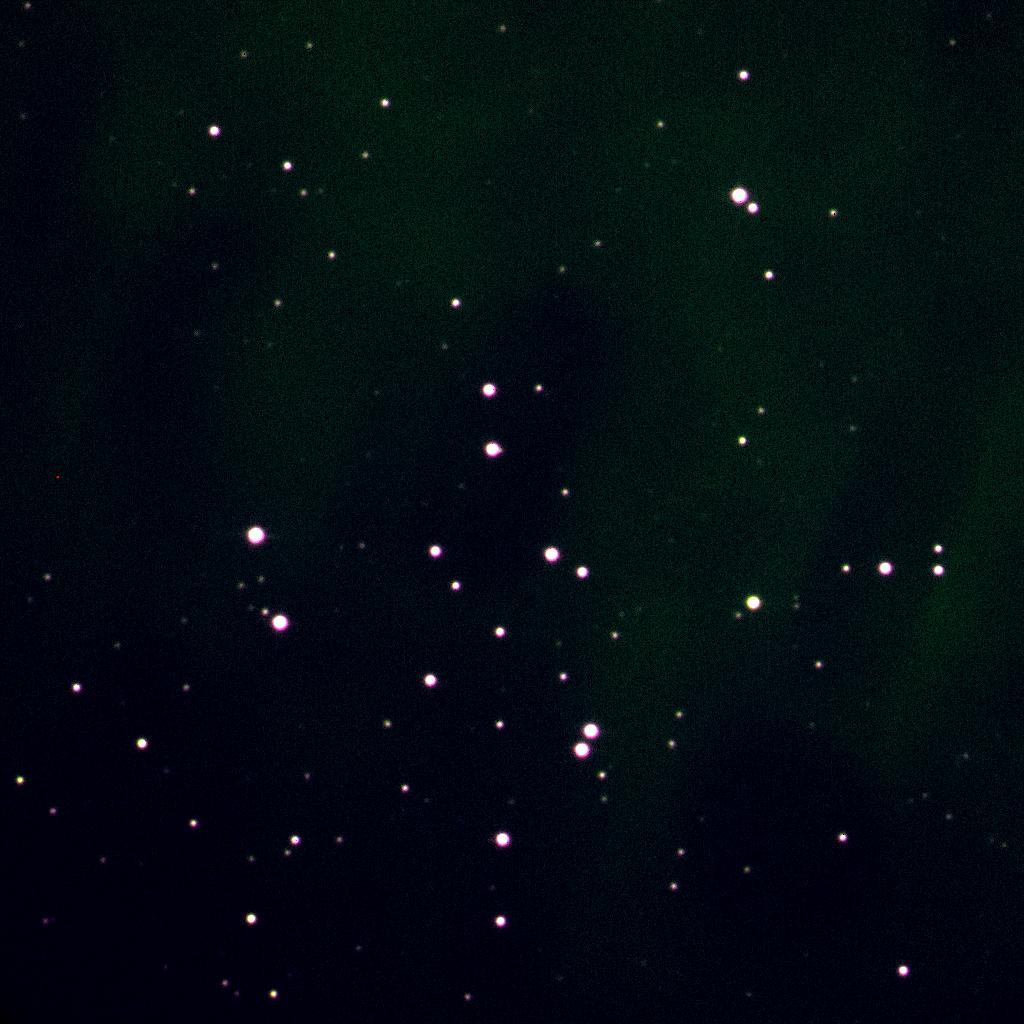
\includegraphics[width=0.8\textwidth,angle=-90]{Cluster/RGB_M34.png}
    \caption{RGB composite image of cluster M34 compiled from Johnson R,I and V filters taken with the Innsbruck $\SI{60}{\cm}$ telescope.}
    \label{fig:title} 
\end{figure}

\begin{abstract}
The Innsbruck $\SI{60}{\cm}$ observatory provides an excellent opportunity for students to familiarize themselves with the operation, data acquisition and data reduction processes used in astronomy. In this work, we present our results of working with the instrument and the data acquired in the \ldq Teleskoppraktikum\rdq during the winter semester 2018/19 at the University of Innsbruck.

In particular we describe the instrument calibration, the data reduction for imaging and spectroscopy and the results of our observations of open clusters, a comet, as well as stellar spectra. Furthermore, we touch on the subject of lucky imaging and use catalog data to investigate the status of open cluster candidates. 
\end{abstract}

\pagebreak
\tableofcontents

\pagebreak
\section{Introduction}

Learning how to operate a telescope and how to work with the data one can derive from observations of the sky is the primary goal of the \ldq Teleskoppraktikum\rdq. The $\SI{60}{\cm}$ Cassegrain telescope at the observatory of the University of Innsbruck and the instruments available there, are the tools used to achieve our first real foray into astronomy. This report takes us from the utter excitement during our first observations to the results accomplished by weeks of team work and individual efforts via a slight detour to our first setbacks and our learning process. 

The Innsbruck $\SI{60}{\cm}$ telescope is located  atop the Victor Franz Hess building at the Technik campus of the University of Innsbruck ($00$h$45$m$22.20$s, $\SI{47}{\degree} \SI{15}{\arcmin}\SI{51.19}{\arcsec}$, $\SI{580}{\m}$ above sea level). It is the only ground based observatory used for our work during the \ldq Teleskoppraktikum\rdq.

The course takes place from late October 2018 to the end of February 2019, where the first few weeks are used for lectures on the basics of astronomy, telescope calibration and image reduction using tools like IRAF. From December on, we start with the actual observations, finishing in late January. Afterwards we work with the gathered data using a multitude of software tools and approaches to familiarize ourselves with the processes that are used regularly in astronomy.

Altogether six days are used for observations, of which two are used for gathering calibration data, one for spectroscopy using an Echelle spectrograph one for both imaging and spectroscopy using a Littrow spectrograph and two specifically for imaging alone. Additionally, some data is taken by the lecturers during the semester and is provided to us and the other students. 

This report showcases all the steps of our work during the \ldq Teleskoppraktikum\rdq, starting with the calibration of the setup in section~\ref{sec:calibration} and an overview of the reduction procedure in section~\ref{sec:reduction}. Where the first one explains the determination of the optimal CCD temperature and pixel binning for the different cameras used and the second one the reduction of the various imaging data taken during the observation runs during the course. 

Next, in section~\ref{sec:imaging}, we describe the procedure and hardships we encounter while using the telescope for imaging purposes. In particular the imaging of a comet close to Earth and open galactic clusters is explained in this section. We focus on the procedure of extracting the position and brightness information of stars from an image, as well as the creation of Hertzsprung-Russell diagrams from images in several filters and the identification of probable members to the imaged clusters (and cluster candidates respectively) with data taken by the ESA spacecraft/mission \textit{Gaia}. 

In this section we additionally introduce lucky imaging as a method to counteract the influence of Earth's atmosphere on the image quality by reviewing the results of stacked images of Moon observations with a lucky imaging camera. 

Finally, in section~\ref{sec:spectrum}, the spectra taken during the course are analyzed and the procedure of taking a spectrum and reducing the data received, is explained with the aid of the spectra of two bright and well studied stars Vega and Deneb.

\section{Calibration}\label{sec:calibration}
In this first step we perform a calibration on camera 1 and 2, to find the optimal working temperatures for the cameras. We take multiple images for each temperature step, reducing statistical outliers and giving us a clearer picture on how the camera performs. We take images for all temperatures with a binning of 1 and 2.
\subsection{Bias calibration}\label{sec:bias_calib}
\subsubsection{Camera 1}
For camera 1 we get an initial set of 10 images for each temperature from $\SI{-5}{\celsius}$ to $\SI{-40}{\celsius}$ in $\SI{5}{\celsius}$ steps, with binning 1 and 2. These images are then combined, with outliers being clipped from the averaging process, giving us only real bias values. We then generate a master bias file for each temperature, that is then used for the dark calibration. Figure \ref{fig:Bias_old_b_1_calib} and figure \ref{fig:Bias_old_b_2_calib} show the resulting CCD images for binning 1 and 2.
\begin{figure}[H]
    \centering
    \includegraphics[width=\linewidth]{calibration&reduction/bias_b_1.pdf}
    \caption{Bias images for camera 1 for different temperatures as noted in the titles with binning of 1. The biases show stronger structures, the lower the temperature is set.}
    \label{fig:Bias_old_b_1_calib}
\end{figure}
Through visual inspection of these images, one can clearly see the emergence of a regular, horizontal pattern in the biases for lower temperatures. Clearly these lower temperatures are therefore not useable for proper imaging, as these will deform images and distort them. A clear reason for these vertical regularities was not found up to the point of writing this report. It is suspected that the shared power supply for the cameras is maybe to blame for this behaviour. We also can see some vertical regularities, from the first temperature step on. These are probably features of the CCD itself, and need to be noted and known in the further analysis. Looking at the behaviour of camera 1 with a binning of 2, this behaviour is persistent and even more expressed, again especially for lower temperatures. Figure \ref{fig:Bias_old_b_2_calib} shows the CCD images for binning 2. Because of the clear worsening in the behaviour of the camera we decide to only use a binning of 1 from here on out.
\begin{figure}[H]
    \centering
    \includegraphics[width=\linewidth]{calibration&reduction/bias_b_2_c_1.pdf}
    \caption{Same as figure \ref{fig:Bias_old_b_1_calib} but with binning 2. A even more distinct expression of vertical and horizontal structures is present for this setting.}
    \label{fig:Bias_old_b_2_calib}
\end{figure}
This effect in the biases leads us to the idea of disabling other cameras while taking images with the imager. We again take new biases for this camera, leading to the result shown in figure \ref{fig:Bias_new_b_1_calib}.
\begin{figure}[H]
    \centering
    \includegraphics[width=\linewidth]{calibration&reduction/bias.pdf}
    \caption{Bias images for camera 1 with reduced load on the power supply with binning 1. Vertical structures are still visible, horizontal structures begin to appear at $\SI{-35}{\celsius}$.}
    \label{fig:Bias_new_b_1_calib}
\end{figure}
This leads to an improved image in the biases. The horizontal lines at $\SI{-35}{\celsius}$ are weaker than the ones done in the first batch, yet still visible, so the problem is not totally solved using this solution. All further analysis for camera 1 takes place using this new batch of images. Looking at the distributions of the pixel values in figure \ref{fig:Bias_calib_hist}, we can see this behaviour as well. For the lowest temperature at $\SI{-35}{\celsius}$ we can see some slight edging out in the distribution, while for the lower ones this behaviour seems to be mostly nonexistent. We find clear gaussian distributions for the pixel values. This is to be expected, as the process that creates the bias should lead to normally distributed pixel values.
\begin{figure}[H]
    \centering
    \includegraphics[width=\linewidth]{calibration&reduction/bias_hist.pdf}
    \caption{Distribution of pixel values for the different temperatures. The y axis for all plots is logarithmically plotted to better see the features of the dataset.}
    \label{fig:Bias_calib_hist}
\end{figure}

\subsubsection{Camera 2}
While we use camera 1 fairly extensively throughout this work, the second camera was rarely used. We therefore lack some practical experience using this camera. Similarly to camera 1 we get a batch of biases and darks to perform a calibration on the camera. We again use multiple bias images for a temperature range between $\SI{0}{\celsius}$ and $\SI{-45}{\celsius}$ for binning 1 and 2.\newline
Visual inspection of the biases shows the emergence of vertical patterns on the CCD as seen in figure \ref{fig:Bias_old_c_2_calib}. By looking at the distribution of pixel values, as seen in figure \ref{fig:Bias_c2_b_1_hist}, the structural behaviour of this is clearly discernible at $\SI{-45}{\celsius}$. Looking at these distributions, a temperature in the middle ranges is preferable, as these seem to reproduce the best behaviour of camera 2.\newline
\begin{figure}[H]
    \centering
    \includegraphics[width=\linewidth]{calibration&reduction/bias_b_1_c_2.pdf}
    \caption{CCD images for camera 2 with binning 1, with different temperatures. We can clearly see more vertical structures on the CCD than on camera 1.}
    \label{fig:Bias_old_c_2_calib}
\end{figure}
\begin{figure}[H]
    \centering
    \includegraphics[width=\linewidth]{calibration&reduction/bias_hist_b_1_c_2.pdf}
    \caption{Distribution of pixel values for camera 2 with binning 1, with different temperatures. The pixel values are again logarithmically plotted. The best distributions for these temperatures can be found at $\SI{-20}{\celsius}$, $\SI{-30}{\celsius}$, $\SI{-35}{\celsius}$ and $\SI{-40}{\celsius}$. These show nice normal distributions for their pixel values. The rest has some deformities in their distributions, especially at $\SI{-45}{\celsius}$.}
    \label{fig:Bias_c2_b_1_hist}
\end{figure}
\begin{figure}[H]
    \centering
    \includegraphics[width=\linewidth]{calibration&reduction/bias_b_2_c_2.pdf}
    \caption{Same as figure \ref{fig:Bias_old_c_2_calib} but with a binning of 2. The structure of the CCDs does not resemble a bias anymore, but rather a very regular structural pattern, that shows vertical and diagonal structures.}
    \label{fig:Bias_old_c_2_calib_b_2}
\end{figure}
We also look at the behaviour of camera 2 with binning 2. This reproduces the by far worst result of all of them. We have a column like structure, that is overlapped by a diagonal structure at lower temperatures as seen in figure \ref{fig:Bias_old_c_2_calib_b_2}. Clearly there is a massive problem using this mode of the camera, making it useless for observations.
\subsection{Dark calibration}
With the analysis of the biases in different temperature ranges complete, we conclude that we will only use a binning of 1 for the further analysis of the dark current. To get a statistically good view on the dataset, we first combine a set of different dark images to one using an average combine again, similar to the bias procedure. We then remove the bias from the CCD, gathered through the analysis in section \ref{sec:bias_calib}. After this step the image is divided by the exposure time, as this is what we use as a master dark in a real observation. All pixel values after this process that are $<0$ are set to zero, to not introduce weird behaviour for the darks.\newline
We checked camera 1 with temperatures between $\SI{-5}{\celsius}$ and $\SI{-40}{\celsius}$. As expected the mean dark current decreases with decreasing temperature. Of course, through the structures visible in the bias frames (see section \ref{sec:bias_calib}) at lower temperatures, this also creates structures in the dark frame. Figure \ref{fig:Dark_c1_calib} shows the dark frames at different temperatures. A better view on the structure of the dark frames is visible through the distribution of pixel values. Figure \ref{fig:Dark_c1_calib_hist} shows the distribution of pixel values of the dark frames. Looking at these distributions, the optimal temperature for camera 1 would be $\SI{-30}{\celsius}$.
\begin{figure}[H]
    \centering
    \includegraphics[width=\linewidth]{calibration&reduction/dark_b_1.pdf}
    \caption{Dark frames for camera 1 with binning 1 for different temperatures. As expected, the dark current falls with falling temperatures on the CCD. Clear structures are visible on the CCD from $\SI{-35}{\celsius}$ on, making smaller temperatures not useful as a working temperature.}
    \label{fig:Dark_c1_calib}
\end{figure}
\begin{figure}[H]
    \centering
    \includegraphics[width=\linewidth]{calibration&reduction/dark_hist_b_1.pdf}
    \caption{Pixel value distribution for the dark current of camera 1 with a binning of 1. We see multiple peaks between $\SI{-15}{\celsius}$ to $\SI{-25}{\celsius}$. These peaks are probably due to the reduction of the images, where some pixels show a higher value for some pixels than would be expected and are not matched by the clipping process. They then vanish for lower temperatures.}
    \label{fig:Dark_c1_calib_hist}
\end{figure}
\begin{figure}[H]
    \centering
    \includegraphics[width=\linewidth]{calibration&reduction/dark_b_1_c_2.pdf}
    \caption{Same as figure \ref{fig:Dark_c1_calib} but for camera 2. Clearly there is a strange behaviour with this camera, as the image shows shadowing for the lower right part of the CCD, where a significantly higher dark current is visible. This structure is probably persistent through all temperatures, but only visible for these lower temperatures.}
    \label{fig:Dark_c2_calib}
\end{figure}
\begin{figure}[H]
    \centering
    \includegraphics[width=\linewidth]{calibration&reduction/dark_hist_b_1_c_2.pdf}
    \caption{Same as figure \ref{fig:Dark_c1_calib_hist} but for camera 2. We see a flattening out of the initial peak in the distribution for lower temperatures, giving us a broader dark current distribution. }
    \label{fig:Dark_c2_calib_hist}
\end{figure}
For camera 2 we performed the same analysis with temperatures between $\SI{0}{\celsius}$ and $\SI{-45}{\celsius}$. The behaviour of camera 2 is similar to camera 1. Its dark current decreases as the temperature decreases, as seen in figure \ref{fig:Dark_c2_calib_hist}. There is a significant shadowing effect on the CCD though from around $\SI{-35}{\celsius}$ onwards, as seen in figure \ref{fig:Dark_c2_calib}. This again leads us to the conclusion, that the best operating temperature of camera 2 is $\SI{-30}{\celsius}$.
\section{Reduction}\label{sec:reduction}
Reduction of observed images with a modern telescope (imaging on a CCD) is a very integral part for the quality of the dataset. To perform this reduction, multiple steps need to be taken, as will be explained in the following. We will first describe a theoretical reduction of a given dataset, continuing with a more practical approach as well as the technical details for the developed custom pipeline written in Python.
\subsection{Theoretical reduction}
For this theoretical reduction we assume a more or less ideal CCD with no hot pixels, no cosmic rays or other problems in the dataset. This is of course not the case for a real life CCD, yet this is the fundamental block we will work with.\newline
The first step in the reduction is the capturing of a bias image. This is usually done by simply reading out the CCD without opening the shutter of the camera. In theory, this is simply a constant value caused by the constant voltage applied to the detector itself. We call this value $\sigma_\text{b}$. The next step consists of taking a dark frame image. This gives us the dark current $\sigma_\text{d}$ in the dataset, representing the thermal electrons that are read out from the CCD through the ambient temperature of the chip. This effect is reduced to a minimum through the cooling of the chip (see section \ref{sec:calibration}). To compute the dark frame image, we expose the chip with the shutter closed for a given time (we usually choose around $\SI{30}{s}$). In the reduction, we then subtract the bias from the dark current and divide the image through its exposure time. The dark current is therefore
\begin{equation}
    \sigma_\text{d} = (\sigma_\text{d}' -\sigma_\text{b})/t_\text{exposure}
\end{equation}
The last part that is needed is the so called flat field $\sigma_\text{f}$. Pixels on a CCD are not perfectly equally sensitive to exposure. There might be some structure in the CCD, stemming from the production of the chip or the readout electronics might have an effect. This means that any image exposed on the chip will not be uniformly well lit out, which is corrected using the flat field. To get a flat field image, multiple techniques are possible. For example, we could use an evenly illuminated white flat surface which is then exposed on the CCD. This of course is a bit difficult, as the focal length of the telescope might not be perfectly aligned with such an object. We therefore chose to perform the second method for most of our later observations. For this, one starts the observations a bit earlier in twilight. We then take an image of the twilight in the horizon, giving us a decent enough lit out flat field of the CCD. To get the final flat field, we take this image and subtract the master bias and dark multiplied by the exposure time. This gives us
\begin{equation}
    \sigma_\text{f}' = (\sigma_\text{f}'' -\sigma_\text{b} -\sigma_\text{d}*t_\text{exposure})
\end{equation}
This, of course, is not enough, as we want to multiply the flat field with the observations of our target. We therefore divide the flat field through the median.
\begin{equation}
    \sigma_\text{f} = \sigma_\text{f}'/\widetilde{\sigma_\text{f}'} 
\end{equation}
The median is used, because we don't want to massively change the true pixel values of the dataset in our observations. Using the maximum could lead to non sensical pixel values in the CCD.\newline
Finally, our observations can be reduced using these values. To reduce an observation, one subtracts the bias and dark current from the image and divides the image through the flat field. So to get real observational data we need to perform
\begin{equation}
    \text{IMG} = (\text{IMG}' -\sigma_\text{b} -\sigma_\text{d}*t_\text{exposure})/\sigma_\text{f}
\end{equation}
which gives us the reduced CCD data.
\subsection{Practical application}
In practice, the CCD is of course not perfect. There are therefore multiple other steps that need to be taken to ensure a well enough reduction of the data set. To reduce statistical uncertainty in the data, we take multiple bias frames and dark frames. We then remove cosmics and outliers through the median and only accept values within a given range. These values are then averaged, giving us a good idea of the bias and dark frames. \newline
In principle, the twilight flat fields are a good method to get decent flats for the CCD. But we also need to take multiple images here, as even in twilight, stars are clearly visible in the image. We move the telescope slightly before each flat field, and perform the same combination method used for darks and bias images. We also need to create a flat field for every filter that is used in the observation, as these filters can have a significant impact on the image. It should be also noted, that temperatures need to be constant for this whole process, which is due to the different behaviour at different temperatures in the CCD.\newline
This whole process was automated using a custom pipeline written in Python. This pipeline reads the images from a given folder, and given that this folder contains bias, dark and flat field frames, it computes a master dark, master bias and master flat for all filters in this folder and reduces all light frames. The information for each file is read out through the fits header of the file. We first combine the biases using an average combine method, and generate a master bias for a given data set. It then creates the dark by subtracting the master bias from every single dark frame, and combines them using the average combine technique. The flat images are created for every single filter and this is applied to the light frames taken for our targets.

\section{Imaging}\label{sec:imaging}

Imaging is the main objective of the second half of our \ldq Teleskoppraktikum\rdq. The primary goal is to take images of several open clusters and possible candidates in different filters. From these images color magnitude diagrams are created. Additionally, one can search for proper motion and distance information for the imaged stars in catalogues and use this information and the color of the stars to check their membership to the given open cluster or open cluster candidate. If these parameters can be gathered for enough stars, one can conclude whether the imaged cluster candidate is in fact an open cluster. Furthermore one can also get information on the size of the clusters with this technique. 

In addition to the imaging of clusters and cluster candidates we image comet 46P/Wirtanen as a target of opportunity. We also use the lucky imaging technique to image the moon in higher quality than would be possible with a classic imager.

\subsection{Imaging of a comet}

On December $13^\text{th}$ the weather conditions allow us to try to image comet 46P/Wirtanen, which had its closest approach to Earth around that time. The seeing is mediocre during the observation and the observation direction right towards the city does not help the image quality either. Furthermore, the behaviour of the imaging camera (Camera 1) was not entirely understood at the time, which challenges us greatly during the reconstruction of the images.
The comet is seen over Innsbruck at a right ascension of $\num{03}\,$h$\,\num{37}\,$m$\,\num{20}\,$s and a declination of $\SI{11}{\degree} \num{45}'\num{26}"$ at around 18:00 CET. Therefore the observations are done at a very low angle above the city which explains the high background noise in all images taken of 46P.

Searching for 46P/Wirtanen on the sky is done by interpolating between data points given in an ephemeris table \parencite{wirtanen} of the comet and manually pointing the telescope to the calculated coordinates. After finding the comet, the telescope position has to be readjusted occasionally as the comet is of course moving with respect to the reference frame of the stars which the telescope is tracking. Two $\SI{90}{\second}$ exposures of the comet are taken for each of the filters Johnson V, I and R. Furthermore, we take bias and dark frames as well as flat fields for all three filters. In addition, we then try to take a spectrum of the comet using camera 2 but unfortunately the comet is too faint and the conditions too bad to get usable data. The V, I and R images are also of mediocre quality, especially the V filter shows a very bad signal to background ratio. 

The reduction of the images is performed using our pipeline. Unfortunately the flat fields taken during the observation night are unusable as we did not complete the calibration of the camera, and chose a wrong temperature for the observation. To temporarily work around this and to be able to at least show a somewhat reduced image of 46P/Wirtanen we replace the flats with ones taken in January at a different temperature which of course only removes the influence of dust on the filter wheels but not the influence of the CCD at the time of observation. The three color composition of the \ldq reduced\rdq V,I and R images can be seen in figure ~\ref{fig:wirtanen}. Obviously this is not a true RGB composition but rather a stack of the individual colorized images but a true composition is unfortunately rather bad, as one can see in figure~\ref{fig:wirtanen_start} which also shows the original unmatched V, I and R channels overlaid. These are fairly nice to look at, but are of little scientific value.

\begin{figure}[H]
    \centering
    \begin{minipage}{1.\textwidth}
    \centering
       \includegraphics[width=0.6\textwidth]{Comet/composite_no_smooth.pdf}
    \end{minipage}
       \begin{minipage}{1.\textwidth}
       \centering
       \includegraphics[width=0.6\textwidth]{Comet/composite_smooth.pdf}
    \end{minipage}
 
    \caption{Comet 46P/Wirtanen in a three color composite from Johnson I,V and R images taken on 2018-12-13 with the Innsbruck 60cm telescope. The lower image was smoothed by convoluting a 5 by 5 pixel 2D-Gaussian filter of order 0. The stars in the background appear once in every colour as the comet moved significantly between each exposure, while the telescope was tracking the stars. Due to the movement of the comet during the exposures the position match up for the composition is not perfect.}
    \label{fig:wirtanen}
\end{figure}

\begin{figure}[H]
    \centering
    \begin{minipage}{1.\textwidth}
        \centering
       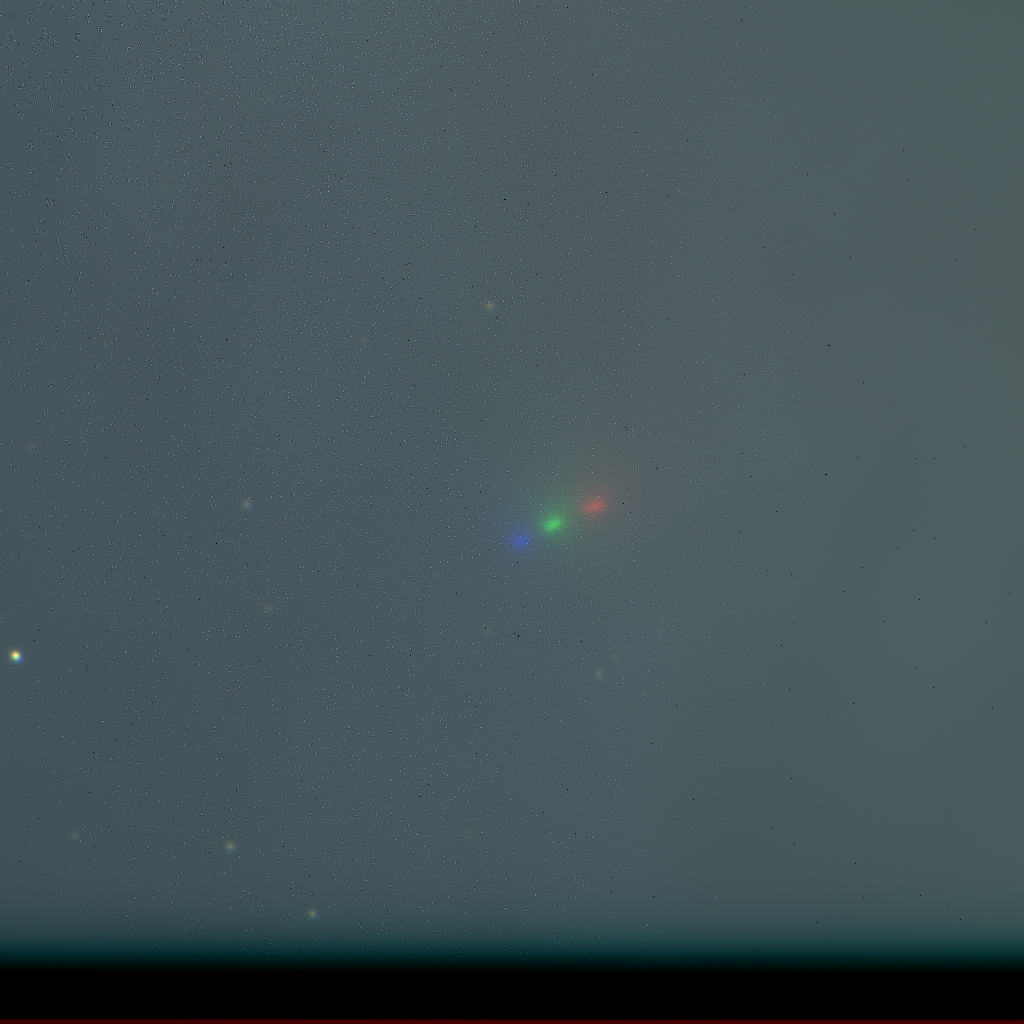
\includegraphics[width=0.6\textwidth]{Comet/RGB_comet_unmatched.png}
    \end{minipage}
       \begin{minipage}{1.\textwidth}
       \centering
       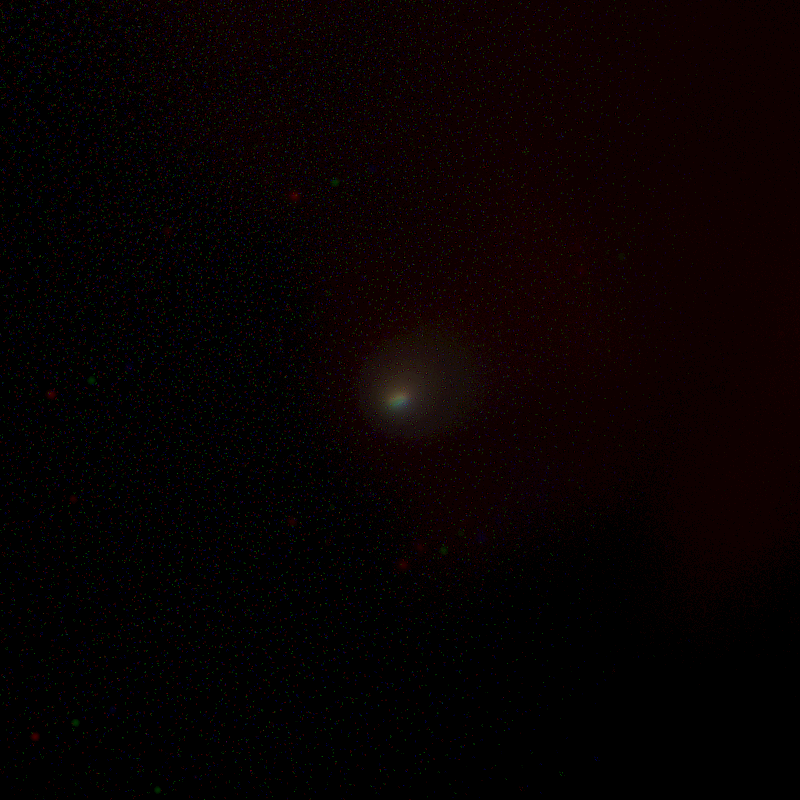
\includegraphics[width=0.6\textwidth]{Comet/comet_rgb_snow.png}
    \end{minipage}

 
    \caption{Top: initial unmatched image of 46P/Wirtanen from the three filters. Bottom: Highly edited RGB composition matched on the comet position. A smoothed version was produced but the comet is very faint and therefore hardly visible.}
    \label{fig:wirtanen_start}
\end{figure}

From the offset of the comet in different images and the known times at which the images are taken one can try to reconstruct the velocity of the comet across the sky. When doing this we encounter the problem that our imaging software does not include the telescope pointing position in the FITS header which means that we have no reference which pixel in the image corresponds to which position on the sky. Adding this information later is complicated as there are distortions on the projected image from the telescope optics and the spherical sky which rules out a linear conversion from identifying two stars and using their position to convert from pixels to right ascension and declination. 

Therefore, we use the Astrometry.net tool~\parencite{Astrometry} to find the world coordinate system (WCS) for our images. For this the tool uses a geometric hash code of four parameters which characterize the position on the sky of four stars independent of the image scale and rotation. The definition of these four parameters can be seen in figure~\ref{fig:quad}. Astrometry.net extracts the sources in the input image and builds a set of these parameters for every combination of four stars detected. These parameter sets are then compared with a database of index files which has been generated from several star catalogues like Tycho-2, 2Mass and USNO-B. If the parameters from the input image match the ones in the database, the position, rotation and scale of the world coordinate system is known and therefore the WCS is added to the header of the input .fits file. Surprisingly this nifty technique works, despite the image quality and low number of visible stars, for five of the six images of 46P/Wirtanen. 

\begin{figure}[H]
    \centering
    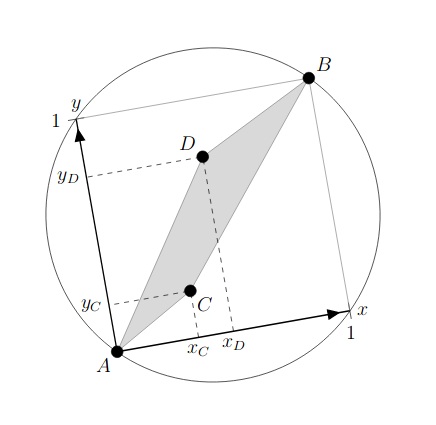
\includegraphics[width=0.5\textwidth]{Comet/quad.png}
    \caption{Definition of the geometric hash code parameters $x_C, x_D, y_C$ and $y_D$ used by the Astrometry.net tool for world coordinate system calculation. Image taken from \parencite{Astrometry}.}
    \label{fig:quad}
\end{figure}

As the output of Astrometry.net gives the star positions but no brightness of the objects we use SExtractor~\parencite{SExtractor} on all five images with a WCS to get the brightness in instrumental magnitudes and the position both in pixel and in right ascension and declination for the detected stars and the comet. From the time the image was taken (which is included in the .fits header) and the difference in the comet's position we can determine the proper motion of 46P/Wirtanen. Using this technique we determine an absolute value of the proper motion vector of $p_{46P} = \SI{2.2 \pm 1.3}{\arcsec \per \minute}$ which is significantly lower than the value expected from the ephemeris table of $\SI{9.83}{\arcsec \per \minute}$ given in ~\parencite{wirtanen}. Possible reasons for this include the difficult extraction of the actual comet position as the exposure time is long enough for the comet to smear out in the image and the comet potentially being actually slower than expected.

\subsection{Imaging of open clusters}

We image open galactic clusters in order to create Hertzsprung-Russell (HR) diagrams and study the membership of the individual stars to the clusters. The studied objects are M34, Teutsch 55, C0001+557 (also known as Stock 19) and Patchick 78. While the first one, M34, is very well studied the other three are not. All of them are located on the northern sky and therefore readily observable from Innsbruck. Two observation nights on the $16^{\text{th}}$ and $22^{\text{nd}}$ of January 2019 are used to observe these objects. M34 and Patchick 78 are only observed during the first night, Stock 19  only during the second night and Teutsch55 during both nights. While observing Patchick 78 it quickly becomes clear that the members of this cluster are mostly too faint and therefore observations of it are stopped immediately in favor of Teutsch 55. Prolonging the exposure time for Patchick 78 is not possible as the images become too background dominated.

The images of the clusters are reduced using our reduction pipeline and then given a world coordinate system using the Astrometry.net tool. As the observation conditions during the two nights in January were much better than the one where 46P/Wirtanen was imaged in December, all images have a unique solution for their world coordinate system. This leads to the possibility of automatically searching the \textit{Gaia DR2} catalogue with the coordinates of all cluster stars derived from the WCS. For this automatic \textit{Gaia} query we use the Python package astroquery~\parencite{astroquery}. This procedure will be discussed in more detail in section~\ref{sec:Gaia}. A RGB composite image of one of the studied clusters can be seen in figure~\ref{fig:title} on the title page.

\subsubsection{Hertzsprung-Russell diagrams}

As we image the open clusters in four different filters we can create HR diagrams in the form of color-magnitude-diagrams. The lack of magnitude calibration/zero point for our telescope does not affect these as only differences of colors are relevant, which of course do not depend on the absolute scale of the brightness of the stars. To create the observational HR diagrams we extract the sources from four images in the different filters (Johnson V,I,R,B) using SExtractor~\parencite{SExtractor}. This gives us the extracted position and brightness of the imaged stars in every filter. Some stars are only visible in part of the images, as they are for example brighter in the blue and therefore fainter or even not visible in the redder filters. This, of course, has to be taken into account when creating HR-diagrams. Therefore we only use extracted stars which can be found in all filters on the same pixel position in the image (with a tolerance of $\SI{\pm 3}{\pixel}$). For this procedure images with an exposure time of several hundred seconds (depending on the filter) are used, in order to make sure that even faint sources are included in the study.

The number of sources extracted varies greatly with the input parameters of the source extraction process. Primarily the threshold above which a pixel is counted as non background and the minimum area of joint pixels above this threshold indicate whether a bright spot in the image is a star or not. Furthermore, the seeing can be (in part) compensated by allowing for objects with a rather high FWHM to be still considered stars and not extended objects. The level of the background can also be adjusted individually for each filter. If the parameters chosen are too constricting no stars are extracted from the image, however if they are not constricting enough, large areas of the background are detected as extended sources. Both of which is unwanted and therefore compensated by redoing the analysis with different input parameters. 

SExtractor has hundreds of possible return values of which we are interested in mainly three: the position of the extracted source in pixels (for x and y direction respectively) and the brightness of the source in uncalibrated instrumental magnitudes. The position is used for matching the stars between different filters and the brightness is then used for the HR-diagrams. These are simple plots of the difference of brightness in two filters versus the brightness in one of the filters, for example B-V versus V. The resulting diagrams are shown in figure~\ref{fig:HR} for the clusters M34, Teutsch 55 and Stock 19. Especially the one for M34 clearly shows the main sequence as expected. 

\begin{figure}[H]
    \centering
    \includegraphics[width=1.\textwidth]{HR_diagrams/HR_M34.pdf}
    \includegraphics[width=1.\textwidth]{HR_diagrams/HR_Teutsch55.pdf}
    \includegraphics[width=1.\textwidth]{HR_diagrams/HR_Stock19.pdf}
    \caption{Hertzsprung Russell diagrams from the four filters Johnson B,V,I and R for the stars in the image frams for the clusters M34 (top), Teutsch 55 (middle) and Stock19 (bottom).}
    \label{fig:HR}
\end{figure}

\subsubsection{Determination of cluster membership using Gaia}
\label{sec:Gaia}

The automatic query search for \textit{Gaia DR2} entries for the extracted stars is done using the Python/astropy package astroquery~\parencite{astroquery}. The tool searches the online \textit{Gaia DR2} catalog for the positions extracted by SExtractor for the given clusters. The query returns the complete \textit{Gaia}entry of the star which includes the source ID, position, proper motion, parallax, and other parameters depending on which were measured by Gaia. 

As the \textit{Gaia DR2} catalog has a lot of entries often times the query returns more than one \textit{Gaia}entry for an extracted position. In this case we ignore the star at the extracted position for the further analysis as it is often not possible to tell which of the entries is the correct one. In very rare cases we can not find a \textit{Gaia}entry for an extracted position which also leads to us skipping the position. 

The whole process is done only for the sources which are present in all four filters for each cluster candidate as we want to be able to use the color of the stars as an indicator of their cluster membership. Unfortunately this also means that there are very little sources for which we have a \textit{Gaia}entry and a color, especially for Teutsch 55 and Stock 19 (under 20 stars in both cases). Therefore we decide to not go further into this automated search but rather use the old fashioned way of looking at the images, numbering the stars, looking up their \textit{Gaia}ID and finding their parameters this way (i.e. using a human SExtractor). %Wollt i unbedingt erwähnen %LOL... fantastisch!
Of course this unfortunately removes the color information as the reverse process of looking up the stars in all our images is tedious and error prone. Therefore we decide to solely rely on proper motion and distance information for determining cluster membership. The manual method proves to be the vastly superior one, although the immense time consumption is usually very hard to justify.  

So in order to determine the membership of the imaged stars to a cluster, we followed the following procedure shown in the flowchart (figure \ref{fig:flowchart}). It and the followed analysis will be quickly summarized in the following:

\begin{enumerate}
\item We take an observation and make as many light sources visible as possible. It turned out that the red filter was in every case the filter with the most sources visible; blue was always the worst one.
\item Check if the light source of our observation is also visible in the Digitized Sky Survey (DSS2) on \textit{Aladin}\cite{Boch2014}.
\item If it is visible in both images, put a number on this star (cf. \ref{fig:obsM34_num} and \ref{fig:DSS2M34_num}).
\item Use \textit{Aladin} in order to find the corresponding \textit{Gaia DR2 source IDs} (SIDs) to those stars. However, if there were multiple sources very close to each other, this source was not used.
\item Import those extracted \textit{SID}s in the \textit{ESA Gaia archive}\footnote{\url{https://gea.esac.esa.int/archive/}} (\cite{Gaia2016}, \cite{Gaia2018}).
\item Extract valuable properties like: right ascension, declination, the proper motion in those directions, the \textit{Gaia}magnitude, the parallax and the errors of those values.
\item Using the position and magnitude of every light source we can reconstruct our observation image (cf. \ref{fig:M34_pm}). The proper motion can also be illustrated by arrows originating from the corresponding star.
\item Now we can take a look at the distribution of distances and proper motions using a histogram (cf. \ref{fig:M34_histogram_all}). We can exclude outliers in distance and the proper motions using an iterative three sigma clipping procedure. Meaning, we removed all stars outside the three sigma regime with respect to the median. This eliminated outliers with high or low distances or proper motions. This clipping was repeated until nothing was 'clipable' anymore. Notice that having the right distance is not enough; you also need the right proper motion. Using a Gaussian fit on the remaining stars, which will be called cluster members (CMs) from here on, gives us our guess for the distance and the mean proper motion of this cluster.
\item As an independent check we also have a look at the radial velocities of our CMs (cf. \ref{fig:M34_histogram_RV}). Our CMs should not be seen as outliers here.
\item As additional information, we also provide a histogram of the magnitudes of our extracted sources and our CMs (cf. \ref{fig:M34_histogram_mags}).
\item Followed by a new reconstruction of our observation image just containing the CMs and their proper motions (cf. \ref{fig:M34_pm_mask}). 
\item Finally, we show the distribution of the proper motions together with the mean and standard deviation in the proper motions of the cluster extracted from the gaussian fit (cf. \ref{fig:M34_pm_scatter_sigma}).
\end{enumerate}

\begin{figure}[H]
  \centering
    \includegraphics[trim={0 16.6cm 0 0.5cm},clip, width=1\textwidth]{Cluster/flowchart.pdf}
  \caption{This flowchart summarizes the procedure, which was used in order to extract the sources from our observations.}
  \label{fig:flowchart}
\end{figure}

\begin{table}[H]
\centering
\caption{\textbf{Num. stars}: Number of extracted sources from our observations for every cluster. \textbf{Not used}: Number of sources not used, because the existence of two or more \textit{Gaia DR2} entries very close by. \textbf{Two parameter sol.}: Some stars are lacking the full five parameter solution (position on the sky in RA and Dec, proper motions and parallax), but only have a two parameter sol. (RA and Dec). Those stars were not used in the following analysis. \textbf{Neg. parallax}: Stars with negative parallaxes were also excluded from the analysis. Those stars also typically have big uncertainties in their parallax or proper motions. \textbf{Analysed stars}: The final number of analyzed stars. \textbf{RV stars}: Number of extracted sources with a radial velocity value. It was only available for a small number of stars.}
\label{tab:sources}
\begin{tabular}{l|c|c|c}
                   & M34       & Teutsch 55 & Stock 19  \\ \hline
Obs. date          & Jan. 16$^{\text{th}}$ & Jan. 16$^{\text{th}}$  & Jan. 22$^{\text{nd}}$ \\
Filter             & R         & R          & R         \\
Exposure time (s)  & 150       & 300        & 200       \\ \hline
Num. stars         & 195       & 191        & 208       \\
No \textit{Gaia DR2} entry  & 0         & 0          & 1         \\
Not used           & 6         & 5          & 0         \\
Two parameter sol. & 3         & 3          & 2         \\
Neg. parallax      & 2         & 0          & 2         \\
Analysed stars     & 185       & 184        & 203       \\
RV stars           & 28        & 33         & 37       
\end{tabular}
\end{table}

In the appendix (\ref{sec:appendix}) one finds the \textit{Gaia}data of all extracted stars - the cluster members, the non-cluster members and the stars, which were not analyzed. 

\paragraph{M34}

\begin{figure}[H]
  \centering
    \includegraphics[width=0.95\textwidth]{Cluster/obsM34_num.jpg}
  \caption{Our observation of M34 in the red filter with an exposure time of 150 seconds. The numbers are in correspondence with those in image \ref{fig:DSS2M34_num}.}
  \label{fig:obsM34_num}
\end{figure}

\begin{figure}[H]
  \centering
    \includegraphics[width=0.95\textwidth]{Cluster/DSS2M34_num.jpg}
  \caption{The negative of the observation of M34 by the DSS2. This picture was extracted from \textit{Aladin}. The numbers are in correspondence with those in image \ref{fig:obsM34_num}.}
  \label{fig:DSS2M34_num}
\end{figure}

\begin{figure}[H]
  \centering
    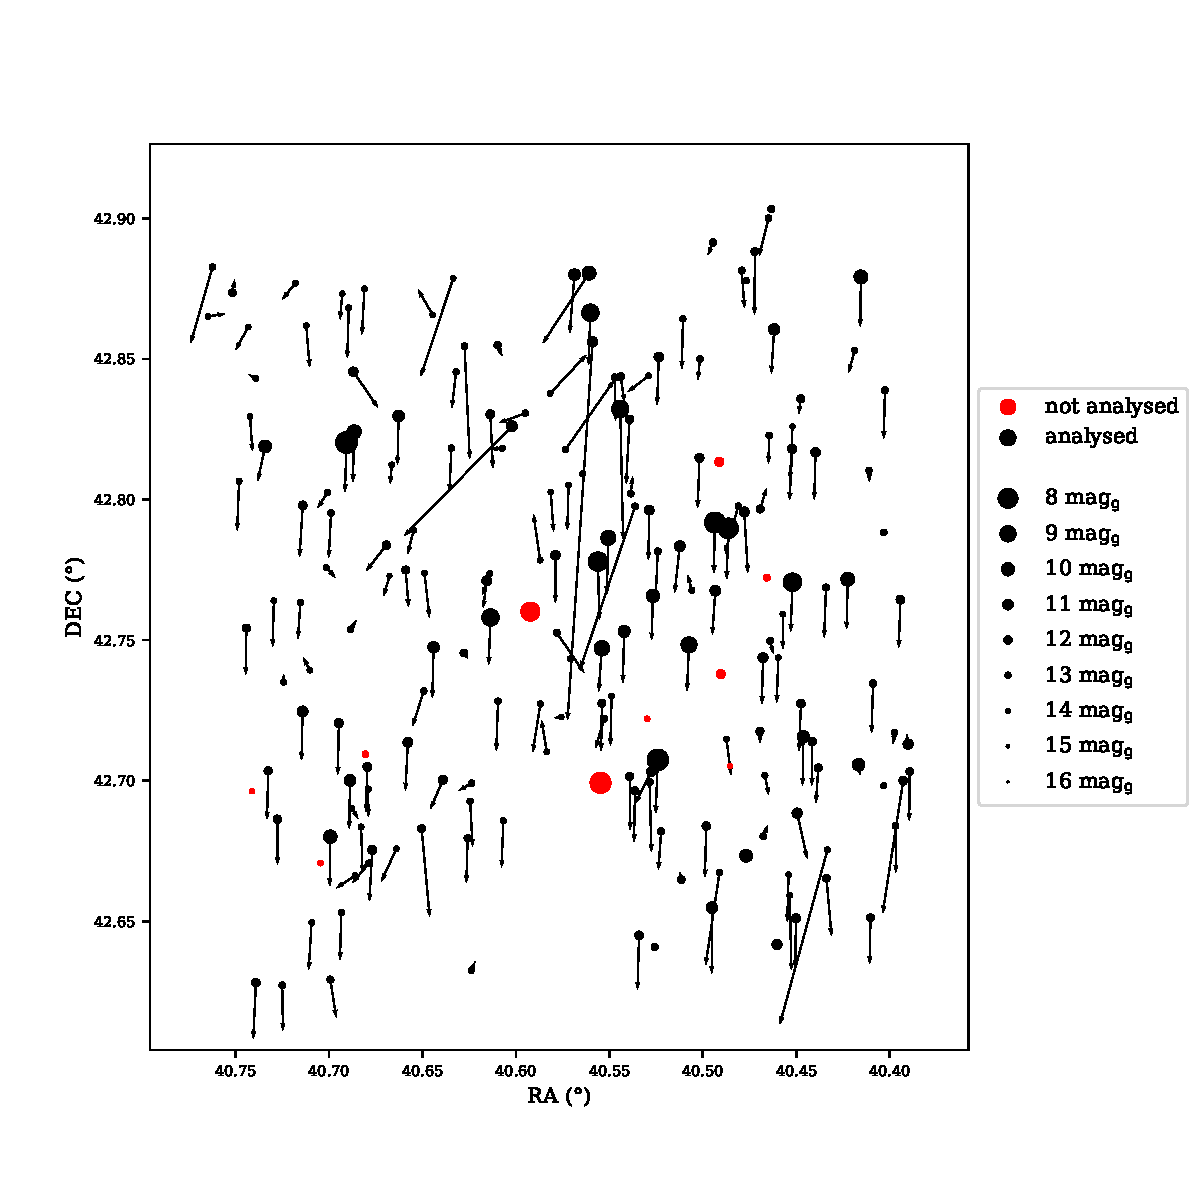
\includegraphics[trim={0 1.6cm 0 2.3cm},clip, width=0.95\textwidth]{Cluster/M34_pm.pdf}
  \caption{Every point is an extracted source. The size corresponds to the \textit{Gaia}magnitude. The arrows illustrate the direction of the proper motion. A star was for example not analysed if the proper motions were missing.}
  \label{fig:M34_pm}
\end{figure}

This figure \ref{fig:M34_pm} already illustrates that most stars are moving in the negative declination direction. One can also see some high proper motion stars.

\begin{figure}[H]
  \centering
    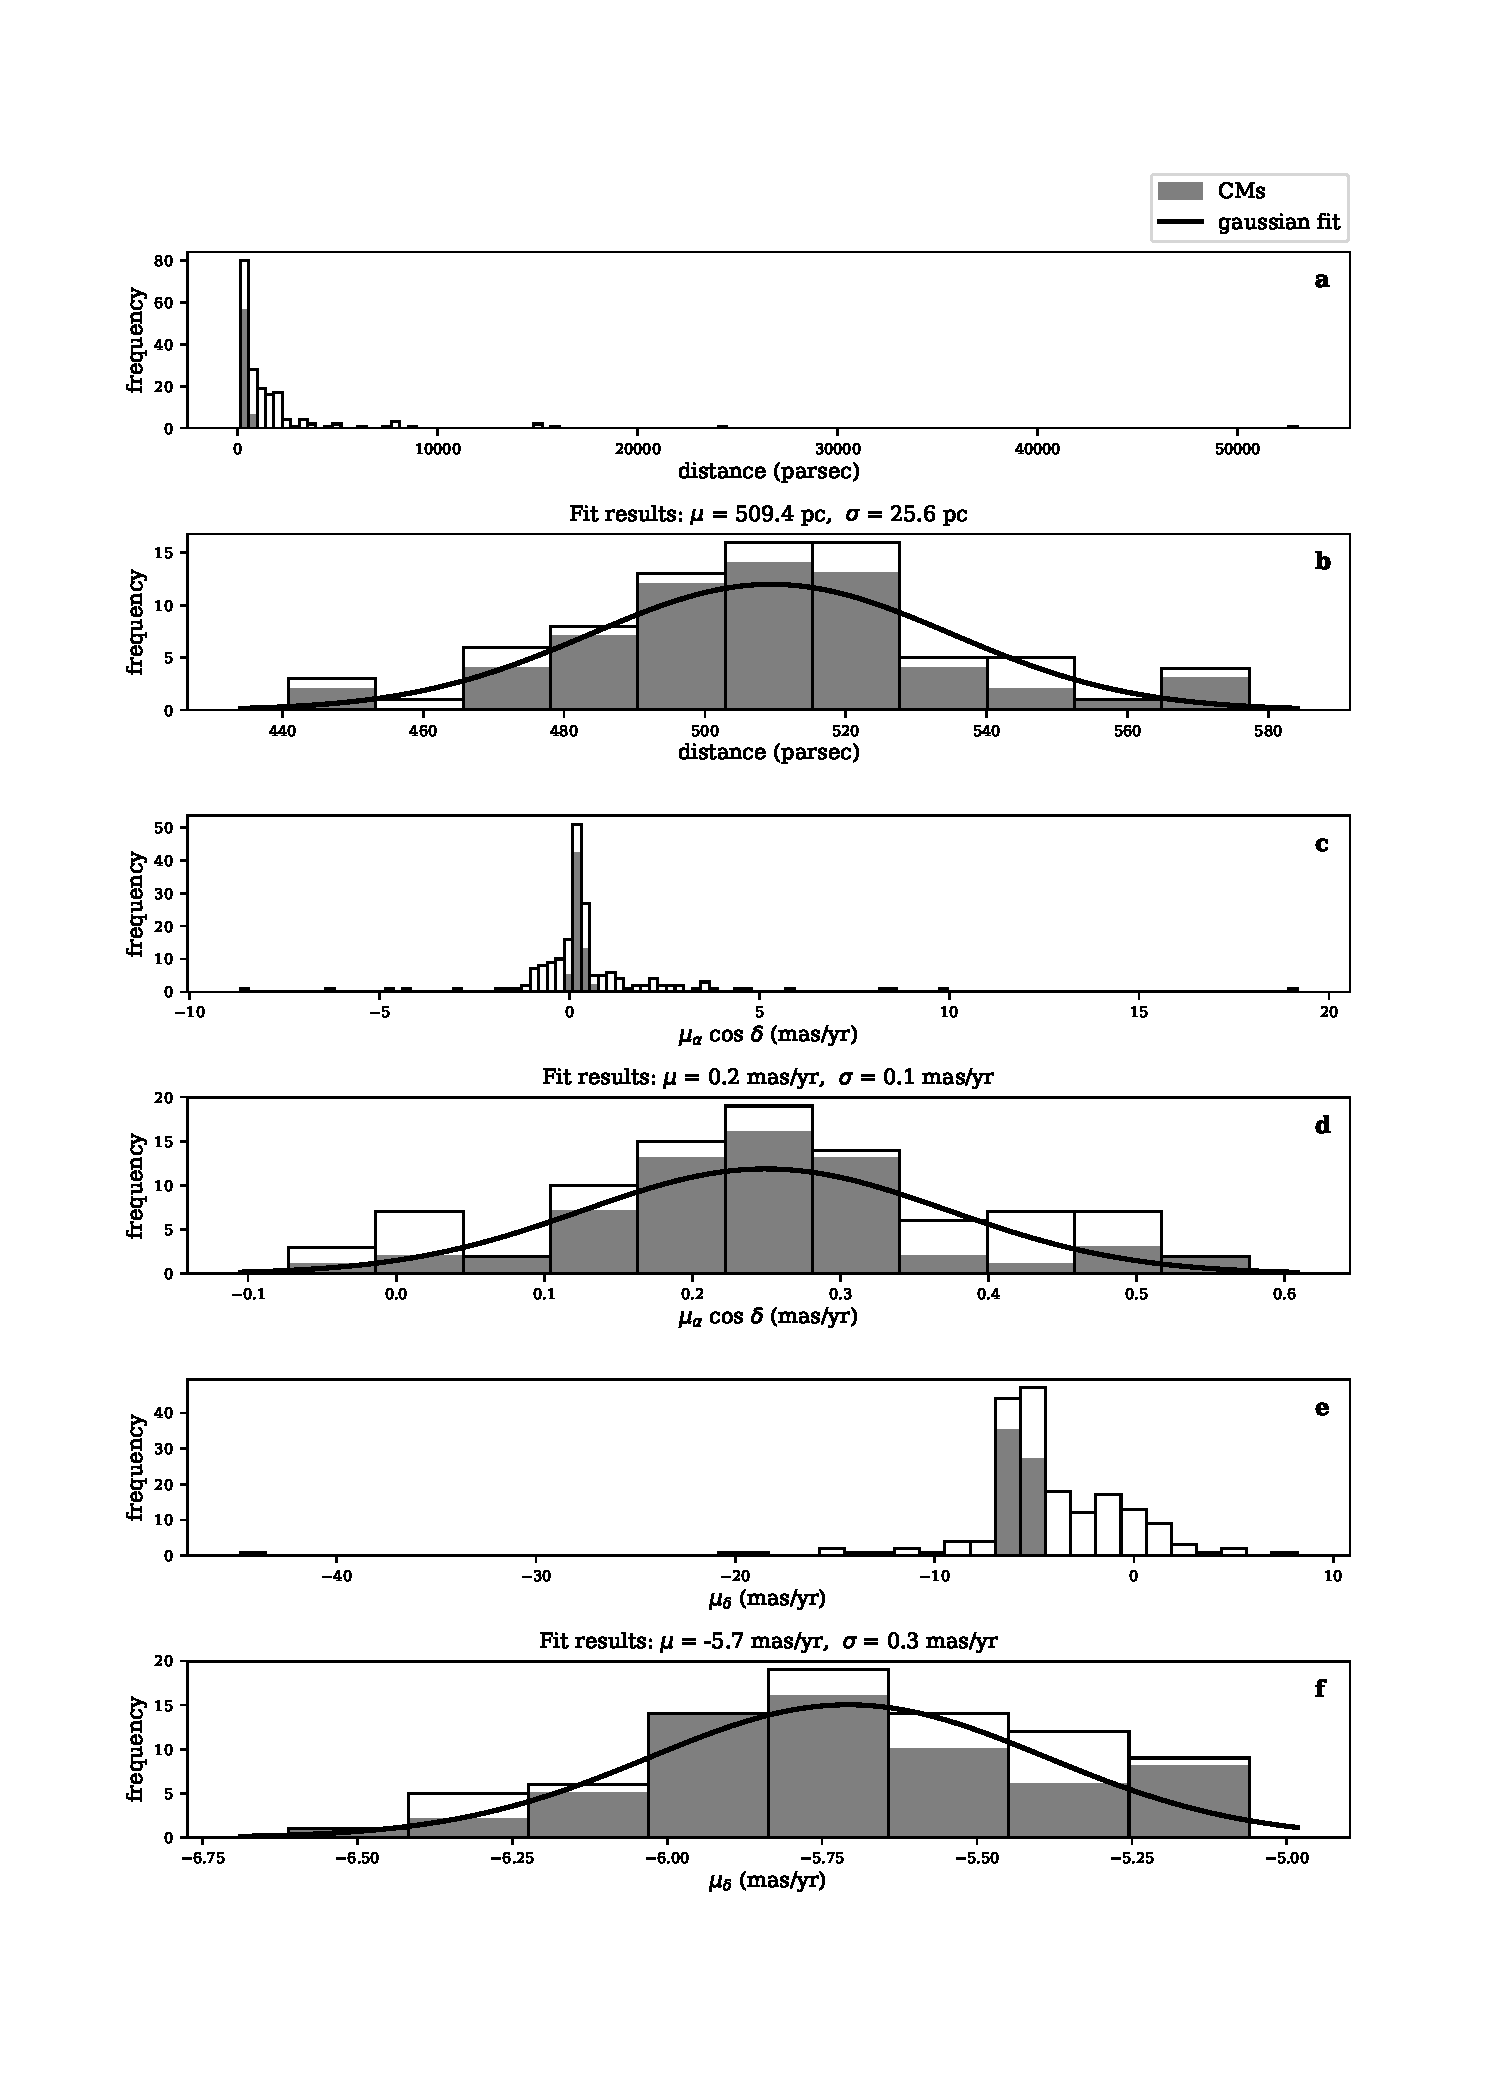
\includegraphics[trim={0 3.4cm 0 2.9cm},clip,width=0.95\textwidth]{Cluster/M34_histogram_all.pdf}
  \caption{Histogram of the analysed stars. In order to determine the Cluster members (CMs) an iterative sigma clipping procedure was applied (see point 8 in section \ref{sec:Gaia}). \textbf{a, c, e}: The distances and proper motions for all stars and the CMs (in gray). \textbf{b, d, f}: This zoom-in also includes a gaussian fit of the CMs. Above those plots the mean and standard deviation of this gaussian.}
  \label{fig:M34_histogram_all}
\end{figure}

\begin{figure}[H]
  \centering
    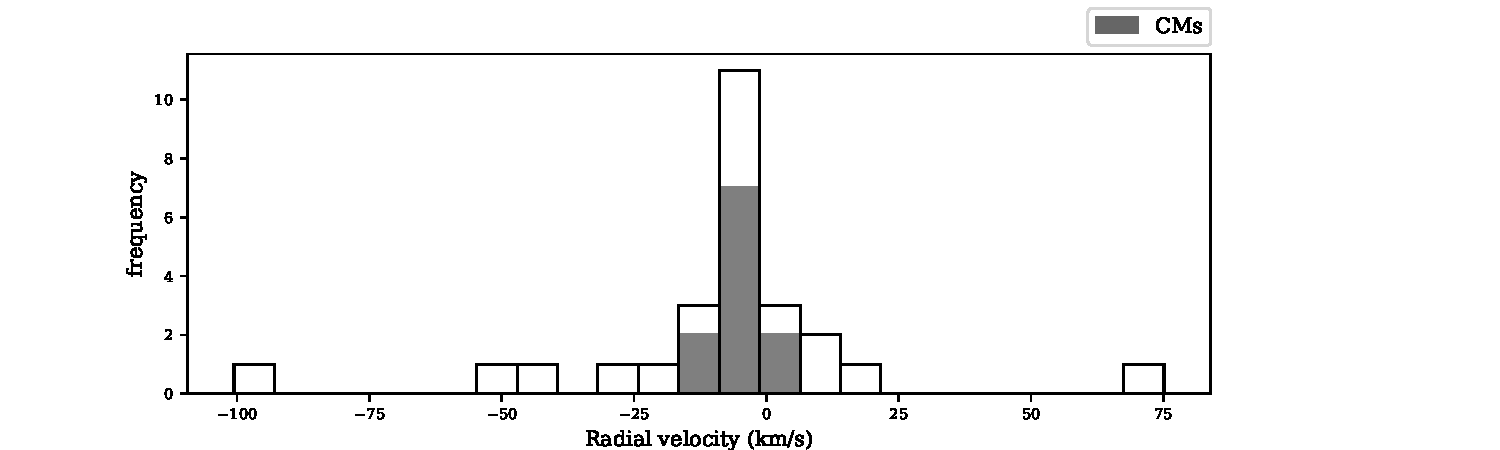
\includegraphics[trim={0 0 2cm 0},clip,width=0.95\textwidth]{Cluster/M34_histogram_RV.pdf}
  \caption{A histogram of the radial velocities. In gray our cluster members determined with figure \ref{fig:M34_histogram_all}. We see that non of the outliers are also CMs. This is what we would expect.}
  \label{fig:M34_histogram_RV}
\end{figure}

\begin{figure}[H]
  \centering
    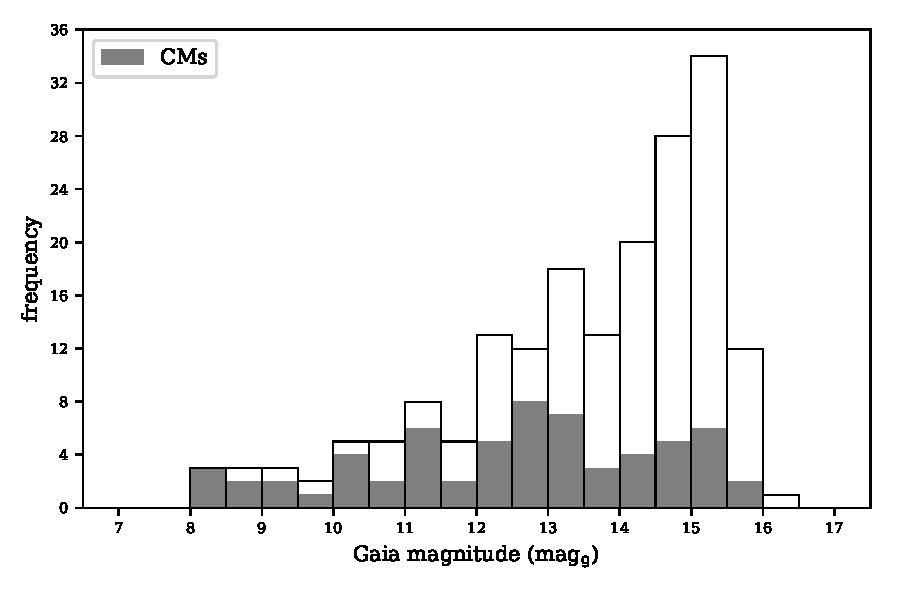
\includegraphics[trim={0 0.4cm 0 0.2cm},clip,width=0.65\textwidth]{Cluster/M34_histogram_mags.pdf}
  \caption{The distribution of \textit{Gaia}magnitudes of the analyzed stars.}
  \label{fig:M34_histogram_mags}
\end{figure}

\begin{figure}[H]
  \centering
    \includegraphics[trim={0 0.5cm 0 0.5cm},clip,width=0.97\textwidth]{Cluster/M34_pm_scatter_sigma.pdf}
  \caption{The proper motions of all analyzed stars including the proper motion of the cluster (red) extracted in figure \ref{fig:M34_histogram_all}. The right side is a zoom-in of the left side.}
  \label{fig:M34_pm_scatter_sigma}
\end{figure}

\begin{figure}[H]
  \centering
    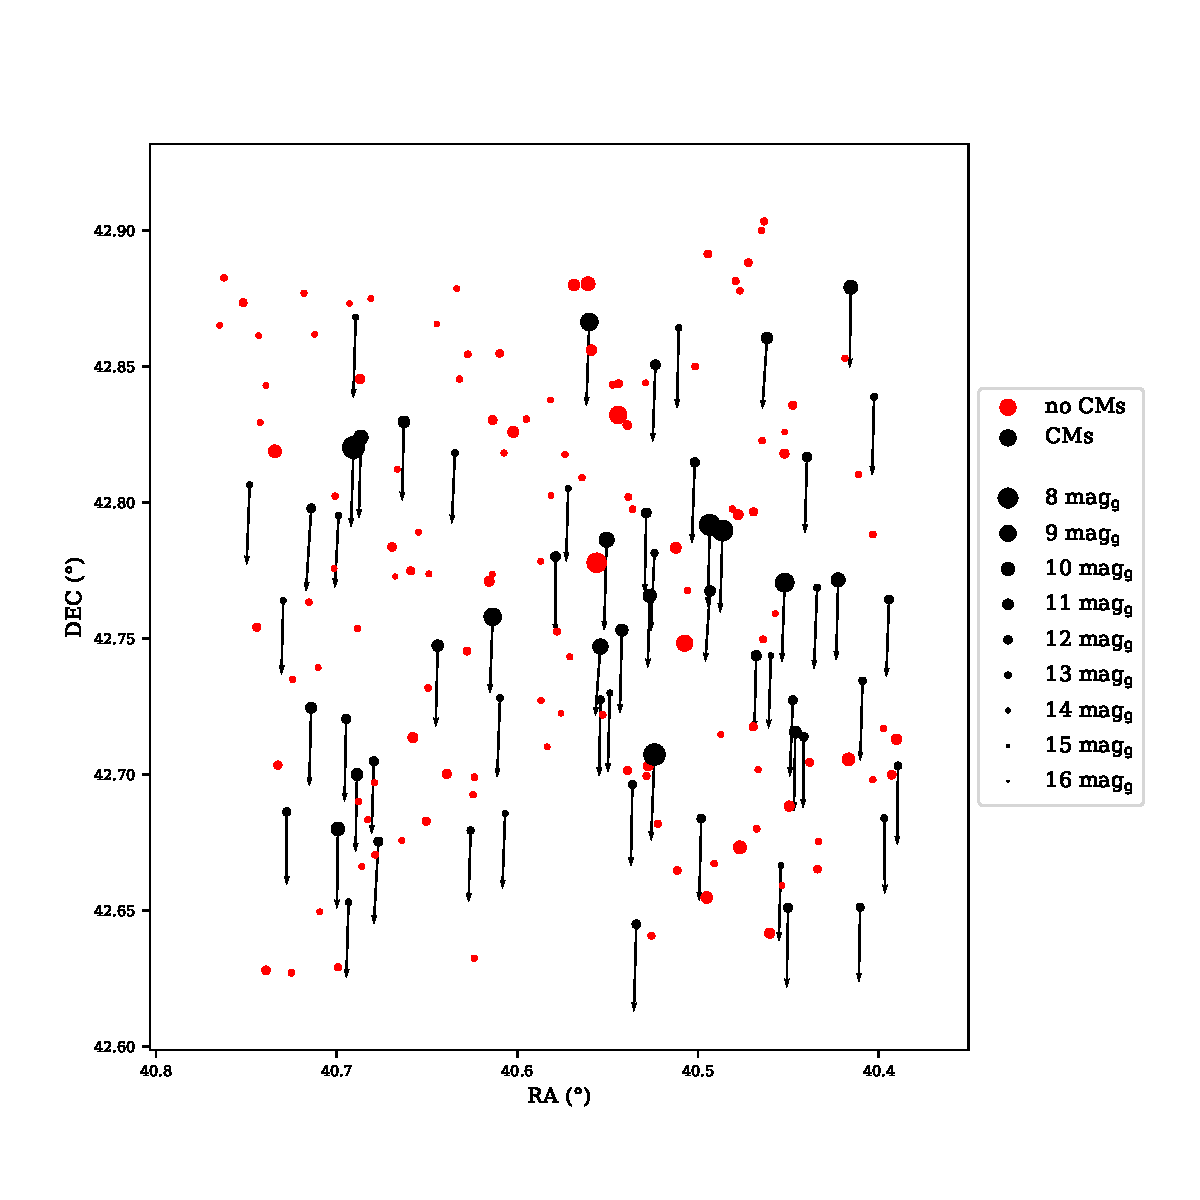
\includegraphics[trim={0 1.6cm 0 2.3cm},clip,width=0.95\textwidth]{Cluster/M34_pm_mask.pdf}
  \caption{Similar to figure \ref{fig:M34_pm} yet just including our cluster members (CMs).}
  \label{fig:M34_pm_mask}
\end{figure}

Those last few plots clearly show us that those stars really make up a cluster. Our cluster distance of (509 $\pm$ 26) pc agrees with the literature value of 513 pc \cite{Cantat2018}. We want to bring up that SIMBAD incorrectly classifies some stars as member stars of M34. E.g. \textit{Gaia DR2 337177889338182400\footnote{\url{http://simbad.u-strasbg.fr/simbad/sim-basic?Ident=Gaia+DR2+337177889338182400&submit=SIMBAD+search}}} - this star has a distance of (126 $\pm$ 1) pc according to \textit{Gaia}. This would be about 400 parsec away from the core of the cluster. 

\paragraph{Teutsch 55}

\begin{figure}[H]
  \centering
    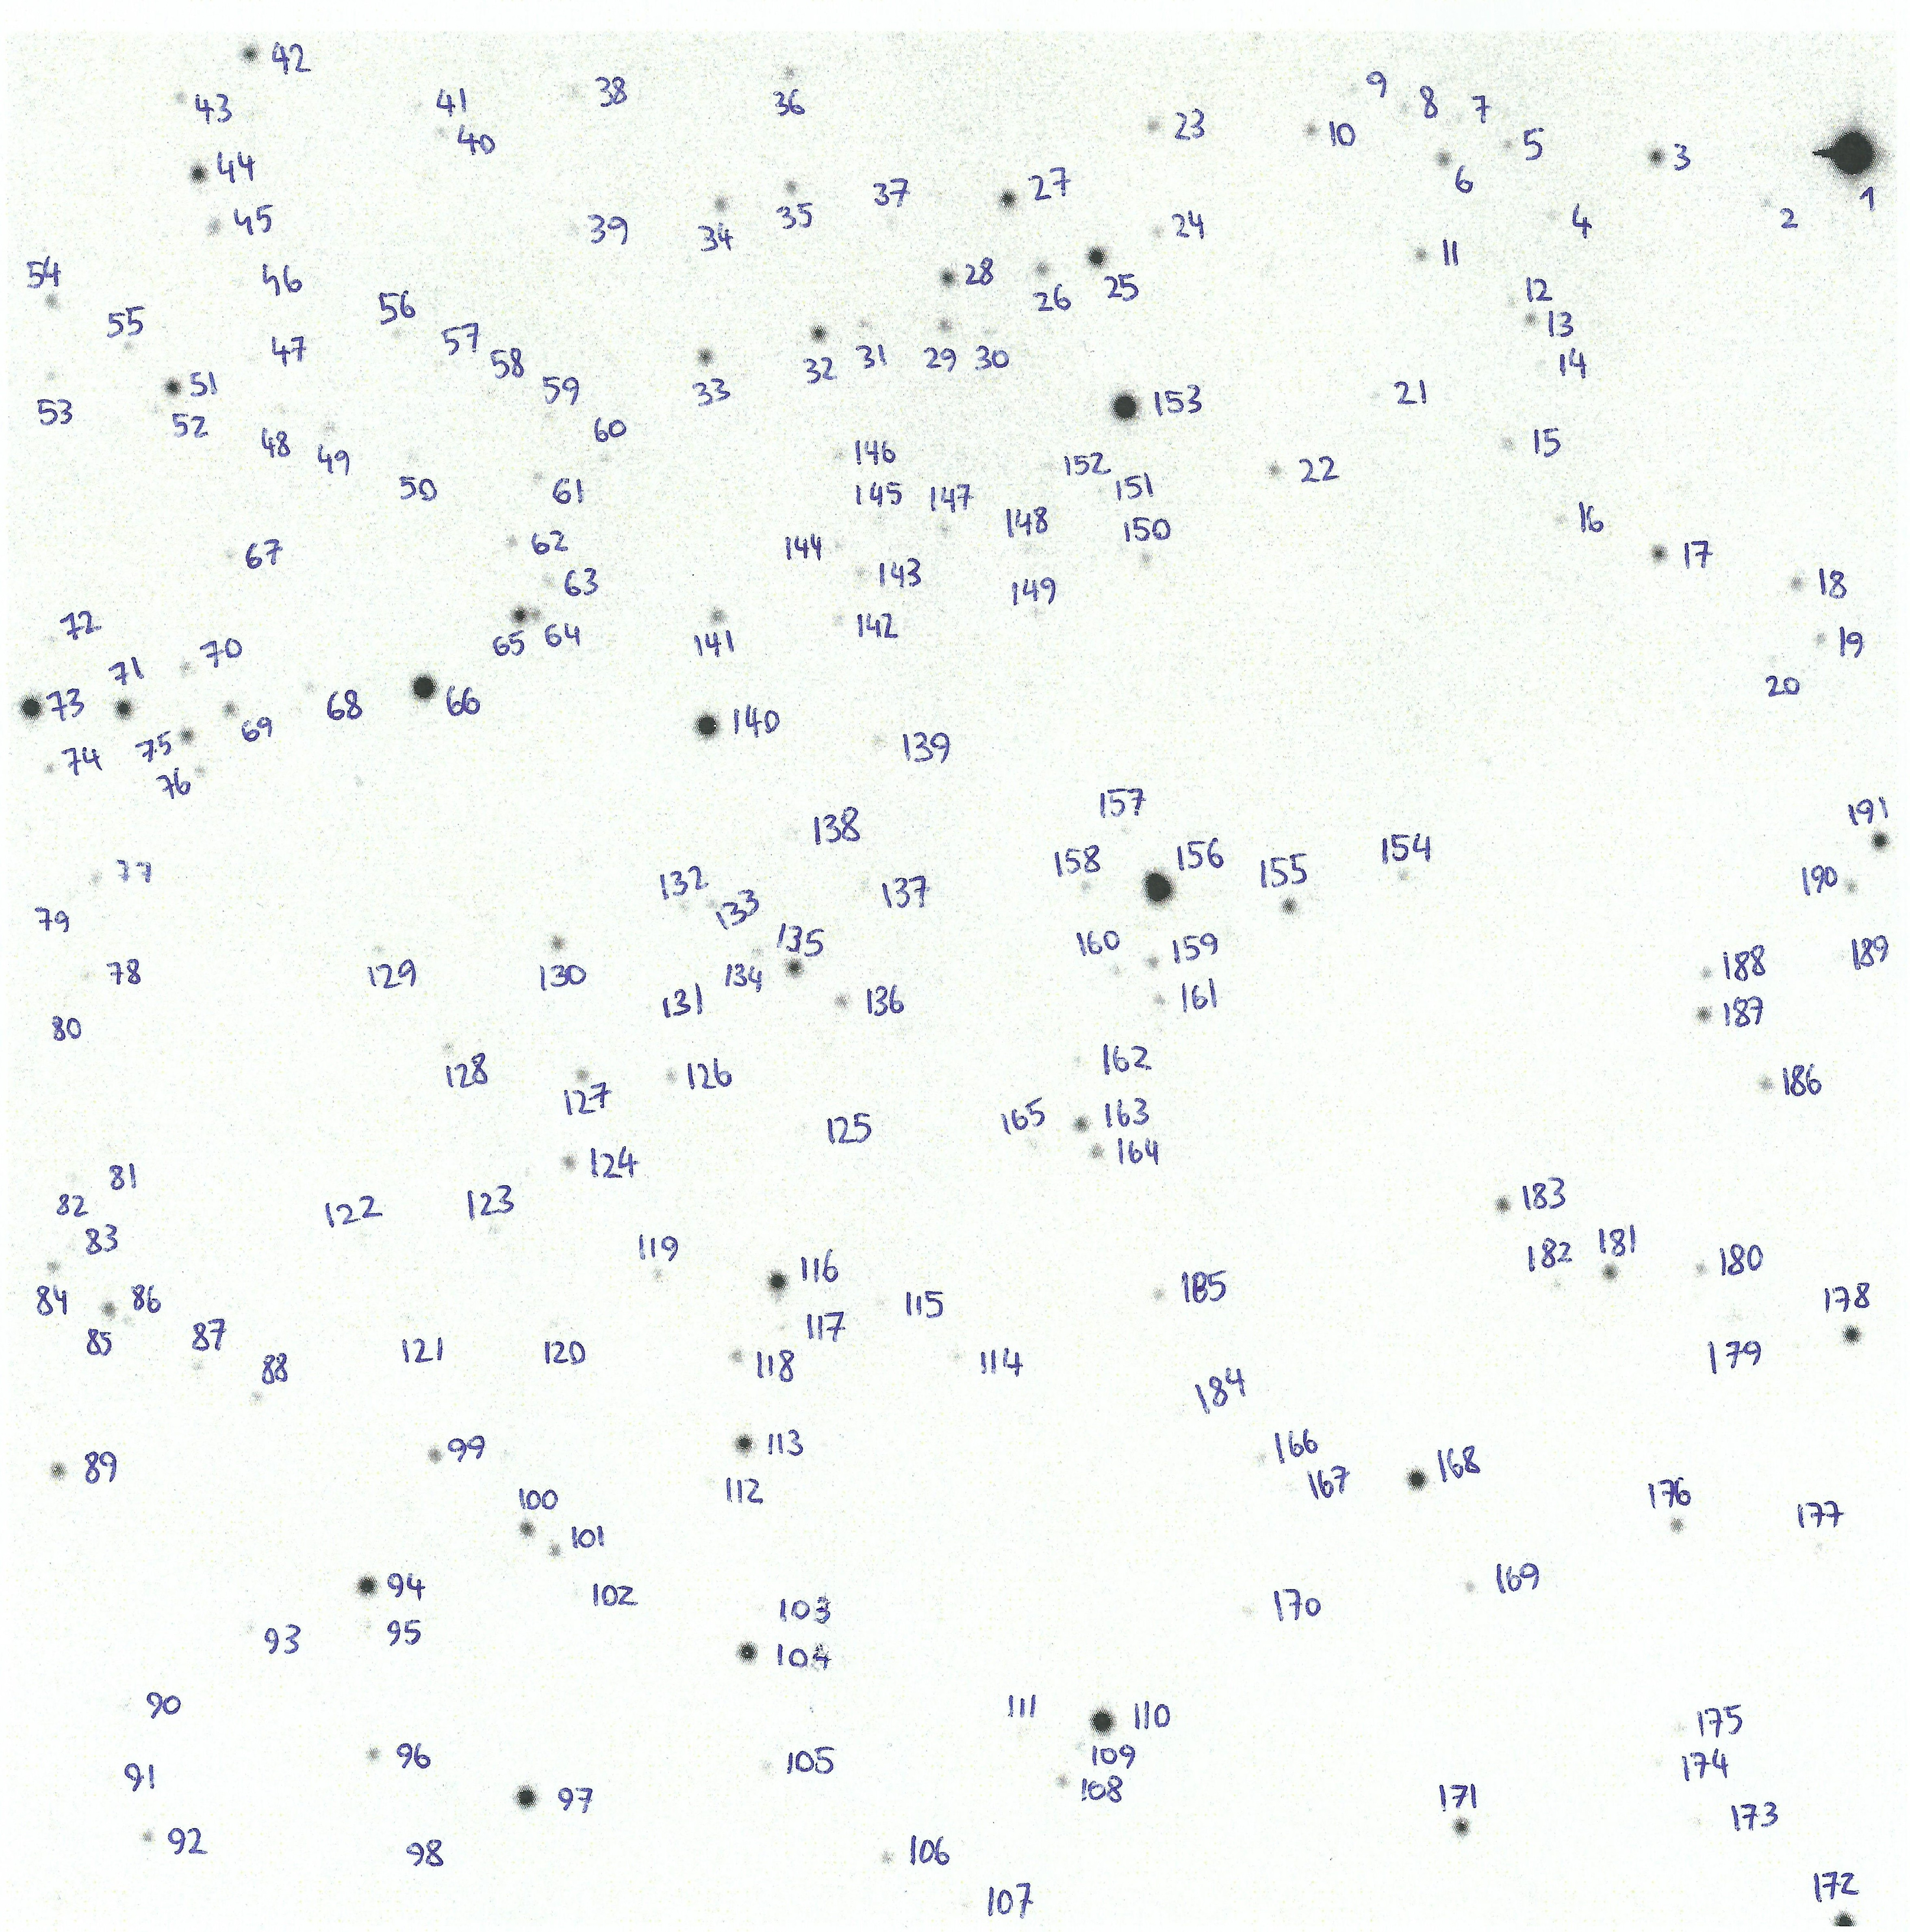
\includegraphics[width=0.95\textwidth]{Cluster/obsTeutsch55_num.jpg}
  \caption{Our observation of Teutsch 55 in the red filter with an exposure time of 300 seconds. The numbers are in correspondence with those in image \ref{fig:DSS2Teutsch55_num}.}
  \label{fig:obsTeutsch55_num}
\end{figure}

\begin{figure}[H]
  \centering
    \includegraphics[width=0.95\textwidth]{Cluster/DSS2Teutsch55_num.jpg}
  \caption{The negative of the observation of Teutsch 55 by the DSS2. This picture was extracted from \textit{Aladin}. The numbers are in correspondence with those in image \ref{fig:obsTeutsch55_num}.}
  \label{fig:DSS2Teutsch55_num}
\end{figure}

\begin{figure}[H]
  \centering
    \includegraphics[trim={0 1.6cm 0 2.3cm},clip, width=0.95\textwidth]{Cluster/Teutsch55_pm.pdf}
  \caption{Every point is an extracted source. The size corresponds to the \textit{Gaia}magnitude. The arrows illustrate the direction of the proper motion. A star was for example not analyzed if the proper motions were missing.}
  \label{fig:Teutsch55_pm}
\end{figure}


\begin{figure}[H]
  \centering
    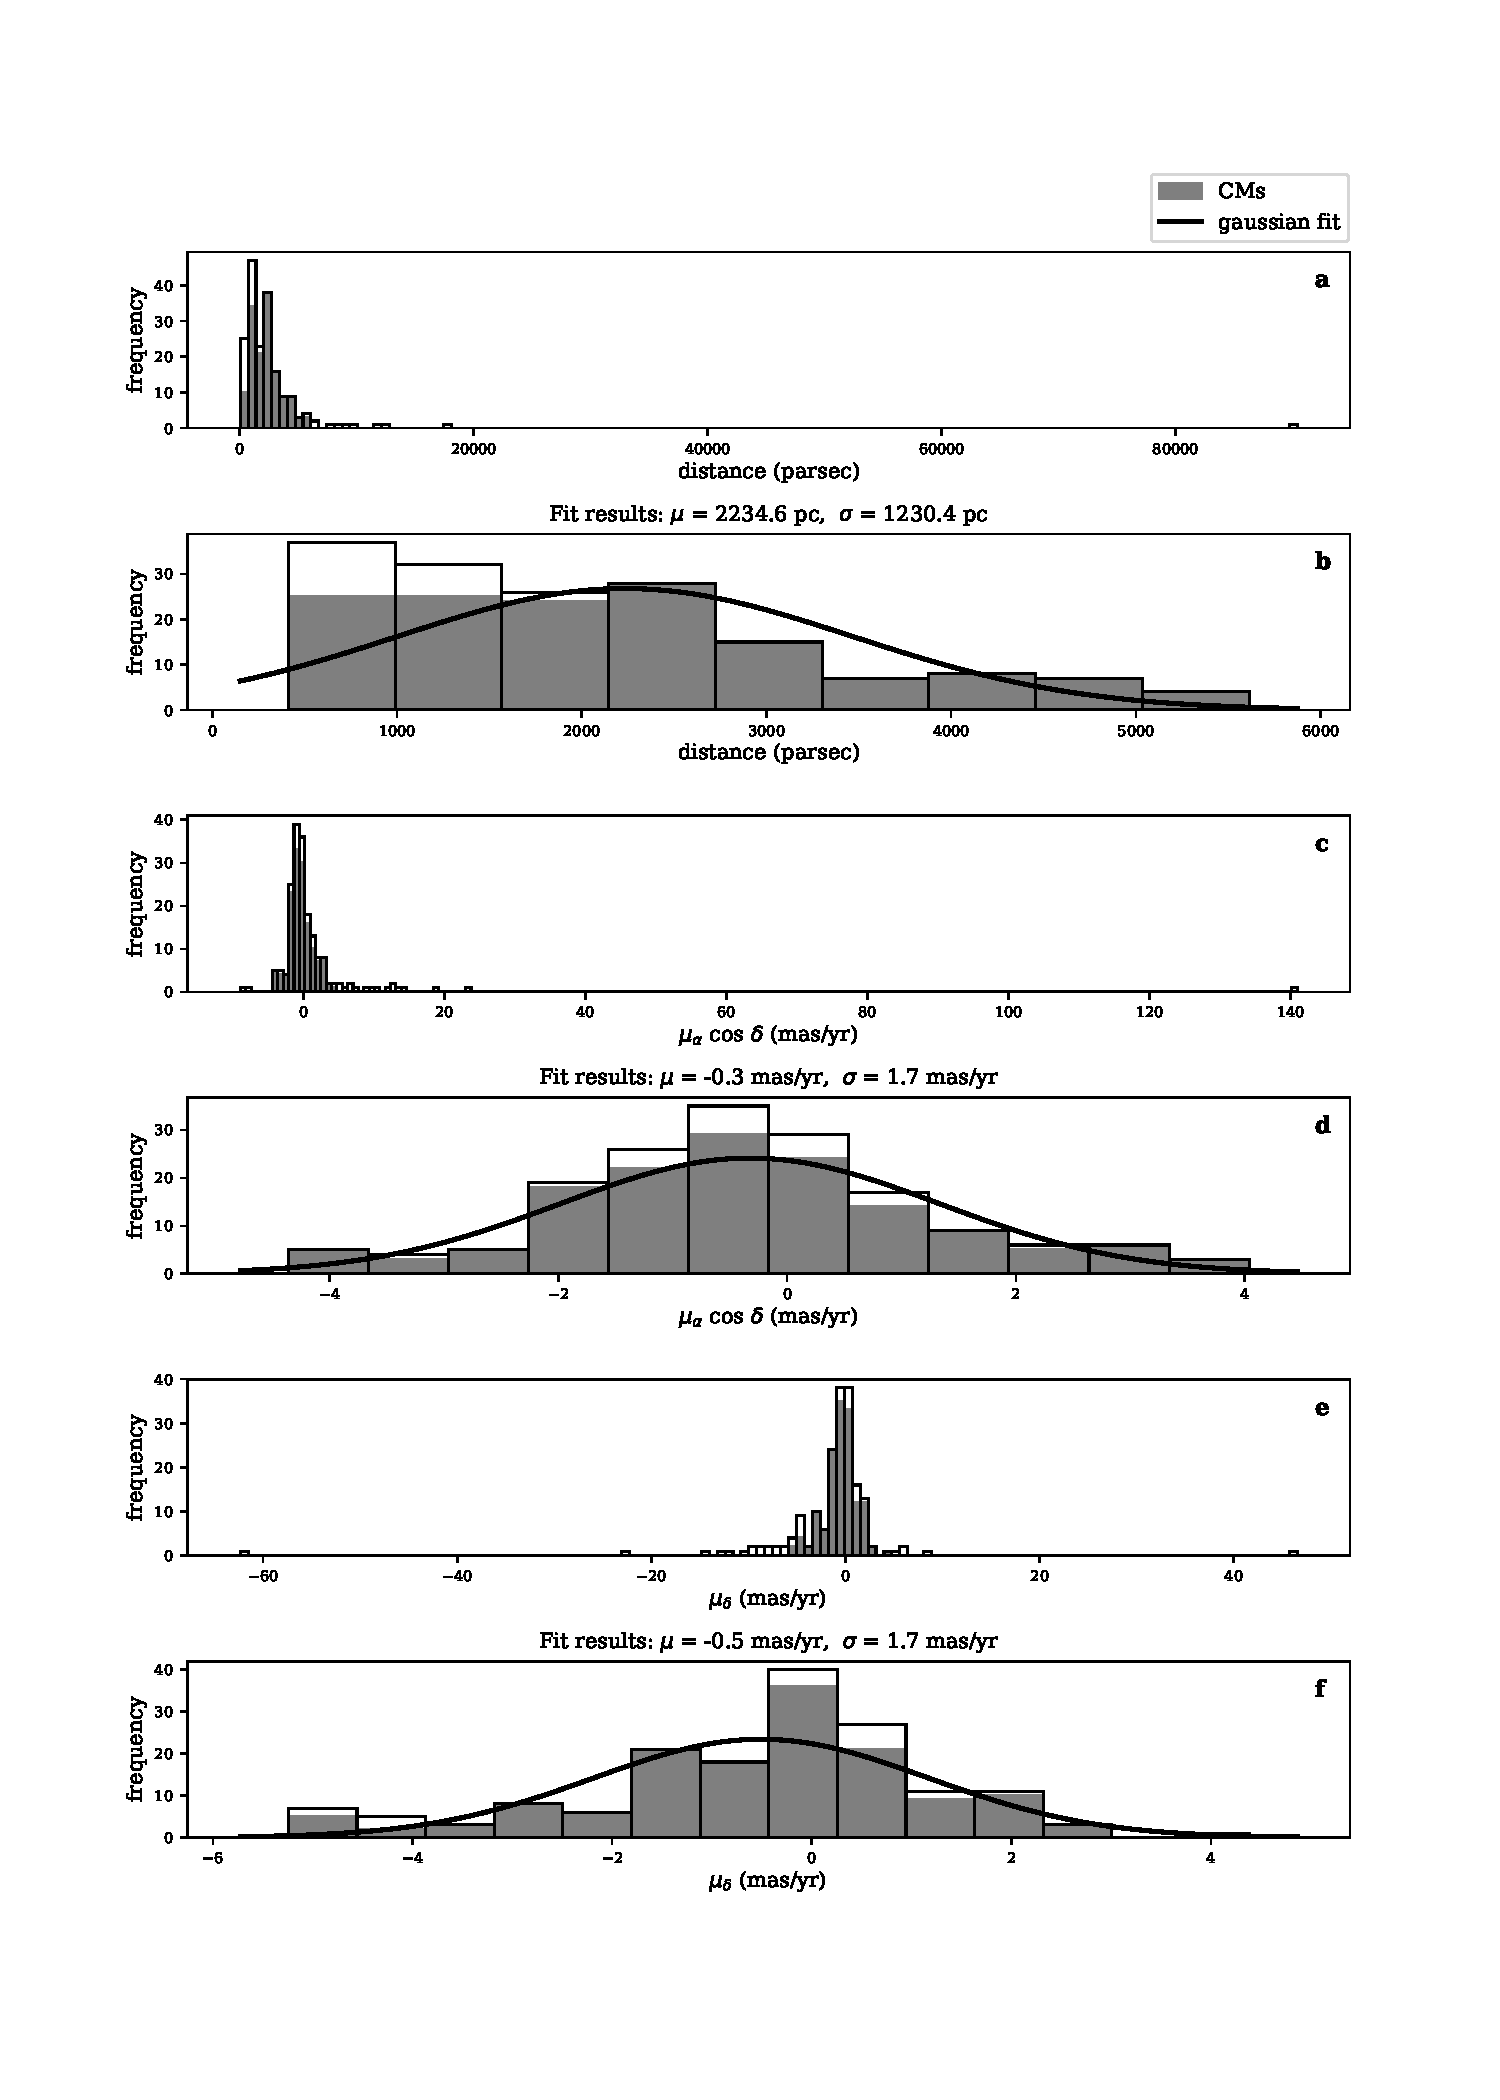
\includegraphics[trim={0 3.4cm 0 2.9cm},clip,width=0.95\textwidth]{Cluster/Teutsch55_histogram_all.pdf}
  \caption{Histogram of the analysed stars. In order to determine the Cluster members (CMs) an iterative sigma clipping procedure was applied (see point 8 in section \ref{sec:Gaia}). \textbf{a, c, e}: The distances and proper motions for all stars and the CMs (in gray). \textbf{b, d, f}: This zoom-in also includes a gaussian fit of the CMs. Above those plots the mean and standard deviation of this gaussian.}
  \label{fig:Teutsch55_histogram_all}
\end{figure}

\begin{figure}[H]
  \centering
    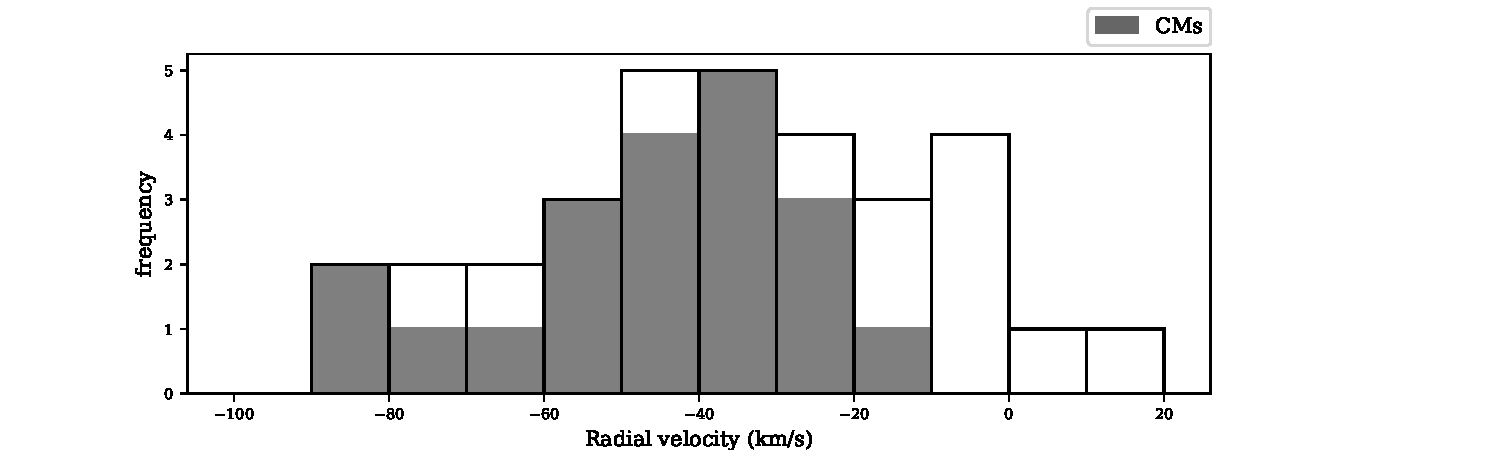
\includegraphics[trim={0 0 2cm 0},clip,width=0.95\textwidth]{Cluster/Teutsch55_histogram_RV.pdf}
  \caption{A histogram of the radial velocities. In gray our cluster members determined with figure \ref{fig:Teutsch55_histogram_all}. We see that non of the outliers are also CMs. This is what we would expect.}
  \label{fig:Teutsch55_histogram_RV}
\end{figure}

\begin{figure}[H]
  \centering
    \includegraphics[trim={0 0.4cm 0 0.2cm},clip,width=0.65\textwidth]{Cluster/Teutsch55_histogram_mags.pdf}
  \caption{The distribution of \textit{Gaia}magnitudes of the analyzed stars.}
  \label{fig:Teutsch55_histogram_mags}
\end{figure}

\begin{figure}[H]
  \centering
    \includegraphics[trim={0 0.5cm 0 0.5cm},clip,width=0.97\textwidth]{Cluster/Teutsch55_pm_scatter_sigma.pdf}
  \caption{The proper motions of all analyzed stars including the proper motion of the cluster (red) extracted in figure \ref{fig:Teutsch55_histogram_all}. The right side is a zoom-in of the left side.}
  \label{fig:Teutsch55_pm_scatter_sigma}
\end{figure}

\begin{figure}[H]
  \centering
    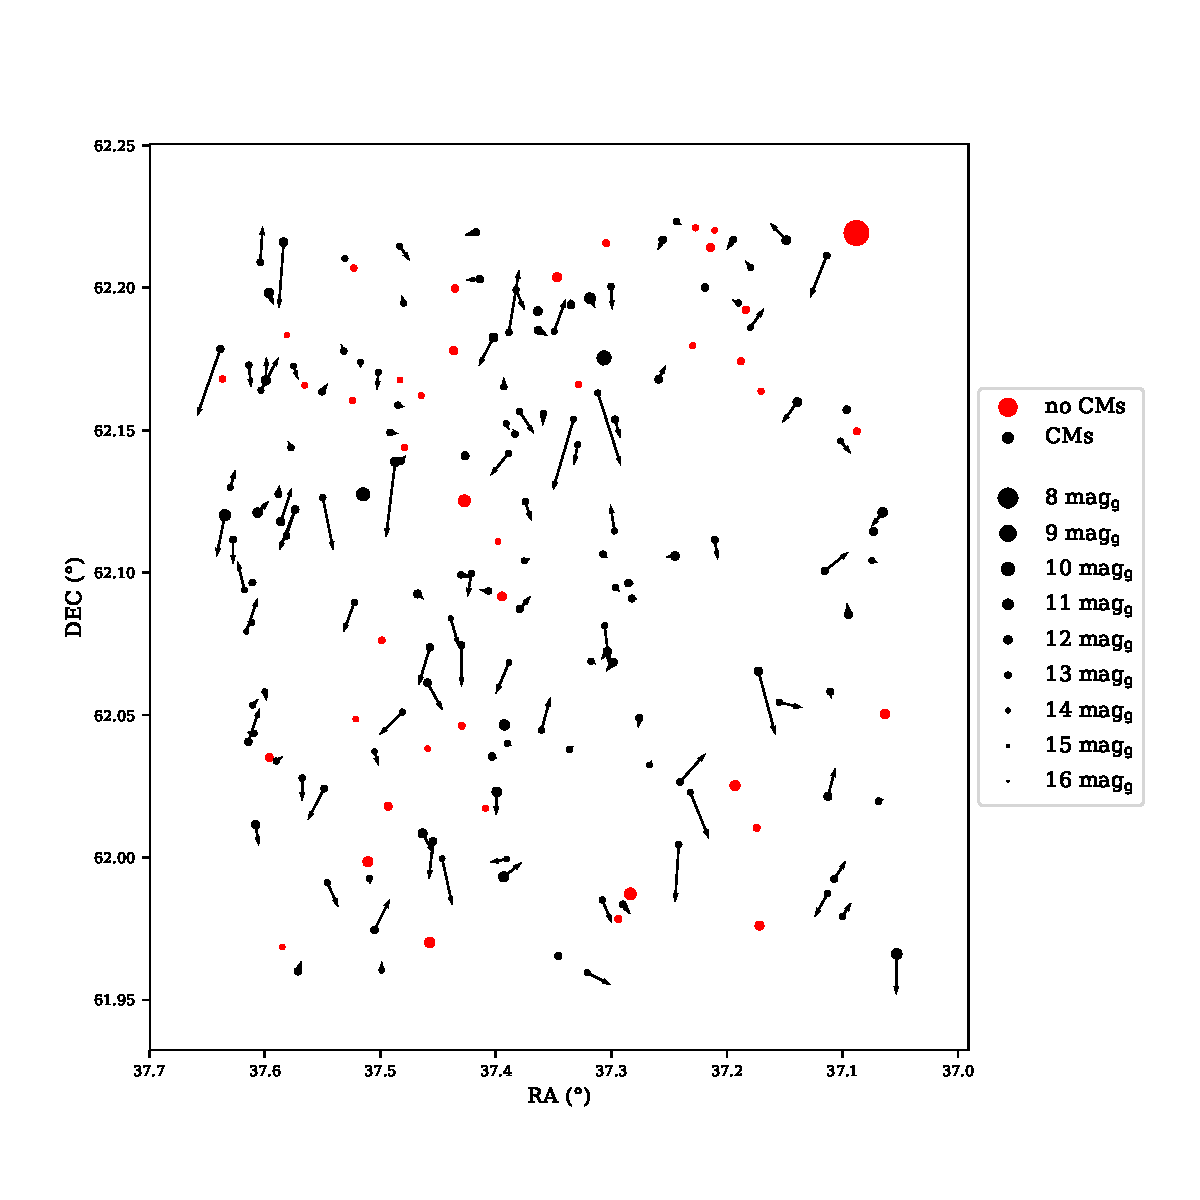
\includegraphics[trim={0 1.6cm 0 2.3cm},clip,width=0.95\textwidth]{Cluster/Teutsch55_pm_mask.pdf}
  \caption{Similar to figure \ref{fig:Teutsch55_pm}, however just including our cluster members (CMs).}
  \label{fig:Teutsch55_pm_mask}
\end{figure}

In contrast M34 (cf.~\ref{fig:M34_pm_mask}) we do not see, that those stars are moving as a group in one direction. We also see this very broad distribution in distances and proper motions in figure \ref{fig:Teutsch55_histogram_all}. So we cannot really confirm this cluster.

\paragraph{Stock 19 (C0001+557)}

\begin{figure}[H]
  \centering
    \includegraphics[width=0.95\textwidth]{Cluster/obsStock19_num.jpg}
  \caption{Our observation of Stock 19 in the red filter with an exposure time of 200 seconds. The numbers are in correspondence with those in image \ref{fig:DSS2Stock19_num}.}
  \label{fig:obsStock19_num}
\end{figure}

\begin{figure}[H]
  \centering
    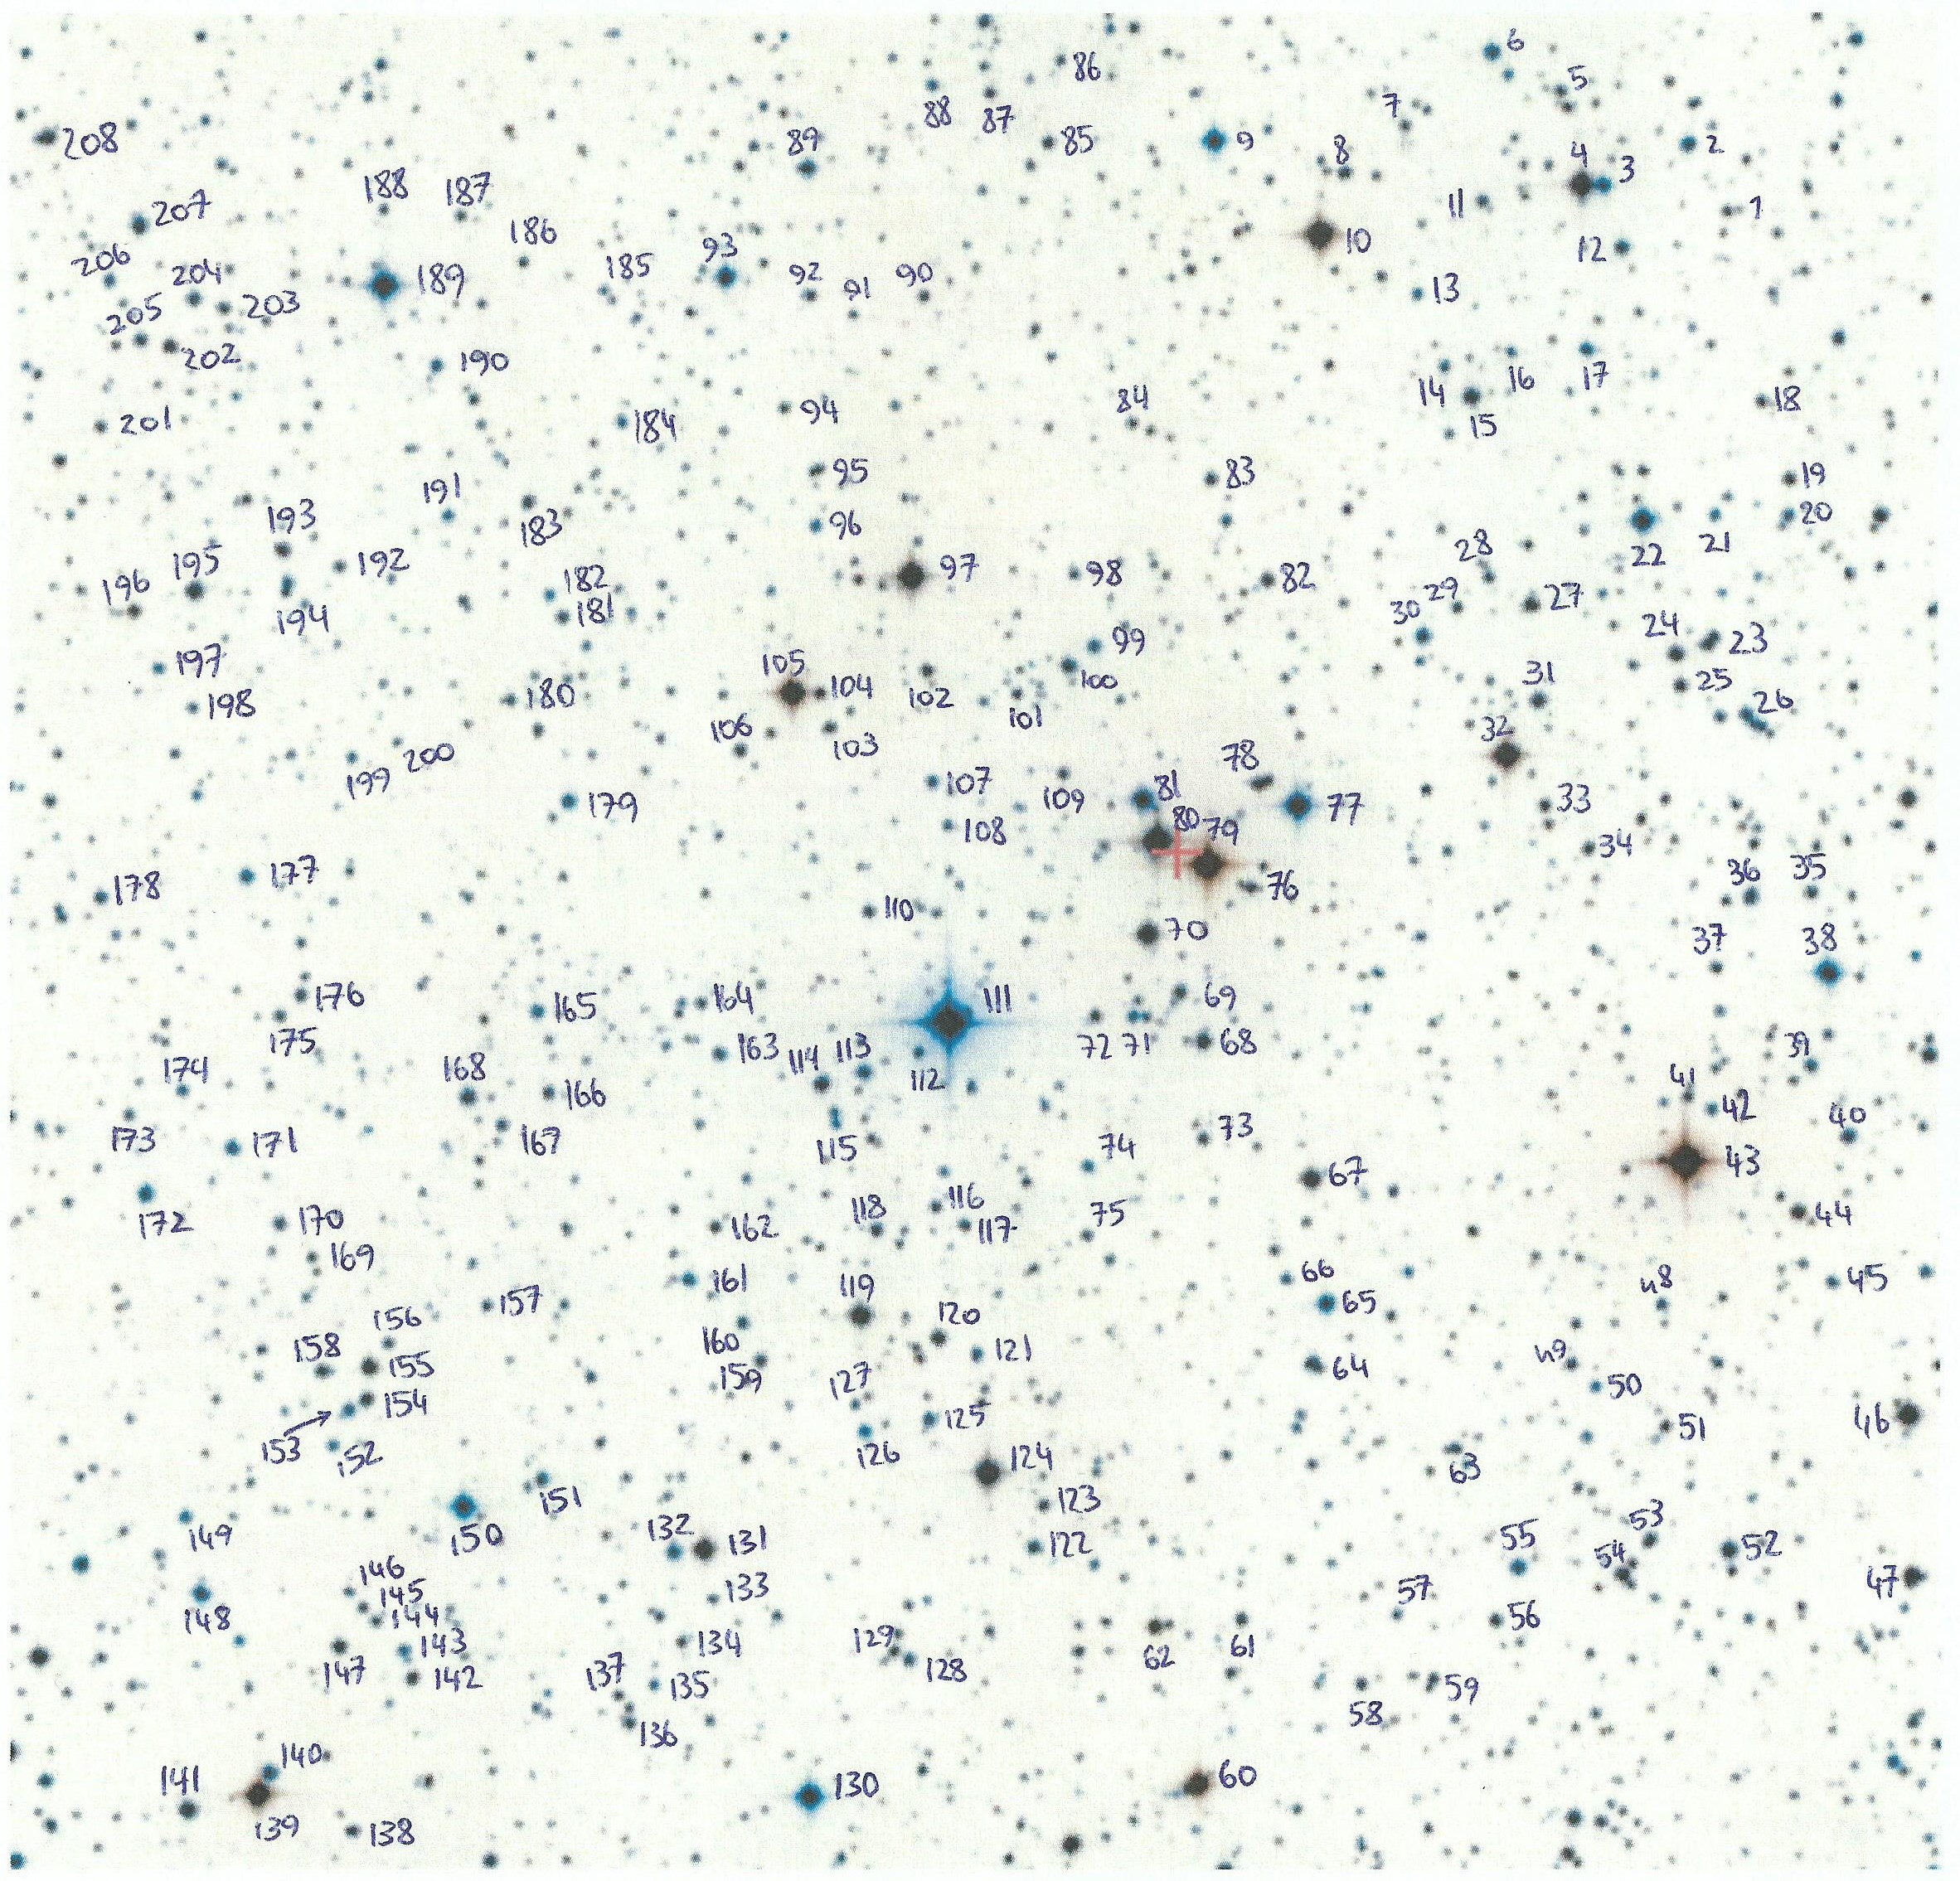
\includegraphics[width=0.95\textwidth]{Cluster/DSS2Stock19_num.jpg}
  \caption{The negative of the observation of Stock 19 by the DSS2. This picture was extracted from \textit{Aladin}. The numbers are in correspondence with those in image \ref{fig:obsStock19_num}.}
  \label{fig:DSS2Stock19_num}
\end{figure}

The only light source we observed - of the about 600 in total - without a \textit{Gaia DR2} entry is star 124 (in the lower middle of \ref{fig:obsStock19_num} and \ref{fig:DSS2Stock19_num}) known as TYC 3656-465-1. The specific reason that this star has no \textit{Gaia}entry is unknown. It however has a 2MASS entry. The stars magnitude is at about 11 (visual).  

\begin{figure}[H]
  \centering
    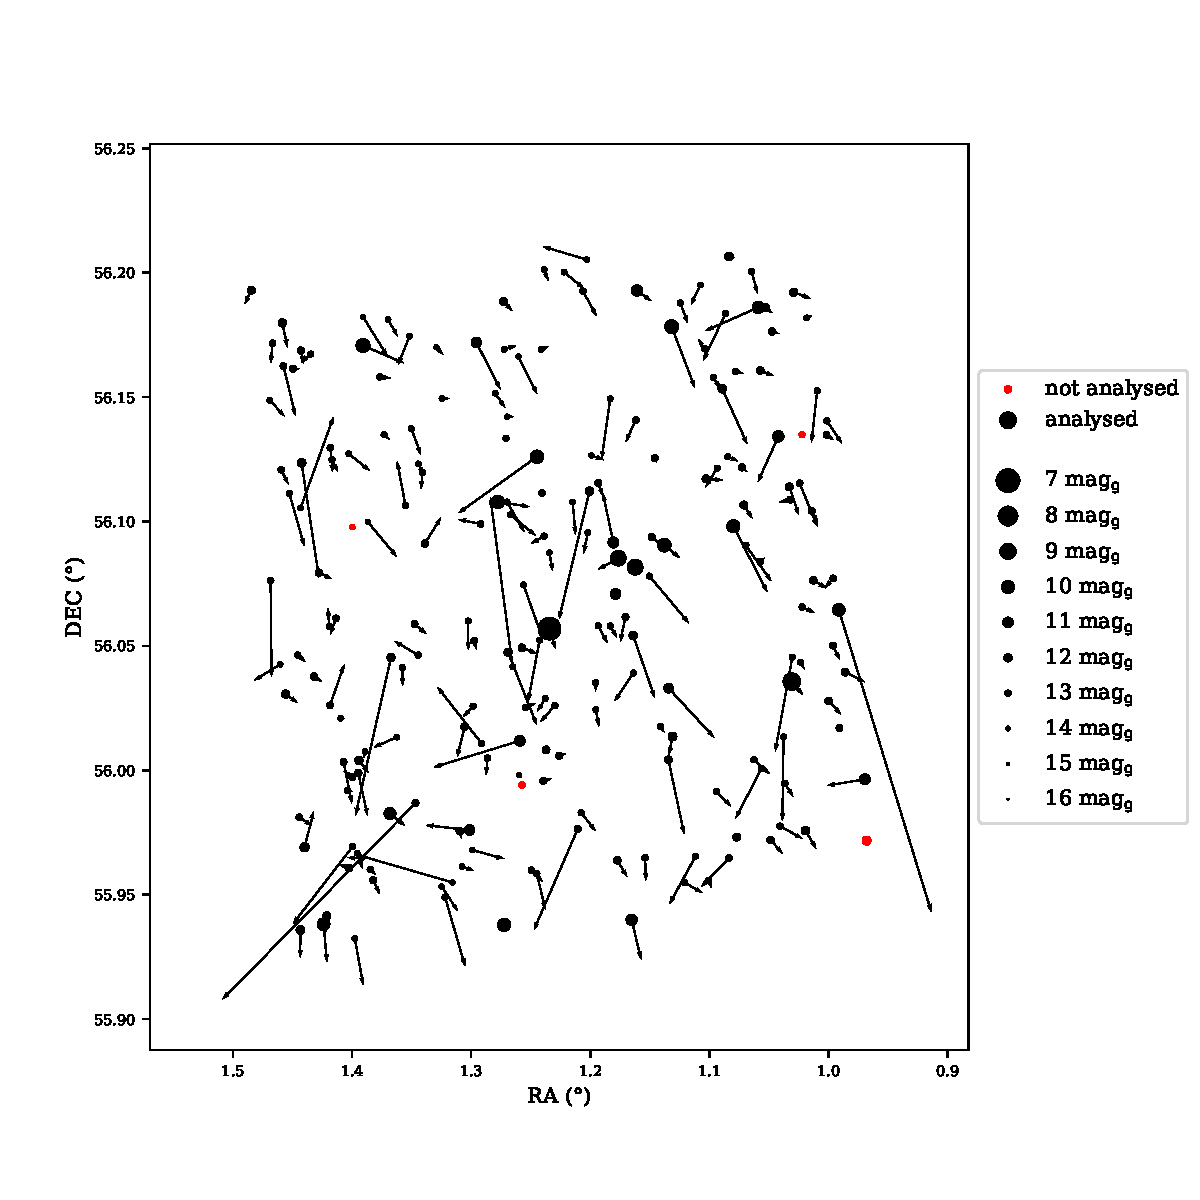
\includegraphics[trim={0 1.6cm 0 2.3cm},clip, width=0.95\textwidth]{Cluster/Stock19_pm.pdf}
  \caption{Every point is an extracted source. The size corresponds to the \textit{Gaia}magnitude. The arrows illustrate the direction of the proper motion. A star was for example not analyzed if the proper motions were missing.}
  \label{fig:Stock19_pm}
\end{figure}

\begin{figure}[H]
  \centering
    \includegraphics[trim={0 3.4cm 0 2.9cm},clip,width=0.95\textwidth]{Cluster/Stock19_histogram_all.pdf}
  \caption{Histogram of the analysed stars. In order to determine the Cluster members (CMs) an iterative sigma clipping procedure was applied (see point 8 in section \ref{sec:Gaia}). \textbf{a, c, e}: The distances and proper motions for all stars and the CMs (in gray). \textbf{b, d, f}: This zoom-in also includes a gaussian fit of the CMs. Above those plots the mean and standard deviation of this gaussian.}
  \label{fig:Stock19_histogram_all}
\end{figure}

\begin{figure}[H]
  \centering
    \includegraphics[trim={0 0 2cm 0},clip,width=0.95\textwidth]{Cluster/Stock19_histogram_RV.pdf}
  \caption{A histogram of the radial velocities. In gray our cluster members determined with figure \ref{fig:Stock19_histogram_all}.}
  \label{fig:Stock19_histogram_RV}
\end{figure}

\begin{figure}[H]
  \centering
    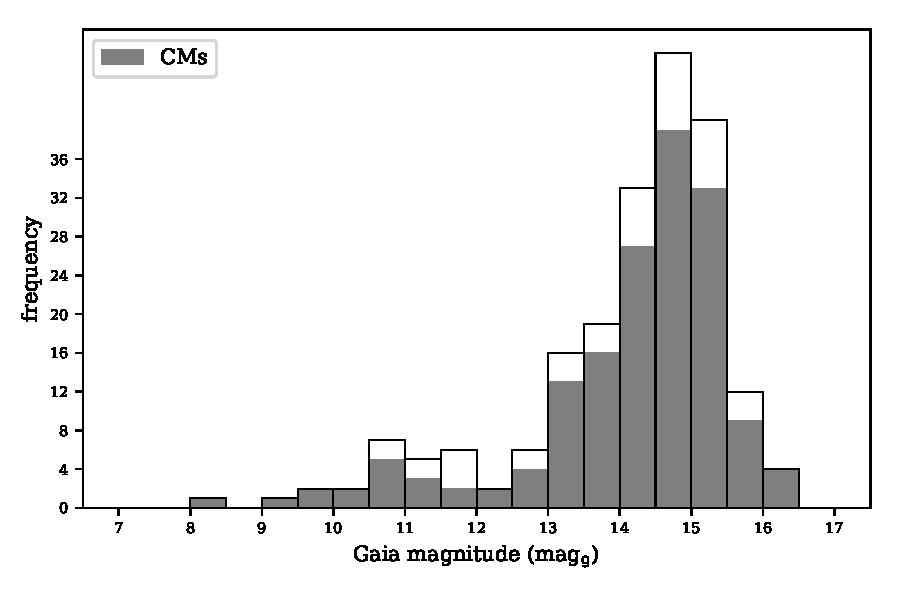
\includegraphics[trim={0 0.4cm 0 0.2cm},clip,width=0.65\textwidth]{Cluster/Stock19_histogram_mags.pdf}
  \caption{The distribution of \textit{Gaia}magnitudes of the analyzed stars.}
  \label{fig:Stock19_histogram_mags}
\end{figure}

\begin{figure}[H]
  \centering
    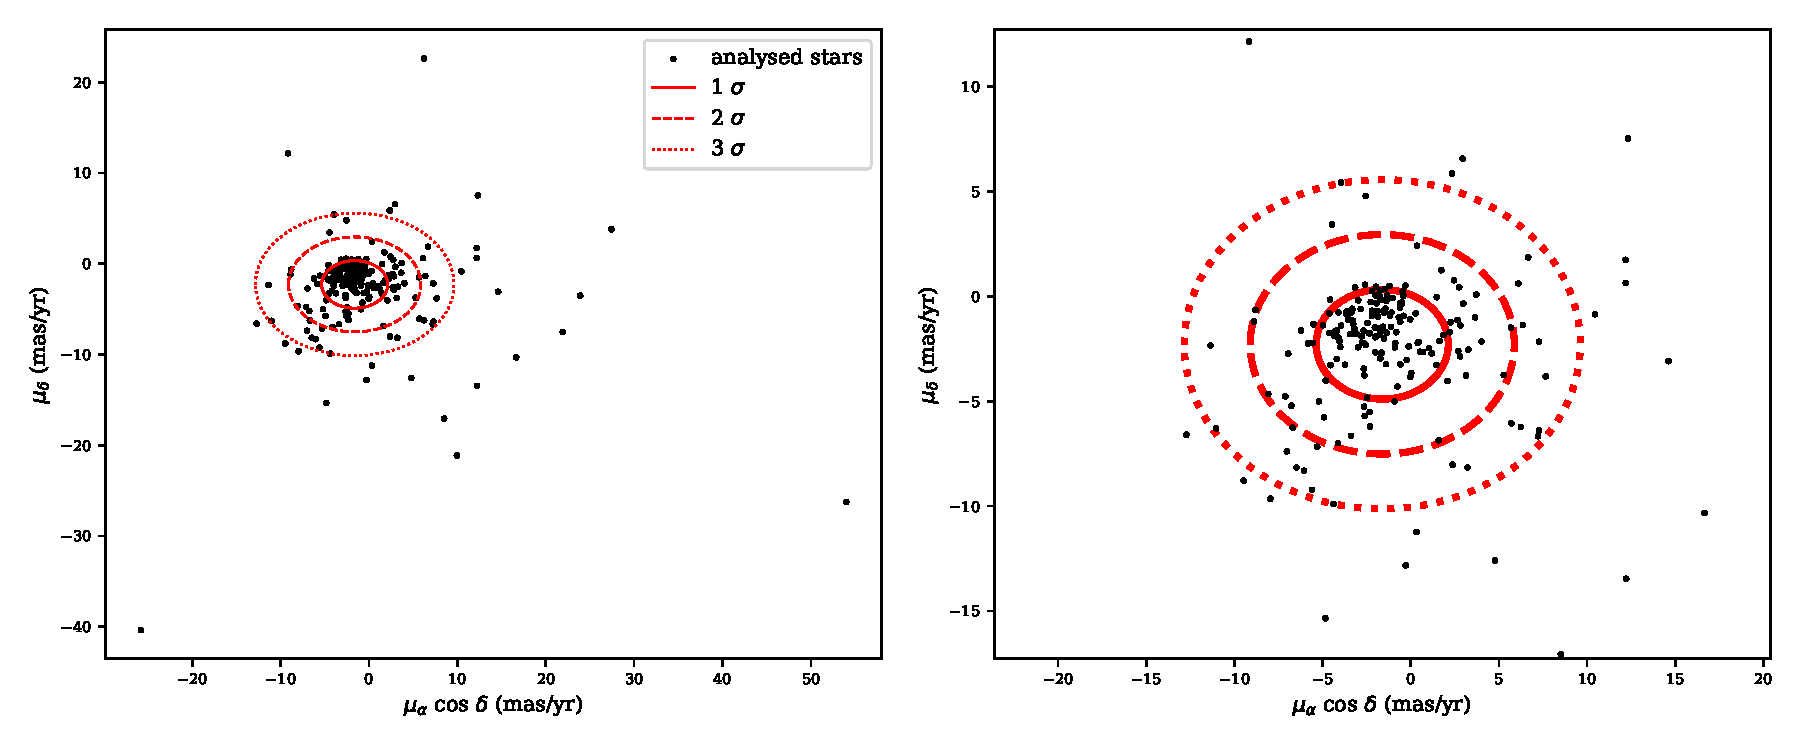
\includegraphics[trim={0 0.5cm 0 0.5cm},clip,width=0.97\textwidth]{Cluster/Stock19_pm_scatter_sigma.pdf}
  \caption{The proper motions of all analyzed stars including the proper motion of the cluster (red) extracted in figure \ref{fig:Stock19_histogram_all}. The right side is a zoom-in of the left side.}
  \label{fig:Stock19_pm_scatter_sigma}
\end{figure}

\begin{figure}[H]
  \centering
    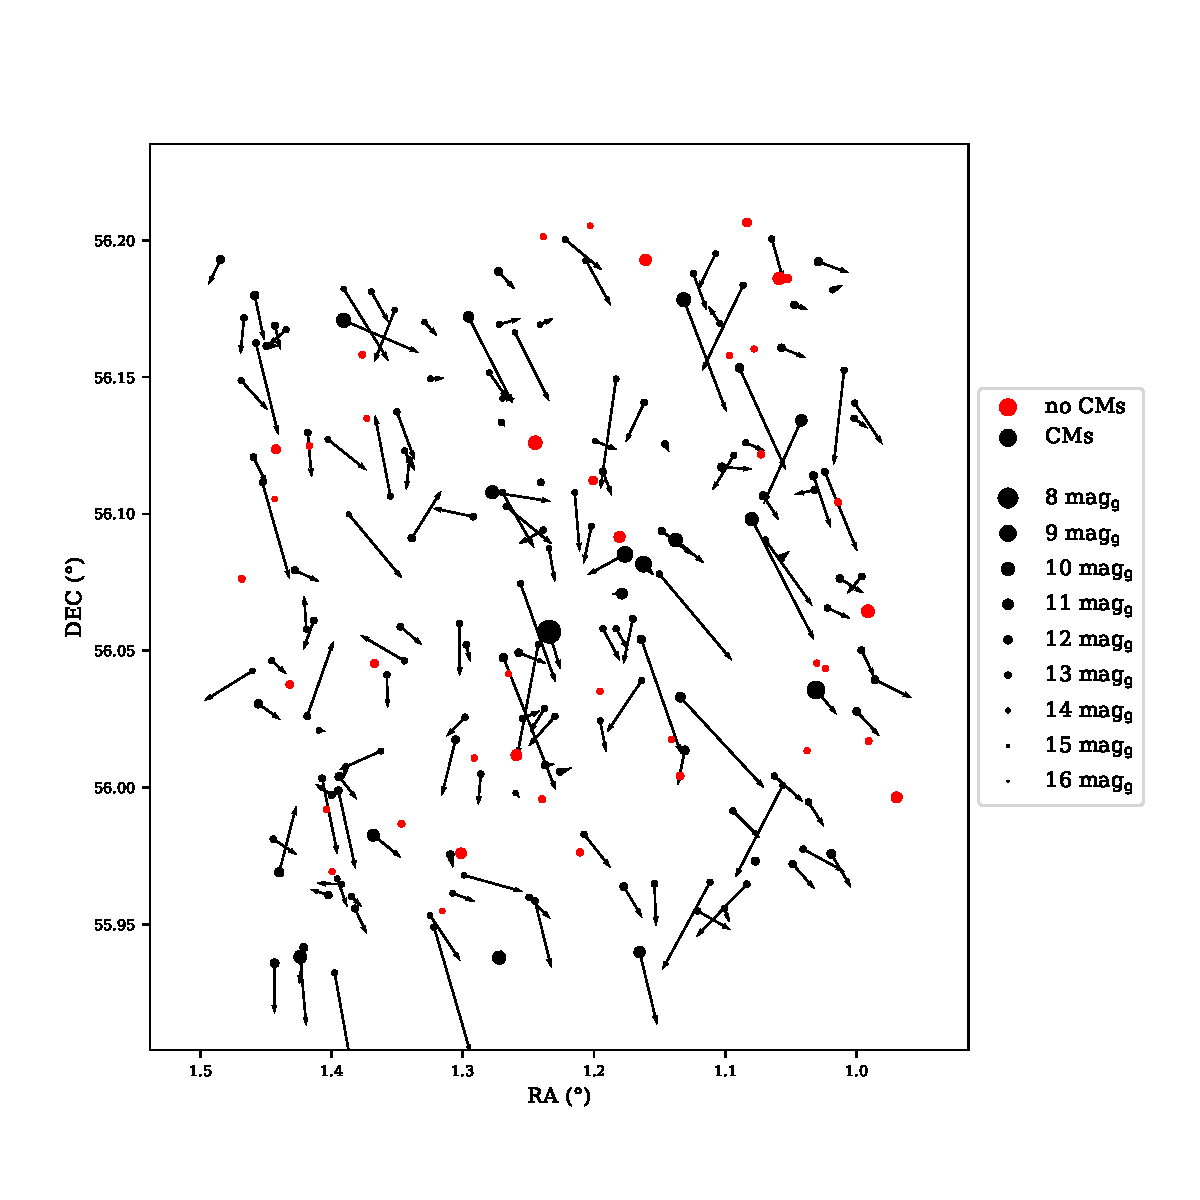
\includegraphics[trim={0 1.6cm 0 2.3cm},clip,width=0.95\textwidth]{Cluster/Stock19_pm_mask.pdf}
  \caption{Similar to figure \ref{fig:Stock19_pm} yet just including our cluster members (CMs).}
  \label{fig:Stock19_pm_mask}
\end{figure}

Similar to figure~\ref{fig:Teutsch55_pm_mask}, but in contrast to figure \ref{fig:M34_pm_mask} we do not see, that those stars are moving as a group in one direction. We also see this very broad distribution in distances and proper motions in figure \ref{fig:Stock19_histogram_all}. So we cannot really confirm this cluster.

To conclude, it proves to be rather difficult to tell whether the imaged objects actually can be classified as galactic open clusters. It might be interesting to look at the color of the suspected cluster members, but we do not have color information for a sufficient amount of stars in the images as extracting sources from the images is not trivial, especially in the Johnson B filter. Furthermore, \textit{Gaia}data has to be studied very thoroughly as often times measured properties are wrong in a very obvious way, for example negative parallaxes can be found for several stars.  

\subsection{Imaging using a lucky imager}

Lucky imaging is a technique used to counteract the negative influence of the turbulence in the air of the Earth's atmosphere. During long exposures the movement of the atmosphere smears out the imaged object which results in sub optimal images. Therefore the idea is to reduce exposure time to a minimum by basically taking a video of the object one wants to image. From the video one can select the frame or frames which show the least amount of turbulence in the atmosphere. This technique is therefore only nicely applicable for setups and sources which do not require long exposure times.

In practice the selection of high quality frames is not done manually but with an automated software algorithm like the one used by Autostakkert~\parencite{autostakkert}, which we use for generating the images taken with the lucky imaging camera. Software like this automatically stacks single frames from a video which have a high quality according to an algorithm which looks at, for example, the FWHM of stars or the surface structures on the Moon. For stacking, the images are aligned using the brightest pixels as reference before being combined. Afterwards it is possible to apply artificial sharpening via a convolution. 

The influence of this sharpening convolution can be seen in figure~\ref{fig:moon_comp_sharp} and the overall improvement which can be achieved using lucky imaging is shown in figure~\ref{fig:moon_comp_av}. The videos from which these images are generated are taken with the 60cm telescope and the lucky imaging camera on December $13^\text{th}$ while waiting for the comet 46P/Wirtanen to appear above the horizon. As already mentioned in the section about imaging this comet, the seeing was not great that night however the lucky images of the moon are of an impressively high quality given the setup and location. 

\begin{figure}[H]
\centering
\begin{minipage}{1.\textwidth}
\centering
  \includegraphics[width=0.9\textwidth]{Lucky_Imaging/moon1_stack.pdf}
\end{minipage}
\begin{minipage}{1.\textwidth}
\centering
  \includegraphics[width=0.9\textwidth]{Lucky_Imaging/moon1_stack_conv.pdf}
\end{minipage}
    \caption{Comparison of a stacked image generated from the best 27\% of frames of a 1000 frames movie of the Moon (upper image) using the Autostakkert software \parencite{autostakkert} and a sharpened version of the same stacked image (lower image). An automatic convolution is applied to the stacked image in order to obtain the sharpened version.} 
    \label{fig:moon_comp_sharp}
\end{figure}

\begin{figure}[H]
\centering
\begin{minipage}{1.\textwidth}
\centering
  \includegraphics[width=0.865\textwidth]{Lucky_Imaging/moon1_bad.pdf}
\end{minipage}
\begin{minipage}{1.\textwidth}
\centering
  \includegraphics[width=0.865\textwidth]{Lucky_Imaging/moon2_stack_conv.pdf}
\end{minipage}
    \caption{Comparison of an arbitrarily chosen frame of a video of a different part of the Moon (upper image) and the final sharpened version produced from the same video by stacking the top 25\% of frames and sharpening. This was also done using Autostakkert \parencite{autostakkert}. The improvement can easily be seen when comparing both images.}
    \label{fig:moon_comp_av}
\end{figure}

\section{Spectroscopy}\label{sec:spectrum}
In this section of our report, we describe the methods of spectroscopy using the Lhires III spectrograph. Subsection~\ref{ss:1} gives a summary of observational methods including a short overview of the inner workings of a Littrow-Spectrograph and the means of preparation in order to reduce the taken spectra. In subsection~\ref{ss:2} we report on how to reduce and extract a spectrum from a CCD image using IRAF. Continuing in subsection~\ref{ss:3} we show how to map CCD pixel number to a wavelength scale in order to calibrate the spectrum and how to normalize the continuum. Finishing up in~\ref{ss:4} we will discuss observed spectra from two well known sources (Vega - $\alpha$ Lyrae  $\&$ Deneb - $\alpha$ Cygni) concerning problems that our method of observation may show. 
\subsection{Observational methods \& preparation}
\label{ss:1}
As documented in~\parencite{Shelyak_Instruments} Lhires III (\underline{L}ittrow \underline{H}igh \underline{RE}solution \underline{S}pectrograph) is a spectrograph in Littrow configuration meaning it has an optical path and general structure as in figure~\ref{fig:1}. Rendering this special kind of setup for a spectrograph, both compact and affordable, the Littrow configuration is defined by having the same optical element - a 200mm lens - be both the collimator, parallelizing the beam, and the imaging lens at once. The diffraction grating (300 lines per mm) allows for expected spectral dispersions of $\SI{1.493}{\angstrom\per\pixel}$. In the vicinity of the H Alpha line in the red part of the spectrum, the resolving power $\frac{\Delta\lambda}{\lambda}$ is approximately $1300$. A spreadsheet ~\parencite{Shelyak_Instruments} with simulated results, assuming a telescope aperture of $\text{D}=\SI{60}{\cm}$ and a focal ratio $\frac{\text{F}}{\text{D}}=8$, defines the limiting magnitude in a one hour ($\frac{\text{S}}{\text{N}}=\num{100}$) exposure to be $\text{m}=\num{11.3}$, when simulated with a target star of type B0V.\\
\begin{figure}[H]
	\centering
	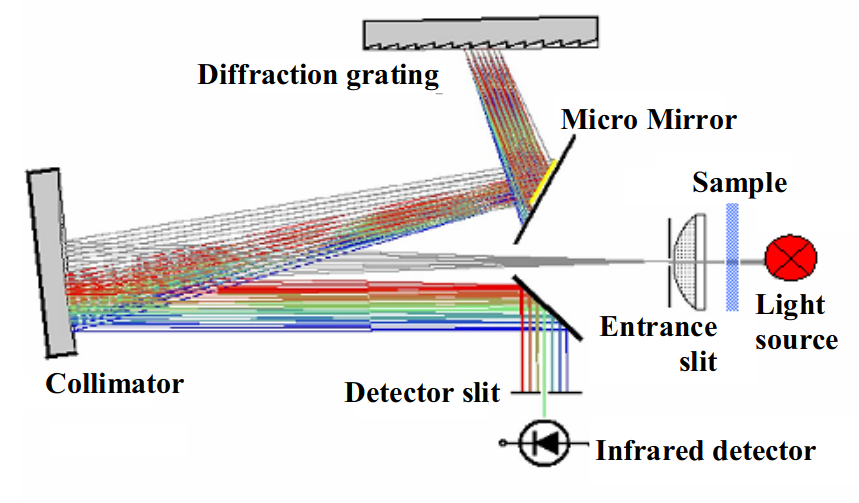
\includegraphics[width=0.75\textwidth]{spectroscopy/littrow.png}
	\caption{Here one can see the general structure and optical path of a spectrograph in Littrow configuration, which is the configuration of Lhires. Image taken from~\parencite{Annual_Report_TU_Chemnitz}}
	\label{fig:1}
\end{figure}

Let us now look at preparation steps to take in order to observe real spectra with this tool. First, since the observation of spectra in this fashion uses CCD imaging, we need to take several bias, dark and flat images to later reduce the images as described in section \ref{ss:2}. Furthermore, calibration images of a neon reference lamp have to be taken in order to do the wavelength calibration~(subsection \ref{ss:3}). One such image of the emission lines of neon and other residual elements can be seen in figure~\ref{fig:2}. The tricky part in taking this image is exposing long enough to have good signal to noise values in the weak emission lines (rightmost part of the image), while not over exposing the strong lines in the center. An exposure time of $t=\SI{10}{\second}$ proved favorable in our case. Once done with taking several of these line calibration images one can start to search for an object on the sky to observe and center it in the middle of the field of view using an imaging camera. Coming to the tricky part of the quest, we now need to focus the image of the object on the entrance slit of the spectrograph. Once this is accomplished an image of the object, such as the spectrum of the star Vega ($\alpha$ Lyrae) with an exposure time of $t=\SI{200}{\second}$, can be taken - see figure \ref{fig:3}. 

\begin{figure}[H]
  	\centering
	\includegraphics[width=1.00\textwidth]{spectroscopy/calibration_ccd_image.jpg}
  	\caption{This figure shows a CCD image of the neon calibration lamp. It is easy to see that there are insufficiently many lines in the blue wavelength regime (leftmost part). Still, it is possible to find at least some weak lines of residual elements such as quicksilver.}
  	\label{fig:2}
\end{figure}

\begin{figure}[H]
  	\centering
    \includegraphics[width=1.00\textwidth]{spectroscopy/spectrum_ccd_image.jpg}
  	\caption{This figure shows the CCD-Image of the spectrum of the star \ldq Vega\rdq - $\alpha$ ~Lyrae. The image was taken with an exposure time of $t=200$s. Already, one can clearly see structures such as Hydrogen Balmer lines and water absorption regions.}
  	\label{fig:3}
\end{figure}

\subsection{Data reduction \& spectrum extraction}
\label{ss:2}
As the description of each individual command in IRAF concerning the reduction of the spectrum would certainly exceed the volume of this report I want to instead just refer to the excellent instructions given in chapter 4 of~\parencite{IRAF_Manual}, which the following procedures are based upon.\\\\The first step to take in extracting the spectrum is finding the correct aperture of the spectrum on the CCD image. One may, perhaps, erroneously think that the whole illuminated part of the image in figure~\ref{fig:3} is the spectrum.
\begin{figure}[H]
  	\centering
    \includegraphics[width=1.00\textwidth]{spectroscopy/aperture_choosing.jpg}
  	\caption{This figure shows a plot of measured instrumental intensity as a function of the CCD row number. This configuration is used to choose the correct aperture on the chip using the command \ldq apall\rdq.}
  	\label{fig:4}
\end{figure}
\begin{figure}[H]
	\centering
    \includegraphics[width=1.00\textwidth]{spectroscopy/aperture_fitting.jpg}
  	\caption{This figure shows a plot of the distribution of the aperture on the chip (Row aperture position as a function of CCD column number). One can see, that it has a nonlinear component, which has to be fitted with a polynomial to extract the spectrum.}
  	\label{fig:5}
\end{figure}
However, only the brightest most central part of the image is the object's signal, everything else is sky background, stray light and the sort. Using the command \ldq apall\rdq ~in IRAF we can allocate the correct aperture, that is, the correct rows of the CCD image, and correct for the background.  Figures~\ref{fig:4} and~\ref{fig:5} show parts of this procedure. In the former one, one can see the process of finding the aperture as a function of row number and the background level (ca. a factor of three apart). In the peak of the intensity curve, one can see the manually defined aperture, that tells the program in which rows the spectrum is to be found. In the second figure~\ref{fig:5} one can see the process of fitting the spectrum (\ldq Lines\rdq-Axis) as a function of the column pixel value. This has to be done as the bright line in figure~\ref{fig:3} is not absolutely horizontal, but skewed up and down. Correcting with a Legendre polynomial of order 3 or 4 suffices and produces a spectrum as the one in figure~\ref{fig:6}. 
\begin{figure}[H]
  	\centering
	\includegraphics[width=1.00\textwidth]{spectroscopy/unnorm_uncalib_vega.png}
  	\caption{Here you can see the non flux-calibrated spectrum of Vega as mapped on the pixel values of the chip. An image like this is the result of using the \ldq apall\rdq command as documented in~\ref{ss:2}.}
  	\label{fig:6}
\end{figure}
As can be seen clearly, the spectrum still has the imprint of the response of the CCD chip in it and is a function not of wavelength but of the column pixel value. We explain how to calibrate and normalize it in the following section~\ref{ss:3}.

\subsection{Wavelength calibration \& continuum normalization}
\label{ss:3}
As before, we again use \ldq apall\rdq ~with slightly modified parameters to extract a spectrum of the calibration lamp image~\ref{fig:2}. Proceeding with the IRAF command \ldq identify\rdq, it opens up an image similar to figure \ref{fig:7}, which shows the individual lines of the neon lamp to map the pixel values to a preferred wavelength solution. It is now on the user to mark the lines and assign them their correct wavelength - a task which is greatly simplified using the resources of line lists for common calibration lamps:~\parencite{Line_Identity_1} \& \parencite{Line_Identity_2}.
\begin{figure}[H]
  	\centering
    \includegraphics[width=1.00\textwidth]{spectroscopy/calibration_done.jpg}
 	\caption{This graph shows the intensity distribution of the calibration lamp light as a function of wavelength. It is used to map the pixel number on the CCD to a wavelength regime.}
 	\label{fig:7}
\end{figure}
\begin{figure}[H]
	\centering
	\includegraphics[width=1.00\textwidth]{spectroscopy/residua_calib.jpg}
  	\caption{This graph shows the residua (in Angstroms) of the fit to the calibration spectrum as a function of wavelength.}
  	\label{fig:8}
\end{figure}
~\\\\Finding and identifying all the lines allows us to again fit a polynomial like a Legendre or a Chebychev to the CCD pixel-wavelength function. The result is an image like figure~\ref{fig:8}, showing the residuals of the fitting process with a RMS-scatter of about $\SI{0.3}{\angstrom}$. The solution can now be applied to the uncalibrated spectrum (figure~\ref{fig:6}) using the \ldq dispcor\rdq ~command. Viewing it now with \ldq splot\rdq ~will show the spectrum as a function of wavelength.\\\\ For quantitative analysis of spectra, it is sometimes convenient to normalize the spectrum with the continuum. This can be done using the command \ldq continuum\rdq ~in order to fit a high order polynomial to the spectrum (see figure \ref{fig:9}). Keyword parameters can be used to tell the program at what sigma level it is supposed to sort out non-continuum points - i.e. the lines. IRAF will then iteratively fit the spectrum to normalize to the now defined continuum level. The output spectrum of the wavelength calibrated and continuum normalized spectrum can be seen in figure \ref{fig:10}.
\begin{figure}[H]
	\centering
    \includegraphics[width=1.00\textwidth]{spectroscopy/continuum_normalization_fitting.jpg}
  	\caption{In this figure one can see the unnormalized, wavelength calibrated spectrum of Vega. The continuum must be fitted with a high order spline to normalize the spectrum.}
  	\label{fig:9}
\end{figure}

\subsection{Discussion}
\label{ss:4}
Even though the extracted and processed spectrum of Vega, which can be seen in figure~\ref{fig:10}, certainly looks nice enough it is by no means perfect. The very first point of critique is that the fit of the polynomial in the process of wavelength calibration and normalization seems to leave ugly divergent tails on the left- and rightmost edge of the spectrum. Moreover, due to the way the optical image is mapped onto the CCD, the edges are skewed upwards, to higher intensities - as can be seen particularly well in the range below H$\gamma$.  Consequently, one cannot trust continuum levels in parts below H$\beta$ or above the waterbands in the red, leaving us with a useable wavelength range of ca. $\SI{4700}{\angstrom} < \lambda < \SI{7800}{\angstrom}$.\\\\Another weak point in the procedure is the huge wavelength shift introduced by the calibration lamp. The light of the neon lamp is not, as ought to be, collimated with the same focal ratio of the telescope ($\frac{F}{D}=8$) and guided towards the slit with a mirror. Rather, the lamp just shines through the slit with an unknown focal ratio, introducing wavelength dependent blue shifts into the spectrum. The effect was measured to be about $\Delta\lambda_{H\alpha} = \SI{3.3}{\angstrom}$ ~in the vicinity of H$\alpha$ and to staggering $\Delta\lambda_{H\beta} = \SI{12.9}{\angstrom}$ ~at H$\beta$. This obviously hinders any type of research on radial velocity shifts and greatly complicates the process of identifying small metal lines.\\\\
Since we observed two objects, we can compare this rather obvious A0 V Vega archetype spectrum to our Deneb spectrum (see figure~\ref{fig:11}). We immediately see vast differences in the morphology and strength of the lines - the supergiant nature of Deneb enhances the strong metal lines and its stellar wind greatly diminishes the Balmer lines~\parencite{Line_Variability} as can be seen in figure~\ref{fig:12}. Nevertheless, one can still recognize problems for wavelength values outside the aforementioned interval of $\SI{4700}{\angstrom} < \lambda < \SI{7800}{\angstrom}$.

\begin{figure}[H]
  	\centering
    \includegraphics[width=1.00\textwidth]{spectroscopy/vega_spectrum_calib_norm.jpg}
  	\caption{This figure shows the final, normalized and wavelength calibrated spectrum of Vega. }
  	\label{fig:10}
\end{figure}

\begin{figure}[H]
	\centering
    \includegraphics[width=1.00\textwidth]{spectroscopy/deneb_spec.jpg}
  	\caption{This figure shows the final, normalized and wavelength calibrated spectrum of Deneb. You can clearly see the difference to Vega, due to its supergiant nature.}
  	\label{fig:11}
\end{figure}

\begin{figure}[H]
	\centering
    \includegraphics[width=1.00\textwidth]{spectroscopy/silicon_lines_deneb.png}
  	\caption{In this figure you can see H$\alpha$ in direct comparison to two of the stronger Silicon II lines for the star Deneb - $\alpha$ Cygni.}
  	\label{fig:12}
\end{figure}

%\section{Discussion}
% discussion is mostly already done in individual sections

\pagebreak
\section{Acknowledgements}

This research has made use of the programming language Python\footnote{\url{https://www.python.org}}.\\ % extra fürn Stefan ^^
This research made use of Astropy,\footnote{\url{http://www.astropy.org}} a community-developed core Python package for Astronomy \parencite{Astropy1,Astropy2}. \\
This research made use of SciPy \parencite{jones_scipy_2001}.\\
This research made use of NumPy \parencite{van2011numpy}.\\
This research made use of matplotlib, a Python library for publication quality graphics \parencite{Hunter:2007}.\\
This research made use of ccdproc \parencite{2015ascl.soft10007C}.\\
This research made use of data provided by Astrometry.net. \parencite{Astrometry}\\
This research made use of SExtractor \parencite{SExtractor}. \\
This research has made use of \ldq Aladin sky atlas\rdq developed at CDS, Strasbourg Observatory, France.\\ 
This research has made use of the VizieR catalogue access tool, CDS, Strasbourg, France.\\
This research has made use of the SIMBAD database, operated at CDS, Strasbourg, France.\\
This work has made use of data from the European Space Agency (ESA) mission
{\it Gaia} (\url{https://www.cosmos.esa.int/gaia}), processed by the {\it Gaia}
Data Processing and Analysis Consortium (DPAC,
\url{https://www.cosmos.esa.int/web/gaia/dpac/consortium}). Funding for the DPAC
has been provided by national institutions, in particular the institutions
participating in the {\it Gaia} Multilateral Agreement.\\
This research has made use of NASA's Astrophysics Data System.\\
This research has made use of the Minor Planet \& Comet Ephemeris Service (IAU Minor Planet Center).\\
This research made use of ds9, a tool for data visualization supported by the Chandra X-ray Science Center (CXC) and the High Energy Astrophysics Science Archive Center (HEASARC) with support from the JWST Mission office at the Space Telescope Science Institute for 3D visualization\parencite{2003ASPC..295..489J}.\\
IRAF is distributed by the National Optical Astronomy Observatory, which is operated by the Association of Universities for Research in Astronomy (AURA) under cooperative agreement with the National Science Foundation \parencite{1993ASPC...52..173T}. \\
The authors are grateful to Thomas Steindl, BSc. for providing the cooperative writing environment in Overleaf. % :P

\pagebreak
\section{References}
\printbibliography[heading=none] % biblatex/biber bibliography

\pagebreak

\appendix

\begin{landscape}

\section{\textit{Gaia} data on the extracted sources of the three clusters}\label{sec:appendix}

This appendix contains the various properties determined by \textit{Gaia} for every star we had a look at during the cluster analysis. Those properties are the \textit{Gaia}Source ID, the position of the star in right ascension (RA) and declination (Dec), the proper motions in those directions, the parallax, the radial velocity (RV) and finally the \textit{Gaia}magnitude (mag$_\text{g}$). Notice that the designation cluster member (CM) only means that those stars were still standing after the iterative sigma clipping procedure explained in point 8 of section \ref{sec:Gaia}. 

\subsection{M34}

\scriptsize
 \begin{longtable}[c]{S[table-format=18.0]S[table-format=2.15]S[table-format=2.15]S[table-format=-2.17]S[table-format=-2.16]S[table-format=-2.16]S[table-format=-3.16]S[table-format=2.7]}
 \caption{\textit{Gaia Source IDs} and various other properties of our identified cluster members (CMs) of M34.\label{long:1}}\\
 \hline
 {\textit{Gaia}Source ID} & {RA in $\si{\degree}$} & {Dec in $\si{\degree}$} & {pm RA in $\si{\mas \per \year}$} & {pm Dec in $\si{\mas \per \year}$} & {parallax in $\si{\mas}$}  & {RV in  $\si{\km \per \second}$} & {mag$_\text{g}$}\\
 \hline
 \endfirsthead
 \multicolumn{8}{r}{... Continuation of table \ref{long:1}}\\
 \hline
{\textit{Gaia}Source ID}     & {RA in $\si{\degree}$}             & {Dec in $\si{\degree}$}            & {pm RA in $\si{\mas \per \year}$}        & {pm Dec in $\si{\mas \per \year}$}     & {parallax in $\si{\mas}$}     & {RV in  $\si{\km \per \second}$}           & {mag$_\text{g}$}\\
 \hline
 \endhead
 \hline \multicolumn{8}{r}{{Continued on the next page...}} \\
 \endfoot
 \hline
 \multicolumn{8}{r}{{End of table \ref{long:1}}} \\
 \endlastfoot

337189979669777024 & 40.56015662019265  & 42.86645226730637  & 0.7393957306548882    & -6.154489489256771  & 1.9384072433612825 & {-}                  & 9.307584   \\
337189640368700416 & 40.52354490215712  & 42.85072307235162  & 0.7259554019055499    & -5.64585350601263   & 2.044822813443019  & -2.037735079575139  & 12.382146  \\
337189842231829632 & 40.51063438271865  & 42.86429654159864  & 0.43616772223042544   & -5.896082347078511  & 1.9247322163187504 & {-}                  & 14.90477   \\
337167370961929600 & 40.41541529973365  & 42.87919685400994  & 0.2544185443351905    & -5.864582756421505  & 1.9320062422036073 & {-}                  & 10.461576  \\
337167066020594304 & 40.461806317506195 & 42.860537383525475 & 1.1699697303419583    & -5.176383334479912  & 1.8316025896996864 & {-}                  & 11.428344  \\
337167169099820416 & 40.40255830708133  & 42.83888646363143  & 0.4843924966184405    & -5.738499444959825  & 1.9550591830852988 & {-}                  & 14.139617  \\
337166134011354624 & 40.439667203441665 & 42.816789706029695 & 0.5940070961271928    & -5.564160297113032  & 1.995245287858631  & {-}                  & 12.453591  \\
337165584255547008 & 40.39425538532705  & 42.764400180584495 & 0.8872803491202086    & -5.665184255192452  & 2.0760674799346797 & {-}                  & 12.870287  \\
337165966508978688 & 40.50178079790693  & 42.814829684632166 & 0.8171627523949596    & -5.927451998411301  & 1.9607019124010625 & -3.0466135091630484 & 12.660326  \\
337165829070036608 & 40.48643121609445  & 42.789786836334045 & 0.6907040441794037    & -5.9993213871723166 & 2.131796813153491  & {-}                  & 8.5168295  \\
337165932149250176 & 40.49350797569965  & 42.79181976799275  & 0.5338840324041425    & -5.963456686579961  & 2.2683620127239403 & {-}                  & 8.4606695  \\
337165481176331008 & 40.4520216751179   & 42.77058091426563  & 0.8852009243810939    & -5.814526473818964  & 1.9013883663646327 & {-}                  & 8.993172   \\
337165652975852160 & 40.43407129133195  & 42.7687499859967   & 0.9610582967425236    & -5.925723851358306  & 1.94856940470182   & {-}                  & 14.258711  \\
337165657269539712 & 40.42242324502674  & 42.7716283941714   & 0.6177185064523885    & -5.891677037969887  & 1.8291086164491495 & {-}                  & 10.45006   \\
337154215478462720 & 40.52863730755716  & 42.79624678231643  & 0.4506671479677027    & -5.844071073895666  & 2.018797453476119  & -6.775649112057755  & 12.339784  \\
337154146758992000 & 40.524082950285155 & 42.781550988511505 & 1.0892960484183678    & -5.704047060783228  & 2.065232055476835  & {-}                  & 14.215683  \\
337154073743193088 & 40.493321436616185 & 42.7675348945523   & 1.482878730048042     & -5.150604393558284  & 1.9894846078677952 & -3.8355275158047917 & 11.83637   \\
337153631361117952 & 40.46779219872438  & 42.743733947529314 & 0.599172052268363     & -5.438646992335187  & 2.044676312352882  & 2.8993721715904623  & 12.088861  \\
337165378097895424 & 40.4596287258174   & 42.74375908251831  & 0.8044957552601868    & -5.320720510826125  & 1.8632278912244784 & {-}                  & 15.580971  \\
337165275017903744 & 40.44747916465794  & 42.727407490170606 & 1.0821735937882146    & -5.579545573535113  & 2.033293259278873  & {-}                  & 13.007686  \\
337153493924213888 & 40.44615370834169  & 42.71567219288517  & 0.4944629244925387    & -5.768111642453199  & 1.9034032060587427 & {-}                  & 11.191233  \\
337153493923993344 & 40.44141000551354  & 42.7138924017508   & 0.2635861157254842    & -5.197446720714103  & 1.8848438799000808 & -6.849702181248542  & 13.050076  \\
337163698766294784 & 40.389318966514445 & 42.703264909066704 & 0.2846027493436809    & -5.799523609196647  & 1.9443597285402654 & {-}                  & 13.75888   \\
337164038067322368 & 40.40891786114015  & 42.73453656188761  & 0.796225797306451     & -5.842996816921702  & 2.0143896853669876 & {-}                  & 13.870821  \\
337163630046824064 & 40.39689522145018  & 42.68400095796628  & -0.27061530846127413  & -5.510149274309205  & 1.9184648659817773 & {-}                  & 14.347987  \\
337151840360210688 & 40.410278194940865 & 42.65120519231332  & 0.5838611856276861    & -5.450557394393163  & 1.957125109598076  & {-}                  & 13.4090185 \\
337151604138401024 & 40.450136456046486 & 42.65103847047865  & 0.6342798347202412    & -5.829300886054024  & 1.9693887862750785 & 2.8486514698935963  & 12.782405  \\
337151707217611520 & 40.45410389145908  & 42.66657573715307  & 0.9177019822886965    & -5.523858239428492  & 1.9361969970698618 & {-}                  & 15.540309  \\
337152153894211712 & 40.534124483064616 & 42.644990741794885 & 1.1458340951340475    & -6.380607345140575  & 2.0330136360544824 & {-}                  & 12.983199  \\
337153184686353280 & 40.498175486747904 & 42.683848131375015 & 0.8535758530460698    & -6.0261072064942125 & 2.094009363115346  & {-}                  & 13.05089   \\
337153322125297408 & 40.524071294619475 & 42.70739150081594  & 1.2891101116992578    & -6.29526729086699   & 2.0515384503060465 & {-}                  & 8.324035   \\
337152561914712320 & 40.5362924613689   & 42.69635234798623  & 0.6088021898637643    & -5.967805810838485  & 1.9951811987187114 & {-}                  & 13.258907  \\
337154112399259008 & 40.52669446314544  & 42.76575185123858  & 0.6339776994399087    & -5.235412928089799  & 1.7415985680775927 & {-}                  & 10.701713  \\
337153837521355520 & 40.54210222792657  & 42.75310838054109  & 0.6691414373745581    & -6.066205258380643  & 1.9826352331082204 & {-}                  & 11.145508  \\
337153837521356928 & 40.55402097899317  & 42.74706469977801  & 1.6846310686731827    & -5.060649618842151  & 2.0191368985614155 & {-}                  & 9.923235   \\
337152978527902592 & 40.548787318591586 & 42.73004451397067  & 0.7155375184534827    & -5.804636930853455  & 1.9471909233030897 & {-}                  & 15.277863  \\
337153081607118080 & 40.55398122621569  & 42.72750787517079  & 0.46314893460291273   & -5.598180808135995  & 1.926317126273732  & {-}                  & 13.45357   \\
337177408301862784 & 40.55055627130481  & 42.78634738855989  & 0.7396777452927195    & -6.611657320779389  & 1.8719566902184155 & {-}                  & 10.018776  \\
337177373942124672 & 40.57884074561054  & 42.780191107621924 & 0.04900711284609938   & -5.589021568652715  & 1.9237394999405244 & -12.153871992040925 & 12.394317  \\
337176446229194752 & 40.61360560456992  & 42.75804396955602  & 0.9206721931558259    & -5.576426781767088  & 2.1036587585110365 & {-}                  & 9.312699   \\
337176240070775424 & 40.609566045856084 & 42.72822506582992  & 0.9954071896087733    & -5.803889628510524  & 1.9135708659897919 & {-}                  & 14.568987  \\
337176377509719424 & 40.644045877277755 & 42.747429789641906 & 0.6774494119706513    & -5.9153723153335065 & 1.9963231500437841 & {-}                  & 11.435862  \\
337149783072247424 & 40.60674352196484  & 42.68576577350764  & 1.1071607502185667    & -5.5082777715681495 & 1.7497891727878685 & {-}                  & 15.169638  \\
337149748712509440 & 40.62581817002923  & 42.679467574687244 & 0.8888855713142791    & -5.245501349967203  & 1.8006237091655688 & {-}                  & 13.9962225 \\
337172975895643648 & 40.67687640272038  & 42.67537285184478  & 1.9199910111184708    & -6.044220444570486  & 2.019692176213879  & {-}                  & 12.707199  \\
337172112606444672 & 40.69340633049737  & 42.6531220741732   & 1.0235160848680973    & -5.559333581365037  & 1.9290728655580622 & {-}                  & 14.7769985 \\
337172323060610944 & 40.69927674022755  & 42.680048554149714 & 0.40439475203478104   & -5.819833619884735  & 2.217197193999348  & {-}                  & 10.604108  \\
337173147694323968 & 40.679430486894    & 42.70490025420465  & 0.8082467990343138    & -5.333587676089643  & 1.986206460494971  & -7.4443785334300685 & 12.729845  \\
337173078974848000 & 40.68873924784104  & 42.70006569734813  & 0.5563817263356068    & -5.666300029605214  & 1.8531191777814513 & {-}                  & 11.32046   \\
337172288701093632 & 40.727596574583615 & 42.68629704984498  & -0.004286697942583739 & -5.353667579584009  & 1.9772823359455935 & {-}                  & 13.179166  \\
337173525651437568 & 40.7141000545705   & 42.724618918124    & 0.6725302763935337    & -5.749229498064526  & 1.9549908112115384 & -11.160974407918337 & 11.738579  \\
337173113334580224 & 40.69473518281373  & 42.72049248558593  & 0.5809965809354836    & -6.063249597623127  & 1.993794920322502  & {-}                  & 12.714427  \\
337173663090374272 & 40.72951848411104  & 42.76400355575328  & 0.5872057988658794    & -5.402197828836687  & 1.7322744180095297 & {-}                  & 15.489165  \\
337174006687749504 & 40.69890793554827  & 42.79523690347008  & 1.0757731642140396    & -5.253086137415607  & 1.9324839218272358 & {-}                  & 14.715499  \\
337175415437021824 & 40.714042338028015 & 42.797903824231916 & 1.5286572460474739    & -6.057273645688289  & 2.100927495906063  & -7.8596043879209745 & 12.808669  \\
337175346717538304 & 40.74812556749651  & 42.80652997512114  & 0.8698276349033247    & -5.823097112888048  & 1.9508032983572658 & {-}                  & 15.170338  \\
337178439093990656 & 40.69062454385164  & 42.82027628578421  & 0.7134294486049075    & -5.811441717115686  & 2.0394574267125116 & {-}                  & 8.249465   \\
337178503517166208 & 40.68655407500199  & 42.8240537007431   & 0.5543173430804034    & -5.903971156570471  & 1.962823343567971  & {-}                  & 10.288737  \\
337177167783677056 & 40.634522678761414 & 42.81829529335132  & 0.8548256579603501    & -5.166972569436737  & 1.916517789304898  & {-}                  & 14.659524  \\
337177236503146624 & 40.66275249459271  & 42.82971489560727  & 0.5044143599436457    & -5.756880183210535  & 1.9462460450039343 & {-}                  & 11.383089  \\
337178851410839040 & 40.68942669198851  & 42.86819475140392  & 0.6002672480767361    & -5.9400505548416715 & 2.0699954724741336 & {-}                  & 15.107468  \\
337177545740806656 & 40.57182673308069  & 42.80515843629507  & 0.5774153483409838    & -5.323366280125767  & 2.002398370825723  & {-}                  & 15.437962 
 \end{longtable}
 
\scriptsize
 \begin{longtable}[c]{S[table-format=18.0]S[table-format=2.15]S[table-format=2.15]S[table-format=-2.17]S[table-format=-2.16]S[table-format=-2.16]S[table-format=-3.16]S[table-format=2.7]}
 \caption{\textit{Gaia Source IDs} and various other properties of the non CMs of M34.\label{long:2}}\\
 \hline
{\textit{Gaia}Source ID}     & {RA in $\si{\degree}$}             & {Dec in $\si{\degree}$}            & {pm RA in $\si{\mas \per \year}$}        & {pm Dec in $\si{\mas \per \year}$}     & {parallax in $\si{\mas}$}     & {RV in  $\si{\km \per \second}$}           & {mag$_\text{g}$}\\
 \hline
 \endfirsthead
 \multicolumn{8}{r}{... Continuation of table \ref{long:2}}\\
 \hline
{\textit{Gaia}Source ID}     & {RA in $\si{\degree}$}             & {Dec in $\si{\degree}$}            & {pm RA in $\si{\mas \per \year}$}        & {pm Dec in $\si{\mas \per \year}$}     & {parallax in $\si{\mas}$}     & {RV in  $\si{\km \per \second}$}           & {mag$_\text{g}$}\\
 \hline
 \endhead
 \hline \multicolumn{8}{r}{{Continued on the next page...}} \\
 \endfoot
 \hline
 \multicolumn{8}{r}{{End of table \ref{long:2}}} \\
 \endlastfoot
337190014029514240 & 40.568643038763035 & 42.88003030593175  & 1.891615877530138     & -6.9083714392201685  & 1.869347883176732    & {-}                  & 11.408614  \\
337190018325811456 & 40.56085773905225  & 42.88051328770857  & 18.208609356398096    & -8.275058259113575   & 1.9241728596554344   & {-}                  & 10.440701  \\
337177850682133760 & 40.55899385452378  & 42.85610423932463  & 10.36503455432519     & -44.82556746273328   & 4.05347427483112     & {-}                  & 11.961855  \\
337177820618702848 & 40.54717838361451  & 42.84343271024718  & -0.42245608970913584  & -5.052818501366556   & 1.9197179662586685   & {-}                  & 14.192156  \\
337189571649224832 & 40.54398189625681  & 42.84371151093076  & -1.6325393595200712   & -2.9749803337922938  & 0.8864090238434617   & {-}                  & 13.523145  \\
337177820618707712 & 40.54415663176536  & 42.83226225918922  & -1.231050228743901    & -15.449699124827006  & 1.8474051974283257   & 16.07079375797784   & 9.35279    \\
337177717539493504 & 40.539160795459324 & 42.82851231829039  & 1.5237324168895017    & -7.594154656395988   & 1.9645703081633947   & -8.463086144243011  & 13.085924  \\
337189567352918400 & 40.52900405523257  & 42.84403227723053  & 8.769373690167743     & -1.8990418258095096  & 0.67265431495749     & {-}                  & 15.308662  \\
337189743447917696 & 40.50152369021822  & 42.85004505976014  & 0.8167740993722086    & -2.4036959790420394  & 0.4476914871729625   & {-}                  & 14.424773  \\
337190568081631488 & 40.47678009028619  & 42.87787240224196  & -0.5354876294505757   & 0.005719654123160532 & 0.12676065081820995  & {-}                  & 14.729764  \\
337190568081630464 & 40.479186695930174 & 42.88146253289963  & -1.0907016825225038   & -4.386283519693217   & 1.9354123349497458   & {-}                  & 14.1634655 \\
337190563785327232 & 40.47217881011985  & 42.88821649156175  & 0.09545586250674543   & -7.441484649462692   & 1.6287698609118324   & {-}                  & 13.585251  \\
337190666871477760 & 40.49456657326677  & 42.89143363038337  & 1.9585722655055295    & -1.4647608478135212  & 0.42580291980979273  & {-}                  & 13.687228  \\
337190632505871744 & 40.46483775496045  & 42.90008286972669  & 3.561453500418704     & -4.438087685888384   & 0.06748575543337947  & {-}                  & 14.551223  \\
337190636801101312 & 40.46332697658981  & 42.9033972972998   & -0.1893631227393267   & -0.20312805810384693 & 0.21262738738821776  & {-}                  & 14.147348  \\
337167203459553280 & 40.41868424108372  & 42.85313450214504  & 2.5761494043976585    & -2.6161271306741325  & 0.33427290510370955  & {-}                  & 15.0398445 \\
337167031660864640 & 40.44757943546845  & 42.83582755676752  & 0.8330528161737643    & -1.7224469565688254  & 0.063567935996442    & {-}                  & 13.317151  \\
337166172667408512 & 40.45200337315707  & 42.82597834483617  & 1.0749796392795568    & -6.261624394431292   & 1.5317712834727721   & {-}                  & 15.646473  \\
337166172667412096 & 40.45217075285815  & 42.8180378438271   & 1.1701655773151536    & -6.0591901151831316  & 1.6309687418784287   & -8.44743261121378   & 12.651826  \\
337166207027147136 & 40.46452139605744  & 42.82280725264291  & 0.29672476206693155   & -3.296794688407811   & 0.5290756432404508   & {-}                  & 14.590059  \\
337166516264801920 & 40.4111160339749   & 42.81033049835504  & -0.2240607603707342   & -1.3341711026690803  & 0.7630712946701596   & {-}                  & 14.693654  \\
337166378825857664 & 40.40318860276056  & 42.788298204437055 & -0.5368666512568019   & -0.06632042107125091 & 0.5687365371215808   & {-}                  & 14.462487  \\
337165897789510528 & 40.48100188622952  & 42.79771193959889  & 6.278356976177427     & -5.59259991105121    & 1.1175225554249173   & {-}                  & 14.988136  \\
337165893493188096 & 40.47782734604233  & 42.79561089252138  & -1.7103660375918346   & -7.162481671487452   & 1.822668727318403    & {-}                  & 12.191734  \\
337165897789512064 & 40.46928223411408  & 42.79663314624712  & -2.9633160285266005   & 2.4330591238304002   & 2.319287905566082    & {-}                  & 13.353833  \\
337177614460287360 & 40.5385417913438   & 42.80210476779783  & -0.8749956708950362   & 1.9892867899227427   & 0.19876120048106344  & {-}                  & 14.428499  \\
337177614460290048 & 40.536198444217824 & 42.79759198667001  & 25.91544644263184     & -19.1950909849578    & 2.0939829213874015   & {-}                  & 14.432119  \\
337154181118730752 & 40.512327982001715 & 42.78340093139458  & 2.458800436596817     & -5.463641581255786   & 0.9529771049304052   & {-}                  & 11.759975  \\
337154078039521536 & 40.5058193946567   & 42.76775181206587  & 2.2621313170382185    & 1.7881400023318021   & 0.49951484975280674  & {-}                  & 15.133781  \\
337165416753189760 & 40.4572016160943   & 42.75922381161254  & -0.029990736974957688 & -4.103438711171192   & 0.6947155469350658   & {-}                  & 15.517716  \\
337165382393453056 & 40.463920999513206 & 42.74972572866523  & -1.7401934434977349   & -1.510395575112597   & 0.8078413541483566   & {-}                  & 14.307448  \\
337152012158896256 & 40.43821592236098  & 42.70454815181679  & 1.429098266773643     & -4.094473838366905   & 0.47353178728909706  & {-}                  & 13.534069  \\
337163733124237824 & 40.41663598226982  & 42.7056398849371   & -0.8902402177373406   & -1.1943144494551938  & 0.47482857700018394  & -48.33343377210595  & 10.945272  \\
337163698766295808 & 40.40321985533851  & 42.69817155870922  & -0.6516106466534615   & 0.013422948947457991 & 0.20729920557030604  & {-}                  & 14.887019  \\
337163698766295936 & 40.39277128787749  & 42.69996635573973  & 12.854683313281015    & -15.673526308595122  & 1.963731275142137    & 9.547993889840242   & 12.942654  \\
337164003707585920 & 40.39013661971836  & 42.71299278770965  & 0.9060424451452291    & 1.18999853313562     & 0.5857929706378872   & -100.59889926451405 & 12.0100155 \\
337164008003935744 & 40.397444795418714 & 42.717001458163864 & 0.8386468687510512    & -1.2571532359668331  & 0.7539609414600043   & {-}                  & 14.713009  \\
337151913376040704 & 40.43330117484126  & 42.675416427603516 & 32.49423150930207     & -20.654881941575326  & 2.6124879265707      & {-}                  & 15.098282  \\
337151810296828288 & 40.43384599657164  & 42.66529081905543  & -3.623693380076282    & -6.805293720857303   & 0.47648073157294885  & {-}                  & 13.5560665 \\
337151638498142464 & 40.460302164028725 & 42.64173386208104  & 0.8082890975126156    & 0.24392277312042612  & 0.12634682783835288  & -22.701868442658192 & 12.104058  \\
337151702921857536 & 40.453485771331835 & 42.659245372909815 & -1.1753112004954498   & -8.867513428279274   & 0.9239026223098766   & {-}                  & 15.483531  \\
337152119534475136 & 40.52573314896959  & 42.640822075504246 & -0.1312626068548924   & -0.26474800493398987 & 0.9227375476583841   & {-}                  & 14.177278  \\
337152394412380032 & 40.49518039581339  & 42.65484199049536  & 0.07994108414452361   & -7.788359179023116   & 2.11104913311159     & {-}                  & 11.411084  \\
337153150326620928 & 40.49104699777678  & 42.66732054259661  & 9.812237064764222     & -10.95154940942934   & 0.7285356180315615   & {-}                  & 14.748391  \\
337153146030266752 & 40.476811207198566 & 42.673272628204764 & -3.3864735873058667   & -0.28385216685166137 & 0.6519160974936214   & -40.06296978345246  & 10.858964  \\
337153219046094464 & 40.46756653737952  & 42.68016035308553  & -2.7138508423566297   & 1.272940905770661    & 0.2676520017285347   & {-}                  & 14.315986  \\
337151943439422208 & 40.44952822911924  & 42.688456975272366 & -6.59057647077074     & -5.361986030186525   & 3.16846605359628     & -5.263572128685727  & 12.064829  \\
337152424475762432 & 40.51147708675218  & 42.66480572381354  & 0.9627814097519078    & 0.80561630237344     & 0.158349237508558    & {-}                  & 13.721717  \\
337152531851323776 & 40.52228131419427  & 42.681973845486915 & 1.8195550473427988    & -4.5244084847906265  & 0.7644866427247676   & {-}                  & 13.972701  \\
337152566211055104 & 40.527492081958606 & 42.70322176529918  & 10.010780297977643    & -3.7505268037181057  & 1.6143431788776204   & -25.149324251484515 & 12.334158  \\
337152566211055744 & 40.52848771804158  & 42.69951290192691  & -1.1615050049190607   & -8.25233638699086    & 0.041214738495882405 & {-}                  & 14.035502  \\
337152944168176640 & 40.53909235591628  & 42.70150916022301  & -0.2754364571618708   & -6.332968106686197   & 1.1404115472400254   & {-}                  & 13.307088  \\
337153425204519040 & 40.46676507977691  & 42.701854608469525 & -2.3494467848138787   & -2.2677653756646654  & 0.5164594592707827   & {-}                  & 15.027414  \\
337153356485035904 & 40.48731666804019  & 42.714760877154234 & -2.668180058125345    & -4.1752507847045255  & 0.6352235789420605   & {-}                  & 15.194497  \\
337153459564251520 & 40.46941425001991  & 42.717606371750485 & -0.009317636245252447 & -1.3456122472525671  & 0.5654454281990703   & {-}                  & 13.307842  \\
337153974960313344 & 40.507381459809935 & 42.74830920948911  & 1.0977593144751325    & -5.399768738190967   & 0.018877809751093988 & {-}                  & 9.705938   \\
337152978527905664 & 40.55275398081897  & 42.722010611795085 & 5.025511725953956     & -3.430596679565698   & 1.5752620372718054   & {-}                  & 14.532167  \\
337177404005543552 & 40.556082557507    & 42.77792952805327  & -0.6349228913502276   & -6.896554613147542   & 1.9940473887488166   & {-}                  & 8.802774   \\
337176618028304128 & 40.587047316362664 & 42.778452695933254 & 3.2810874451149923    & 5.3783967898093525   & 0.6604867357750351   & {-}                  & 15.343011  \\
337176583668152448 & 40.578076473018626 & 42.75260209682559  & -14.469173288568886   & -4.723337709320459   & 1.1410181544539992   & {-}                  & 14.2539    \\
337153115966851328 & 40.57088577176076  & 42.74330539471714  & 0.3447926272321059    & 0.16528733958114772  & 0.12846588787660884  & {-}                  & 15.104812  \\
337176652387618432 & 40.61392955291045  & 42.773621947475014 & 3.8075365339035705    & -2.5127893718140353  & 0.42144690038370825  & {-}                  & 15.020187  \\
337176648091300736 & 40.61560277252408  & 42.77112851840901  & 1.7793006219335699    & -3.1966442044313466  & 2.2112387386442225   & -5.861064583705145  & 12.233851  \\
337152841089175168 & 40.58689266454747  & 42.7272851531218   & 4.364011896976907     & -5.6575223223950815  & 1.7233095790791344   & {-}                  & 14.963131  \\
337153012887641600 & 40.57574100043292  & 42.722590947223246 & 3.6487304025906884    & -0.08275187606103851 & 0.5115563390087831   & {-}                  & 15.586887  \\
337152806729441664 & 40.58345341969527  & 42.71020934387703  & 3.20851315544368      & 3.775240303742949    & 0.43462519216113965  & {-}                  & 15.386777  \\
337176377509721088 & 40.627863443521235 & 42.74539198177287  & -2.2572377956836736   & -0.6550392134779139  & 1.0305310290187295   & {-}                  & 13.696852  \\
337173422572224768 & 40.64932133912679  & 42.731894895777    & 6.126565050330507     & -4.099837917100839   & 0.7345891990572917   & {-}                  & 14.523602  \\
337173353852753280 & 40.6578191351673   & 42.71364468075417  & 1.4020624791722318    & -5.658434006759149   & 1.6262483077992078   & 7.274973739410365   & 12.238515  \\
337173216413805312 & 40.63904389176815  & 42.7003063756261   & 7.730319628874697     & -3.4193235629685645  & 1.2187675789907713   & {-}                  & 12.699638  \\
337149817431979264 & 40.62372100886149  & 42.699076810268735 & 8.077069075937382     & -0.8470092466331327  & 0.4531457158917239   & {-}                  & 14.5334835 \\
337149817431981568 & 40.624472952939605 & 42.69265816853794  & -1.5320964825417738   & -5.312416618103242   & 0.4976578530272738   & {-}                  & 14.6883    \\
337173005959042432 & 40.65043564998953  & 42.68289977442828  & -5.326512617787249    & -10.3949661651925    & 3.2872441698193526   & {-}                  & 13.408147  \\
337172941535906432 & 40.66395129145225  & 42.67580679642068  & 10.153068631085798    & -3.844076306471521   & 1.0410164498941135   & {-}                  & 15.474223  \\
337172219981401856 & 40.678669647334175 & 42.67056501123142  & 11.480714087513544    & -2.3225320061665053  & 0.9926427201555997   & {-}                  & 14.426065  \\
337172219981402496 & 40.68605994224322  & 42.66626331453376  & 13.190673669025632    & -1.4894524960631692  & 0.6153344848263348   & {-}                  & 15.378628  \\
337171945103720832 & 40.70932090943092  & 42.64955089926072  & 2.1572125612338398    & -5.573445380936603   & 0.9613067883080758   & {-}                  & 15.403963  \\
337171910743987968 & 40.69924147333082  & 42.62922252808684  & -4.6871399428155325   & -4.452799007957906   & 0.45402450059363164  & {-}                  & 14.044898  \\
337171876382612992 & 40.72502400710281  & 42.627202703654454 & -0.5955576579020636   & -5.303340370991808   & 3.4850202996243898   & {-}                  & 14.453591  \\
337124936685069824 & 40.73908902171304  & 42.62808937948856  & 2.251121378693128     & -6.643932968123716   & 0.9880940115230383   & {-}                  & 13.003897  \\
337149302035925248 & 40.623865194748426 & 42.632497643553364 & -3.0348372672157002   & 1.0077530791090674   & 0.5385104207692284   & {-}                  & 14.922718  \\
337172975895640064 & 40.68282754038652  & 42.68348917834818  & -0.9407252110597846   & -5.327662481002997   & 0.47455909077715963  & {-}                  & 15.120518  \\
337173078974851584 & 40.687893909058    & 42.6901308586491   & -4.14908117802511     & -1.148714445507816   & 0.8994284682716495   & {-}                  & 15.087069  \\
337173078974849664 & 40.679000897751244 & 42.69701035894269  & -0.06760437998825797  & -3.2227658047346655  & 0.2936855955623147   & {-}                  & 14.939399  \\
337172662361656320 & 40.732545944459915 & 42.70348585133267  & 0.6965258802496084    & -5.703902604627259   & 2.7263797804333083   & {-}                  & 13.188314  \\
337173525651433344 & 40.724296664007845 & 42.735040493675214 & -0.03814953070273175  & 0.8938129748062652   & 0.6698459321135596   & {-}                  & 14.865163  \\
337173525651432832 & 40.71023807799272  & 42.73933570075672  & 3.617639258606113     & 1.4425548537891144   & 0.5637823131260908   & {-}                  & 15.342305  \\
337173800529335680 & 40.68850991307718  & 42.753677898166636 & -3.055194086597596    & 1.1199992443976285   & 0.27644215926490345  & {-}                  & 14.808578  \\
337173697450114176 & 40.71533485881155  & 42.763426270338215 & 1.2053493227186416    & -4.2557716627712905  & 0.5450947598812904   & {-}                  & 14.654981  \\
337172907176365824 & 40.74418638347933  & 42.754246123133186 & 0.35511002711685347   & -5.510998028834294   & 1.146488832669106    & {-}                  & 13.339802  \\
337176824184478080 & 40.6675939431907   & 42.77285937272804  & 2.980207825593849     & -2.3564096393883     & 2.60564309920477     & {-}                  & 16.321571  \\
337176789826567424 & 40.65897685416442  & 42.774935056241326 & -1.450098837063278    & -4.349405564171699   & 0.3228387579006875   & {-}                  & 13.389842  \\
337176785531080576 & 40.648879584267675 & 42.773784736463234 & -2.456515241297611    & -5.199039275262662   & 0.7943277197456583   & {-}                  & 15.278083  \\
337176892905777536 & 40.654629219705505 & 42.789141921384456 & 3.02379416538812      & -2.827126819229911   & 0.5389410080085987   & {-}                  & 15.35674   \\
337176824186301440 & 40.66932347690904  & 42.783751977441    & 9.844649957673896     & -3.0286012857949367  & 1.007291929194731    & {-}                  & 13.0214405 \\
337173903608540800 & 40.701423751554096 & 42.77580784215518  & -4.382155032721712    & -1.1567537765939258  & 1.069954818914993    & {-}                  & 15.3057995 \\
337174006687747968 & 40.700831184634694 & 42.80242807204314  & 4.548895808315484     & -1.8053334070023204  & 0.9283545091691903   & {-}                  & 14.878363  \\
337175552875965824 & 40.7341543539816   & 42.81889658099008  & 3.3347524359567333    & -4.060684031554751   & 1.3201218080984192   & {-}                  & 10.9101925 \\
337176995984984960 & 40.66641558337994  & 42.81231032319334  & 0.7275969071335756    & -2.226797272626575   & 0.11725682987224073  & {-}                  & 15.367575  \\
337178537876901888 & 40.68696755371442  & 42.84544428975202  & -10.448965166813554   & -4.231609227071345   & 1.76468263572364     & 0.7922339985662958  & 12.443459  \\
337175552875962368 & 40.7422526660586   & 42.829455296527605 & -1.0391678930178903   & -4.046642394929059   & 0.13721112514426487  & {-}                  & 15.333184  \\
337175651659849856 & 40.739145236840386 & 42.84309884896148  & 3.0049534957211583    & 0.44352175084915213  & 0.3134953157016944   & {-}                  & 15.447381  \\
337176033912291456 & 40.74315529262343  & 42.86140883071405  & 5.197904996260194     & -2.6967118689474097  & 1.1169518318020677   & {-}                  & 15.766297  \\
337176063976748160 & 40.76476284294786  & 42.86516356604381  & -6.767446599861426    & 0.28815424618050595  & 0.5479142047685743   & {-}                  & 15.573445  \\
337176068272026368 & 40.751749895273306 & 42.87353954485262  & -0.9874027445201142   & 1.5351219071402955   & 0.30200617322361284  & {-}                  & 13.558908  \\
337176171351238656 & 40.76232779591875  & 42.882691063387846 & 8.522841479776073     & -8.962709293234742   & 0.6669100626546889   & {-}                  & 14.693163  \\
337178679612144128 & 40.718039807657526 & 42.876993842322335 & 5.1113235675219935    & -1.9094273810977487  & 0.6090981471408377   & {-}                  & 15.165317  \\
337178640957119744 & 40.71216283705119  & 42.86187325980372  & -1.376260729589378    & -4.893774657407928   & 0.4774853360857178   & {-}                  & 15.589704  \\
337178847115567360 & 40.6928885248567   & 42.8732466009595   & 0.9049075268597718    & -3.0125056989108945  & 0.7156378251053097   & {-}                  & 15.734483  \\
337178920130314112 & 40.68101165722424  & 42.87502070716686  & 1.0145612386018845    & -5.394835041040148   & 1.6076986765103602   & {-}                  & 15.303944  \\
337179538605845248 & 40.64456314436694  & 42.86572661287068  & 5.826669231474886     & 2.940124308852497    & 1.694037459881151    & {-}                  & 15.791277  \\
337179607325083520 & 40.63351513825815  & 42.878708058594434 & 12.83212315823771     & -11.575253839673069  & 1.8284248246116406   & {-}                  & 15.630863  \\
337178026777124736 & 40.62747519621356  & 42.854532282075176 & -2.16804773774924     & -13.361983941618607  & 2.0650144050170685   & {-}                  & 14.419366  \\
337178091200302592 & 40.6097688463932   & 42.85487713303622  & -1.9038393058049814   & -1.2640924627146295  & 0.8979882808076209   & {-}                  & 13.869157  \\
337178022481798912 & 40.631982307514185 & 42.845423748124944 & 1.7838172481038657    & -4.225430926554358   & 0.49293259704805253  & {-}                  & 14.751718  \\
337177923697917696 & 40.61367672992982  & 42.830357034025695 & -1.1330065774685036   & -6.359869383232998   & 2.155204697261435    & -11.434148695445685 & 12.773405  \\
337177889338184576 & 40.60732800206458  & 42.81825646096619  & 5.0982535064068335    & -0.11366225009620773 & 0.5839586417354659   & {-}                  & 15.114154  \\
337177889338182400 & 40.60219084708198  & 42.826033956696506 & 47.57760429458001     & -12.968748736758583  & 7.94316391619472     & 75.14176930816213   & 11.6680565 \\
337177958057657344 & 40.59493912792211  & 42.83072936536971  & 11.542549957120602    & -1.1670487639797904  & 0.6689588317668328   & {-}                  & 14.655812  \\
337178159920736128 & 40.581660675216945 & 42.83775648931507  & -15.458603907470483   & 4.5287028610704985   & 1.281364849947915    & {-}                  & 15.496715  \\
337177541445409664 & 40.57357647488856  & 42.81770605801086  & -21.930049551230535   & 8.18502336360838     & 3.184671524178139    & {-}                  & 15.023482  \\
337177545740805504 & 40.564244625829026 & 42.809197907969484 & 0.9338077097339245    & -0.08491476351645334 & 0.06702624878858282  & {-}                  & 14.853158  \\
337177472725904512 & 40.581342035198425 & 42.80260640268054  & -1.276656706567116    & -4.635393936772511   & 4.620959643164303    & {-}                  & 15.613037 
 \end{longtable}

\scriptsize
 \begin{longtable}[c]{S[table-format=18.0]S[table-format=2.15]S[table-format=2.15]S[table-format=-2.17]S[table-format=-2.16]S[table-format=-2.16]S[table-format=-3.16]S[table-format=2.7]}
 \caption{\textit{Gaia Source IDs} and various other properties of the stars in M34, which were not analysed.\label{long:3}}\\
 \hline
{\textit{Gaia}Source ID}     & {RA in $\si{\degree}$}             & {Dec in $\si{\degree}$}            & {pm RA in $\si{\mas \per \year}$}        & {pm Dec in $\si{\mas \per \year}$}     & {parallax in $\si{\mas}$}     & {RV in  $\si{\km \per \second}$}           & {mag$_\text{g}$}\\
 \hline
 \endfirsthead
 \multicolumn{8}{r}{... Continuation of table \ref{long:3}}\\
 \hline
{\textit{Gaia}Source ID}     & {RA in $\si{\degree}$}             & {Dec in $\si{\degree}$}            & {pm RA in $\si{\mas \per \year}$}        & {pm Dec in $\si{\mas \per \year}$}     & {parallax in $\si{\mas}$}     & {RV in  $\si{\km \per \second}$}           & {mag$_\text{g}$}\\
 \hline
 \endhead
 \hline \multicolumn{8}{r}{{Continued on the next page...}} \\
 \endfoot
 \hline
 \multicolumn{8}{r}{{End of table \ref{long:3}}} \\
 \endlastfoot
337166000868718592 & 40.4911570242362   & 42.813424936491565 & 0.6882704148934073  & -5.518749761209667  & 1.9909942308725241   & -7.632652103149402 & 12.6116905 \\
337153695786800256 & 40.529807194328235 & 42.72197640825823  & {-}                  & {-}                  & {-}                   & {-}                 & 15.358773  \\
337172254341137280 & 40.704593798855356 & 42.67065937455002  & 0.9440463589274104  & -5.595341301100831  & 1.8519376658712206   & {-}                 & 15.504933  \\
337176549308410752 & 40.59228414796736  & 42.76013370404234  & 1.78583413955816    & -5.367981222900212  & 2.0516098336596356   & {-}                 & 8.872074   \\
337173147694322944 & 40.68049311747174  & 42.70936157861286  & {-}                  & {-}                  & {-}                   & {-}                 & 14.382927  \\
337172460499782912 & 40.74115368215822  & 42.69626835643965  & {-}                  & {-}                  & {-}                   & {-}                 & 15.616076  \\
337152875448699392 & 40.554729654052366 & 42.699192337924345 & 1.6203988683607202  & -6.763332025267104  & 2.1777063642684404   & {-}                 & 8.394316   \\
337153253405824384 & 40.485363466640166 & 42.70520904235814  & -1.7145411519582674 & 0.29098436892416546 & -0.12810977121052736 & {-}                 & 16.068165  \\
337153597003194624 & 40.49033561033182  & 42.73789941464849  & 2.46856478124094    & 1.2794816670006843  & 1.1279939968175305   & -32.19554566515566 & 12.7765875 \\
337165794710535040 & 40.46577462822909  & 42.7722352917234   & -0.5096627478972153 & -9.037531477765214  & -0.4785593859943979  & {-}                 & 14.180278 
 \end{longtable}

\pagebreak

\subsection{Teutsch 55}
\scriptsize
 \begin{longtable}[c]{S[table-format=18.0]S[table-format=2.15]S[table-format=2.15]S[table-format=-2.17]S[table-format=-2.16]S[table-format=-2.16]S[table-format=-3.16]S[table-format=2.7]}
 \caption{\textit{Gaia Source IDs} and various other properties of our identified cluster members (CMs) of Teutsch 55.\label{long:4}}\\
 \hline
{\textit{Gaia}Source ID}     & {RA in $\si{\degree}$}             & {Dec in $\si{\degree}$}            & {pm RA in $\si{\mas \per \year}$}        & {pm Dec in $\si{\mas \per \year}$}     & {parallax in $\si{\mas}$}     & {RV in  $\si{\km \per \second}$}           & {mag$_\text{g}$}\\
 \hline
 \endfirsthead
 \multicolumn{8}{r}{... Continuation of table \ref{long:4}}\\
 \hline
{\textit{Gaia}Source ID}     & {RA in $\si{\degree}$}             & {Dec in $\si{\degree}$}            & {pm RA in $\si{\mas \per \year}$}        & {pm Dec in $\si{\mas \per \year}$}     & {parallax in $\si{\mas}$}     & {RV in  $\si{\km \per \second}$}           & {mag$_\text{g}$}\\
 \hline
 \endhead
 \hline \multicolumn{8}{r}{{Continued on the next page...}} \\
 \endfoot
 \hline
 \multicolumn{8}{r}{{End of table \ref{long:4}}} \\
 \endlastfoot

513620643419170048 & 37.113536059243    & 62.21129165605615  & 3.548173790218282     & -2.9197301104289317   & 0.5604482340803969  & {-}                  & 14.677266  \\
513620471620472576 & 37.148588284777354 & 62.216677934876486 & 3.413909530743849     & 1.2053641513667417    & 0.5638482370513794  & -41.18403785688652  & 12.91845   \\
513620402900999680 & 37.179351957376994 & 62.20712198755358  & 1.1354498208802188    & 0.45973173525910865   & 0.2472426607322835  & {-}                  & 14.972388  \\
513620505980209280 & 37.19436615898246  & 62.2169318794366   & 1.3817715389109875    & -0.7029133593018406   & 1.3781455638096358  & {-}                  & 14.334359  \\
513620162382821376 & 37.24360590950413  & 62.22329634755593  & -0.9817320538790371   & -0.24155057454025364  & 0.38519873733978865 & {-}                  & 14.983799  \\
513620093663346560 & 37.25556655540753  & 62.21682131911796  & 1.0256125256579236    & -0.6689857921246763   & 0.19708750684099452 & -40.199721739495004 & 13.72558   \\
513619750065972608 & 37.21894647956272  & 62.20011181767208  & -0.15251578091792886  & -0.20166916598413626  & 0.45277293526961315 & {-}                  & 13.737646  \\
513619646986761600 & 37.190013129533014 & 62.19464188360288  & 1.295394506341459     & 0.236706176487989     & 1.4299676394870948  & {-}                  & 14.999822  \\
513619612627027200 & 37.17973125949513  & 62.186012651648944 & -2.907901410342505    & 1.3076610560876674    & 0.7901154004920019  & {-}                  & 15.717331  \\
513618100798551680 & 37.13906269328445  & 62.15987534180212  & 3.2953934063046537    & -1.426587634000171    & 1.2747920401107649  & {-}                  & 13.003155  \\
513618822353389184 & 37.09622887518611  & 62.15720207660218  & -0.38126617873641067  & 0.16841191977370829   & 0.4017475960798568  & {-}                  & 13.754608  \\
513618719273849216 & 37.10168940563348  & 62.14622856767775  & -2.276040264442366    & -0.8668552359558691   & 0.8421052967345324  & {-}                  & 15.382743  \\
513619372108862720 & 37.25908704646814  & 62.167852507906666 & -1.5671357280102138   & 0.9842224720388287    & 0.4765626516516854  & {-}                  & 13.799037  \\
513619887504920576 & 37.30032961382998  & 62.20046163999402  & -0.27482826495447965  & -1.5875658870095517   & 0.933871276088717   & {-}                  & 14.622742  \\
513619814486284416 & 37.31851101339085  & 62.1963305494442   & -1.087927321327253    & -0.6710401212346592   & 0.23199159361436034 & -15.471294252799433 & 11.842687  \\
513616898207875200 & 37.33494489484183  & 62.19404421809481  & 0.11296212510598685   & 0.3706301081360817    & 0.4592195394559038  & {-}                  & 13.573714  \\
513616898207683584 & 37.363622118704335 & 62.19179967833942  & 0.17282218779327568   & 0.35576649113470726   & 0.4464942353563346  & {-}                  & 12.931595  \\
513616829488210688 & 37.36345196464127  & 62.185076916397826 & -2.0999919033067127   & -0.3901834339822115   & 0.31272587510974903 & -82.53600215634218  & 13.658681  \\
513616898207688576 & 37.34952542979591  & 62.18468945294769  & -2.549006915976381    & 2.2602249010058246    & 0.3976304326473471  & {-}                  & 15.313266  \\
513616932567425024 & 37.38865778646591  & 62.18430597587705  & -2.2039723429325635   & 4.381008215008512     & 0.642084093168559   & {-}                  & 14.753162  \\
513616726408994944 & 37.40208390542877  & 62.18253897191799  & 3.1570582030132712    & -1.9733323356998205   & 1.1601877598920058  & {-}                  & 12.894406  \\
513616966927154560 & 37.413825320580166 & 62.203029057754335 & 2.904806981952326     & -0.06780822723798184  & 1.6338079340538265  & {-}                  & 13.779806  \\
513992278352841600 & 37.41714598491917  & 62.2194738535535   & 2.300363052746053     & -0.19303703053434962  & 0.551083007109126   & {-}                  & 14.210414  \\
513616928269018368 & 37.382490418720906 & 62.19929404836847  & -1.7924910822838547   & -1.3892017011311981   & 0.31804947483244744 & {-}                  & 15.04588   \\
513992140913887360 & 37.48311867928457  & 62.21455302245069  & -2.087568849106312    & -0.9941085325543174   & 0.199854569096885   & {-}                  & 14.938597  \\
513992037834676096 & 37.479825562127004 & 62.194601679286436 & 0.48766400113167163   & 0.5534419875635402    & 0.3874735129633252  & {-}                  & 15.136193  \\
513991419359381376 & 37.53068047479003  & 62.21028361867633  & -0.6942921137582476   & 0.007863089793305963  & 0.47028991615269145 & {-}                  & 15.356837  \\
513991762957004416 & 37.58367687756966  & 62.21601937912444  & 1.0021821143698613    & -4.590222976717125    & 0.9872520252276171  & {-}                  & 13.115083  \\
513991556798575616 & 37.60381935899445  & 62.20893992556532  & -0.48644892787535143  & 2.48637819345183      & 0.5853429529293679  & {-}                  & 14.421945  \\
513991522438846080 & 37.59646246787778  & 62.19818617638741  & -1.008954017351389    & -0.8225945625188917   & 0.7118154480488237  & {-}                  & 12.625072  \\
513991041402525952 & 37.57510890258921  & 62.1725385847304   & -0.9976931257799382   & -0.9167473054315368   & 0.332121516084534   & {-}                  & 15.505297  \\
513991007042793856 & 37.550364731626146 & 62.16348413924377  & -1.1710489810537916   & 0.5494516926545993    & 0.29459649256762094 & {-}                  & 14.542803  \\
513979320431655168 & 37.59903160715762  & 62.16749501691537  & -0.14044351396969945  & 1.611678649211424     & 0.21300754697308666 & -30.693728161365456 & 12.5945425 \\
513979324731745408 & 37.603281553065464 & 62.164011403433385 & -3.841030079583298    & 2.284172769330611     & 0.8059903878710852  & {-}                  & 15.15768   \\
513979702688856704 & 37.63844254504934  & 62.178465557592446 & 5.084882340163663     & -4.691169367625989    & 1.4912095490273318  & {-}                  & 13.948023  \\
513979324731738624 & 37.61375778035144  & 62.17283368726695  & -0.4969620245385186   & -1.532189497438277    & 0.7028825828645071  & {-}                  & 14.755655  \\
513991213200956800 & 37.53147542398383  & 62.17777594469355  & 0.6422012986730707    & 0.4389591636611907    & 0.2149089944190575  & {-}                  & 14.893354  \\
513991208901147648 & 37.51721224806851  & 62.17396161669003  & -0.01672089972873128  & -0.42536842424194243  & 0.21674929003013255 & {-}                  & 15.507906  \\
513991178841219200 & 37.50176667058238  & 62.17032649662418  & 0.2673927538072018    & -1.2111584917425862   & 0.17925879249696586 & {-}                  & 15.078706  \\
513615867415543552 & 37.48481558643165  & 62.158792286850534 & -1.4569671781336102   & -0.12738867338776116  & 0.528373344223743   & {-}                  & 14.757354  \\
513615867415546624 & 37.49136818095838  & 62.149207715441996 & -1.7654244446410905   & -0.0875562928363264   & 0.2542352036987049  & {-}                  & 14.360904  \\
513615833055812864 & 37.48217861752448  & 62.13926094042176  & -1.1307659724066679   & 0.3502974971174761    & 0.43089097366384044 & {-}                  & 14.007084  \\
513615622598206336 & 37.48710732896666  & 62.13886622478813  & 2.0463871170177628    & -5.243442379655662    & 0.6515448562671015  & -28.59905758550664  & 12.616636  \\
513615558173884544 & 37.51487403177791  & 62.12751636309695  & -1.021514097343409    & -0.24453916636532158  & 0.45549920465631727 & {-}                  & 10.772052  \\
513979187292805760 & 37.577373103318514 & 62.143882506865395 & 0.6582979219423241    & 0.4219576787477277    & 0.2831815930067975  & {-}                  & 14.850387  \\
513603841507296768 & 37.5497537113908   & 62.126332347191266 & -2.3616120653341435   & -3.6701251684269387   & 0.8395199706709456  & {-}                  & 14.832096  \\
513979152933080192 & 37.57370841109331  & 62.1221805417241   & 3.590040820845916     & -2.840580500028687    & 0.8866480507595996  & {-}                  & 13.640244  \\
513979084213598720 & 37.58814059465412  & 62.127598836744    & -0.21552551739837658  & 0.5893675008227268    & 0.34341880262057306 & {-}                  & 14.283874  \\
513979084213601792 & 37.60613841602547  & 62.12108289385402  & -2.4863550566512576   & 0.7808086375116818    & 1.2853655965723307  & {-}                  & 12.457915  \\
513979015494118784 & 37.62990964534542  & 62.12994173029649  & -1.2257338989359448   & 1.2147406857792094    & 0.4421417824145923  & {-}                  & 15.350099  \\
513978912414908416 & 37.63452007994035  & 62.12014469444389  & 1.9149443092050475    & -2.8884265449142092   & 0.8380190936228298  & -21.76596040324291  & 11.545884  \\
513978912414914560 & 37.627403469840516 & 62.11157069632728  & 0.0003135871371454657 & -1.6612888948613276   & 0.47212043187408786 & {-}                  & 14.42541   \\
513979084213604992 & 37.58619641944859  & 62.11790895757537  & -2.5770140355251585   & 2.359705979849042     & 0.23002666733839575 & -36.114985810582326 & 13.21161   \\
513603772787821056 & 37.58124071147401  & 62.1129085285478   & -2.3132740500059374   & 2.154128884158348     & 0.2775491489035539  & {-}                  & 14.493714  \\
513603566629392128 & 37.61081043693323  & 62.09650297221955  & -1.0672948286657482   & 0.008249855624353496  & 0.42064712407451615 & {-}                  & 14.602252  \\
513603497909917952 & 37.61123932505431  & 62.08246314902009  & 0.9421567491181619    & 0.09975626404937957   & 0.21071904008527212 & {-}                  & 15.129133  \\
513603497909915776 & 37.61746234697766  & 62.09389719605683  & 1.6649463402902929    & 1.9994187231553213    & 0.29098942918494336 & {-}                  & 15.48507   \\
513603497909918720 & 37.616023544804925 & 62.07929632610658  & -2.7500788050291907   & 2.33542034277425      & 0.32881673035188663 & {-}                  & 16.15836   \\
513603356171236864 & 37.599944311237174 & 62.058176057317866 & -0.45310187076620717  & -0.6329662998496606   & 0.5555005788809394  & {-}                  & 15.52187   \\
513602604556727168 & 37.610417163192835 & 62.053473219888296 & -1.2937584040490837   & 0.40812276294798205   & 0.2175139947636465  & {-}                  & 15.180038  \\
513602604556729856 & 37.609172685415466 & 62.04355830440585  & 1.6870591474037773    & 0.08665976312156702   & 0.17816124634430186 & {-}                  & 15.128802  \\
513602600256983168 & 37.61416061069998  & 62.04060377433017  & -2.7323828158095926   & 2.30835720671299      & 0.3971111617989201  & {-}                  & 13.900522  \\
513602570196995840 & 37.590016599900785 & 62.03384070078746  & -1.56832372175744     & 0.31710841011139157   & 0.9565150980706633  & {-}                  & 15.022539  \\
513602192239875712 & 37.567488321568256 & 62.02787263578438  & 0.05013027557542482   & -1.5697477000179934   & 0.47363380385029197 & {-}                  & 14.600714  \\
513602913794383360 & 37.54854760320126  & 62.0242023041102   & 4.069374786255989     & -2.182709062388933    & 0.4680960734941529  & {-}                  & 14.241188  \\
513602119220208384 & 37.60784643542232  & 62.0114983893849   & -0.7788589151917872   & -1.4554952114186372   & 0.47704858725353333 & -25.257827707897363 & 13.167582  \\
513601745563300096 & 37.571439352243495 & 61.96001663050931  & -1.0092240602669011   & 0.7197689231596796    & 0.44639807105060214 & {-}                  & 13.901739  \\
513602020441196416 & 37.54578807582361  & 61.99111708042066  & -2.8155098182126013   & -1.69264682579381     & 0.8711336806006169  & {-}                  & 14.964732  \\
513602776355441024 & 37.50946693265851  & 61.9926244537256   & -0.21109491955093151  & -0.38340472069166703  & 0.41957364327948354 & {-}                  & 15.139373  \\
513600508612716032 & 37.504929681920295 & 61.97453422902476  & -3.9667085730128386   & 2.13400784487052      & 0.41864430377548706 & -46.50767796507875  & 13.757518  \\
513600508612723200 & 37.4987791992811   & 61.96034155239616  & 0.007243663759142982  & 0.6117741112543942    & 0.2318412468337828  & {-}                  & 15.831093  \\
513601367606164864 & 37.46341076915115  & 62.00842701050014  & -2.8982796749906963   & -1.4226554338388868   & 0.38711437722354997 & -62.61557435927865  & 12.785621  \\
513601573764596096 & 37.45437183966733  & 62.00566169948947  & 1.0244654159814628    & -2.616093931794474    & 1.0138989293237395  & {-}                  & 13.63757   \\
513601539400829568 & 37.44641284185288  & 61.99960123074096  & -2.5848290914602403   & -3.2524422529767456   & 0.3186962779980619  & {-}                  & 15.676939  \\
513601505044977920 & 37.39049918511936  & 61.99946139400696  & 4.3223522992071       & -0.24096202733477487  & 0.5971376883723001  & {-}                  & 15.359557  \\
513601466386006016 & 37.393190613403    & 61.99319691704252  & -4.6003897074828615   & 0.9845392901287568    & 0.7460764583036411  & -57.925497667465756 & 12.153213  \\
513601058368394752 & 37.34595348758728  & 61.96537955735578  & 0.17237637175871945   & 0.25899639189537477   & 0.18023406943273365 & -38.28078298711752  & 13.953483  \\
513612706319704320 & 37.320958813728296 & 61.95954763986704  & -6.329665598131617    & -0.8560060388479223   & 2.0226789258185547  & {-}                  & 15.227361  \\
513612775039173760 & 37.29011588795641  & 61.983579813038176 & -1.9117937923035027   & -0.6792361470539824   & 0.24733922030596775 & {-}                  & 14.575618  \\
513612878118387456 & 37.30782537219518  & 61.98508121209658  & -2.459286965852467    & -1.584118508155052    & 0.3313603012335424  & {-}                  & 14.852546  \\
513613359154704128 & 37.39911189377015  & 62.02300736846005  & 0.20244200610008367   & -1.6162254084594274   & 0.6345527784625103  & {-}                  & 12.337074  \\
513613530953392896 & 37.336109146084006 & 62.037886908966506 & -0.8582793523349949   & 0.19794771360966257   & 0.46391945397984763 & {-}                  & 14.703156  \\
513613427874173440 & 37.360448270756606 & 62.044703650855844 & -2.118417105349963    & 2.2602898036875096    & 0.9113302172448993  & {-}                  & 14.836292  \\
513613457934694272 & 37.39260838264663  & 62.0465383736315   & -1.2222051391860214   & 0.1139055666534121    & 0.47216300615836376 & {-}                  & 12.029709  \\
513613462233912576 & 37.38998581725559  & 62.04008570156514  & -1.0146237057220964   & -0.18090711962387437  & 0.46230864394476323 & {-}                  & 15.033817  \\
513613393514437120 & 37.40329044009638  & 62.035471678987946 & -1.081377628067923    & -0.13046466721848174  & 0.4123901754257896  & {-}                  & 13.736413  \\
513602982513857024 & 37.50487760554439  & 62.037207908679484 & -0.9384547753302931   & -0.9694149767559547   & 0.4310083497457825  & {-}                  & 15.813707  \\
513603188672284544 & 37.48084907139315  & 62.051044322389025 & 5.552347306021817     & -1.5768723022910658   & 1.2069065525504843  & {-}                  & 15.058381  \\
513603257391604352 & 37.45917862073769  & 62.06128650637651  & -3.619532650331654    & -1.8818092118960323   & 1.488872152014741   & {-}                  & 13.548839  \\
513615145861079808 & 37.388540149881955 & 62.068496240873216 & 3.148712965225291     & -2.169686474728941    & 0.6030333428922251  & {-}                  & 15.432465  \\
513614974062383360 & 37.429845946173984 & 62.07454133441672  & -0.056633567293129516 & -2.8705051010134772   & 0.9002835974228723  & {-}                  & 14.351376  \\
513615008422120832 & 37.4571045709891   & 62.07376973750705  & 2.6283731535355765    & -2.5970119976309      & 0.34881258065547144 & {-}                  & 13.732299  \\
513603704068348800 & 37.52239827403029  & 62.08956191320614  & 2.5624558154988124    & -2.0800200981327825   & 0.9648047690407953  & {-}                  & 14.843324  \\
513615042781850112 & 37.467767414067836 & 62.092495313473115 & -1.3634685121116057   & -0.3553137133705265   & 0.41374166399225526 & -58.23478070903184  & 13.449687  \\
513615077141594880 & 37.43900665253953  & 62.083922687269634 & -1.8797288375070909   & -1.9443599637599303   & 1.1757366400109621  & {-}                  & 16.173405  \\
513615317659755776 & 37.430146858579896 & 62.09918427189098  & -2.5297294636729086   & -0.15457483906860847  & 0.47484618059762257 & {-}                  & 14.82965   \\
513615283300017536 & 37.42109776044399  & 62.09969746124804  & 0.9142281267889028    & -1.5902865117642095   & 0.6529171252352499  & {-}                  & 14.619179  \\
513615283300021760 & 37.406327593852474 & 62.09354644226561  & 2.028717061517163     & 0.07900139078985882   & 0.6696018090307339  & {-}                  & 14.731992  \\
513615180220811264 & 37.379189500620036 & 62.08728616373786  & -2.4998563507228804   & 0.8739736986366606    & 1.012629770332027   & {-}                  & 13.846761  \\
513615248940279936 & 37.375377830430374 & 62.10409614645604  & -1.2611148381467485   & 0.1467770165321134    & 0.22023905436531624 & {-}                  & 15.249423  \\
513616107933729664 & 37.37445525967908  & 62.12490135676566  & -1.338274553973382    & -1.3087734305619843   & 0.26739536139431713 & {-}                  & 14.625939  \\
513615798696076544 & 37.42666585639438  & 62.14099468651813  & -0.47231544357810623  & -0.21985032195229048  & 0.3634826992906092  & {-}                  & 13.446878  \\
513616520250583680 & 37.38914515023616  & 62.14187488871574  & 3.946459265170237     & -1.530379900530991    & 1.1086426445152513  & {-}                  & 14.752252  \\
513616588970057344 & 37.38346062160736  & 62.148603159749165 & 0.4335440704069809    & 0.30711972496851486   & 0.3457841061921869  & {-}                  & 14.58309   \\
513616520250578944 & 37.39102184411558  & 62.1523239188436   & -0.6753848363798498   & -0.4057291282444927   & 0.3949720767386114  & {-}                  & 15.006449  \\
513616588970054272 & 37.37939629234153  & 62.15653137177356  & -3.1616061578089276   & -1.5326791893361769   & 0.7200153005217258  & {-}                  & 14.99765   \\
513616623329788928 & 37.39303458854534  & 62.165284881882926 & -0.000730161251179029 & 0.6117198122292955    & 0.2795863946214798  & {-}                  & 14.827627  \\
513616588970055552 & 37.35890221392675  & 62.155830669209905 & 0.10383538439041862   & -0.8153244890287743   & 0.6080362692528223  & {-}                  & 14.661725  \\
513616417171365632 & 37.33275283193147  & 62.153825266057154 & 4.560027343300623     & -4.937618562334583    & 0.5155603932213741  & {-}                  & 15.213013  \\
513616382811631488 & 37.329059003633155 & 62.144887741018124 & 0.8619337039198922    & -1.3661455477967406   & 1.0960263121142029  & {-}                  & 15.042995  \\
513616451531105920 & 37.29676233930743  & 62.15377370911362  & -1.0927719368202804   & -1.2772667565432099   & 0.40389736256539027 & {-}                  & 14.172926  \\
513616485890839552 & 37.31172326506162  & 62.16306248762904  & -5.105233378157144    & -5.070334728429227    & 1.7994692704373796  & {-}                  & 15.098961  \\
513619440828334464 & 37.306357038794275 & 62.17536642487717  & 0.2315877931537637    & -0.5533222351434792   & 0.36170980640128736 & -43.532490198800105 & 10.401895  \\
513617654121970176 & 37.21045324554074  & 62.11151675079663  & -0.6655718606110771   & -1.3705192057090378   & 0.36611715743887263 & {-}                  & 14.268944  \\
513614802263686912 & 37.24492032122082  & 62.10585169503524  & 1.944222942779263     & -0.07635415139456218  & 0.5011391564504606  & -33.14455698898463  & 13.014843  \\
513616245372852736 & 37.29730822928393  & 62.11462202768     & 0.924090752098575     & 1.8247219151481913    & 0.7164411857035391  & {-}                  & 15.084039  \\
513616039214263808 & 37.30721865968421  & 62.106428738950044 & -0.9203815760695204   & -0.25500695666177703  & 0.4490032752091886  & {-}                  & 14.588244  \\
513614561745676160 & 37.285255131847435 & 62.096330013491354 & -1.1644593319022478   & -0.050037582634613775 & 0.4224220972518898  & {-}                  & 13.766996  \\
513614561745520896 & 37.29642653205218  & 62.09484710196528  & -0.9784820057701527   & -0.3208366770491672   & 0.39584037223768437 & {-}                  & 14.667604  \\
513614527385939584 & 37.282354969639236 & 62.09092656875829  & -1.1942225906557529   & -0.04742372497555583  & 0.46834550646820744 & {-}                  & 14.169106  \\
513614458666310784 & 37.30583398427151  & 62.08136333403649  & -1.1432762843747666   & -2.710860371813691    & 0.5352153646082078  & {-}                  & 15.024524  \\
513614458666314624 & 37.30347755702085  & 62.07229680036877  & 1.4439373846057202    & -0.5519856130621084   & 0.8763166508926562  & {-}                  & 13.109868  \\
513614458666316800 & 37.298195393285845 & 62.068521871933136 & 1.7818345324427611    & -0.6290552945942636   & 0.3002815781845414  & -32.31282125416088  & 13.597972  \\
513613702752071168 & 37.317634508804545 & 62.06887650641755  & -1.1120774253574175   & -0.20177244265657857  & 0.41209173257078663 & {-}                  & 15.007875  \\
513613908910524288 & 37.24066738368233  & 62.026543119936804 & -6.290827831304392    & 1.9573692083660241    & 0.8520698207732137  & {-}                  & 14.542943  \\
513613904611707648 & 37.231727781935    & 62.02295153494093  & -4.656076732743249    & -3.2325698525249082   & 0.614271095038879   & {-}                  & 15.3635235 \\
513613049917218560 & 37.241676803026145 & 62.00456660085703  & 0.9339264498021236    & -4.023136355885061    & 1.0393895870851817  & {-}                  & 14.714533  \\
513607655438172544 & 37.05301138560475  & 61.96613928408249  & 0.14975089106583273   & -2.8418676046950644   & 1.333695008090204   & {-}                  & 11.849045  \\
513607999035549056 & 37.100034931437094 & 61.97924320064021  & -2.2718211327240723   & 0.9526494408310374    & 0.3430985858116658  & {-}                  & 14.689989  \\
513608033395284480 & 37.112948267808875 & 61.987282807648825 & 3.294935756915684     & -1.589508492920964    & 1.0554979416584707  & {-}                  & 14.922136  \\
513608033395282304 & 37.10698926179281  & 61.99250028447085  & -2.9519584837350337   & 1.2288784786228504    & 0.5481901241689583  & -89.98788638569117  & 14.135737  \\
513608205193962752 & 37.11253417729563  & 62.0214314642808   & -1.804277172491743    & 1.9506409914714293    & 1.0279239948709489  & {-}                  & 13.419964  \\
513611052753420160 & 37.06867843617209  & 62.019738950215945 & -1.1225427441694116   & 0.14566389493559137   & 0.3060449124552617  & {-}                  & 14.600695  \\
513617134427177216 & 37.11045467220666  & 62.05821828330363  & -0.26447810797758353  & -0.5018274625914596   & 1.0377900191125358  & {-}                  & 14.12149   \\
513614149428684288 & 37.15466529447279  & 62.054488700476746 & -5.565507213539718    & -0.39096904284766076  & 0.7889760580203409  & {-}                  & 14.817942  \\
513614252507894016 & 37.17269349611344  & 62.06534678416985  & -4.047343519852394    & -4.410897946995186    & 2.4247133851796026  & {-}                  & 13.1225    \\
513613938971458176 & 37.26711638344013  & 62.032436570475305 & -0.5901294552895113   & 0.340523700307201     & 0.25584743241652874 & {-}                  & 15.535659  \\
513614321227373184 & 37.27581290463503  & 62.04893128918199  & 0.2774986484102915    & -0.6414433195176941   & 1.8523910777936743  & {-}                  & 14.130234  \\
513617379244080640 & 37.094627494239234 & 62.085241342839296 & 0.38614794187465973   & 0.8036587229501636    & 0.3414614037043179  & -58.35693219416798  & 13.321979  \\
513617482323287552 & 37.115435778870314 & 62.10054859692275  & -5.507275271007262    & 1.3308381008931347    & 1.7046059162689333  & {-}                  & 14.122297  \\
513617447963853184 & 37.07447001042995  & 62.10427105883774  & -1.355031246763696    & -0.1653484032790283   & 0.4426054823363351  & {-}                  & 15.128893  \\
513618306957312512 & 37.0729830311236   & 62.11438959451374  & -0.11487568517935133  & 0.3003899338385764    & 0.24343187545587452 & -71.46360116092205  & 13.459733  \\
513618306957002368 & 37.0650810929073   & 62.12116819098924  & 2.5243855644900215    & -0.9641363043078036   & 1.1816967540097452  & {-}                  & 12.388103 
 \end{longtable}
 
\scriptsize
 \begin{longtable}[c]{S[table-format=18.0]S[table-format=2.15]S[table-format=2.15]S[table-format=-2.17]S[table-format=-2.16]S[table-format=-2.16]S[table-format=-3.16]S[table-format=2.7]}
 \caption{\textit{Gaia Source IDs} and various other properties of the non CMs of Teutsch 55.\label{long:5}}\\
 \hline
{\textit{Gaia}Source ID}     & {RA in $\si{\degree}$}             & {Dec in $\si{\degree}$}            & {pm RA in $\si{\mas \per \year}$}        & {pm Dec in $\si{\mas \per \year}$}     & {parallax in $\si{\mas}$}     & {RV in  $\si{\km \per \second}$}           & {mag$_\text{g}$}\\
 \hline
 \endfirsthead
 \multicolumn{8}{r}{... Continuation of table \ref{long:5}}\\
 \hline
{\textit{Gaia}Source ID}     & {RA in $\si{\degree}$}             & {Dec in $\si{\degree}$}            & {pm RA in $\si{\mas \per \year}$}        & {pm Dec in $\si{\mas \per \year}$}     & {parallax in $\si{\mas}$}     & {RV in  $\si{\km \per \second}$}           & {mag$_\text{g}$}\\
 \hline
 \endhead
 \hline \multicolumn{8}{r}{{Continued on the next page...}} \\
 \endfoot
 \hline
 \multicolumn{8}{r}{{End of table \ref{long:5}}} \\
 \endlastfoot
513619234669893120 & 37.08790486899839  & 62.21921248267924  & 172.27860199008887   & 46.5459158864053     & 16.650070803297115   & -61.94161992283743  & 7.616715   \\
513619784425703936 & 37.214066086593185 & 62.21416029778984  & 6.705055101676011    & -4.891560237371672   & 0.8226389887865191   & {-}                  & 13.428595  \\
513620540339946112 & 37.21063171623487  & 62.220175861134194 & -1.4889046669046482  & 5.977961585258328    & 3.9491675596363622   & {-}                  & 15.677449  \\
513619784425700992 & 37.22717927084474  & 62.22104428614558  & -0.04658204952145939 & -0.34101052251152064 & 0.110303911564383    & {-}                  & 14.874427  \\
513619646986763264 & 37.183598105344906 & 62.1922552328386   & 14.779453213989996   & -4.257249060643067   & 1.1375611272802575   & -23.83753660364546  & 13.779733  \\
513619612627031680 & 37.187840627108514 & 62.174210320453014 & -0.8589563101240106  & 0.9726278840699432   & 0.011062142802277193 & {-}                  & 14.307193  \\
513618135158287360 & 37.17040269483904  & 62.16365543084807  & -2.0282684323955613  & -10.557935514224695  & 1.26282192461592     & {-}                  & 14.956237  \\
513618787993324288 & 37.087569915287496 & 62.149578688049395 & -1.1652063643157964  & 0.664671186997671    & 0.10420269367992334  & {-}                  & 14.1961155 \\
513619578267289216 & 37.229554187225126 & 62.17962598956597  & 5.485583722660186    & -9.688299434943012   & 2.4417038199803827   & {-}                  & 15.00444   \\
513619917573669120 & 37.30443099884368  & 62.215634930066756 & -1.0184544910170166  & 0.5397890544226918   & 0.08443430291980539  & {-}                  & 14.189957  \\
513616996987737216 & 37.34697464318301  & 62.20366309892762  & 9.517152423387857    & -7.396112309854291   & 2.127453456677739    & -2.1055534074715574 & 12.640444  \\
513616692049256832 & 37.43644118276067  & 62.177904723457374 & 1.3883946863179082   & -6.1276997210851185  & 1.1104615369611      & {-}                  & 13.150287  \\
513992067894589056 & 37.43527931543743  & 62.199762493833    & 2.8877493532037475   & 6.378749694283717    & 0.936264480856408    & {-}                  & 13.750717  \\
513991384999644672 & 37.52288624935223  & 62.206925054982925 & 0.36142282692052563  & 1.9736605791291137   & 0.15701051759055504  & {-}                  & 14.730757  \\
513991075762257792 & 37.58088297540213  & 62.18334644524936  & 8.15150379564301     & 0.7898641638711421   & 0.9048494557613739   & {-}                  & 15.984069  \\
513991041402529664 & 37.565346609702175 & 62.16576827460802  & -0.6102379475406499  & -0.30580238254060454 & 0.056318728440216716 & {-}                  & 15.324029  \\
513990972682789376 & 37.5239762506223   & 62.16038253132027  & -1.8508396480212923  & 0.07299753929003935  & 0.08104729402542063  & {-}                  & 14.936546  \\
513979633969386368 & 37.636612517793004 & 62.167963160367144 & -0.652647248483583   & -0.43051438497384426 & 0.1326701976706953   & {-}                  & 14.69627   \\
513615936135015552 & 37.4829563633324   & 62.167604943748096 & 11.46929649933166    & -11.83529582416781   & 0.8171714705551546   & {-}                  & 15.378632  \\
513615936135019776 & 37.46465428769756  & 62.162107486061    & 7.848398072207136    & -4.416067587229387   & 1.168049599519126    & {-}                  & 15.1892805 \\
513615833055811072 & 37.479177333335386 & 62.14392369607744  & 13.04314831416532    & -5.983215831121425   & 0.8821193367150224   & {-}                  & 14.770611  \\
513602565896806656 & 37.59608315052989  & 62.0351070027264   & 14.688734879726141   & -14.66138183613061   & 2.6154023635258263   & {-}                  & 13.481836  \\
513601745563294976 & 37.58470957590127  & 61.96854529927025  & 28.74578332908249    & -13.18762910492163   & 1.5020662938574194   & {-}                  & 16.02263   \\
513602772055238016 & 37.510741374360194 & 61.99848145994004  & 1.5015936754388162   & -9.683983269226365   & 1.4548257031837446   & -40.225128252758694 & 12.138499  \\
513601157147534976 & 37.45725269349694  & 61.97014176518689  & 35.597598191884295   & -22.3138626095129    & 3.861371094797364    & 16.96985192834986   & 11.923601  \\
513602840774713984 & 37.49322972808073  & 62.01795547033061  & 7.1633663106666      & -7.538840150006176   & 1.1605892394796598   & -11.340180353970004 & 13.458588  \\
513612775039175808 & 37.29410813910733  & 61.97836167899555  & -4.721231464319215   & 5.315708301898835    & 0.8675138767255449   & {-}                  & 14.041108  \\
513612981197602688 & 37.283578872646444 & 61.9872246201847   & -13.458532377237939  & 8.669714664904891    & 1.3979394597512533   & -71.4578310181993   & 11.302911  \\
513601608124185216 & 37.40895466596423  & 62.01729381982048  & -0.07117837330142687 & 0.3347987984750077   & 0.11738660919202802  & {-}                  & 14.9216175 \\
513614870983181696 & 37.42952657418523  & 62.046193804447554 & -11.286156781496128  & 1.479541822577628    & 1.3981642780216068   & {-}                  & 14.389671  \\
513603119952661248 & 37.45903027806651  & 62.038184989112324 & -1.2885133860122782  & -8.78838258593975    & 0.9618549271514996   & {-}                  & 15.703902  \\
513603016873591936 & 37.52116016333552  & 62.04856865432603  & 0.14598838404208125  & -5.614001248558347   & 1.100809277524233    & {-}                  & 15.545251  \\
513603291751491072 & 37.49876078956936  & 62.07621104764621  & -0.8776088691355975  & 0.521382443828561    & 0.16371585793813115  & {-}                  & 14.364348  \\
513615175921610752 & 37.39460432442672  & 62.091629571226605 & 17.743328434242443   & -4.740283047425629   & 1.9587749580879714   & 7.705791638882642   & 12.764158  \\
513615352019490432 & 37.39803959568485  & 62.110940875427545 & 0.28918186634784426  & -8.899330799405334   & 4.172292877303552    & {-}                  & 15.52438   \\
513615764332333184 & 37.42720196082857  & 62.125201911164055 & 18.240670499459075   & -4.303323771876052   & 8.805691633886939    & -3.001743596943828  & 11.227179  \\
513616485890837504 & 37.328512198144956 & 62.16604806954749  & -0.2758193908047659  & 0.8494417062603126   & 0.16505632448550525  & {-}                  & 15.108696  \\
513613870251555328 & 37.192950233362346 & 62.02519444075211  & 18.6876637252756     & -7.141866091576776   & 3.16780464485186     & -11.438819450355751 & 12.077888  \\
513607964675796864 & 37.17424784323993  & 62.010430334470634 & 1.489291140279515    & -5.724913542131603   & 0.5602509275346139   & {-}                  & 14.211507  \\
513607861596594176 & 37.17178359970561  & 61.97606387909709  & 21.270643580087093   & -7.888690705166464   & 0.5635255754902642   & -3.852918445339213  & 12.749768  \\
513611435009360000 & 37.063226245313885 & 62.05043408928091  & 9.570000749166791    & -62.341850111585586  & 2.6967152548605626   & -3.4363228168140036 & 12.514873 
 \end{longtable}

\scriptsize
 \begin{longtable}[c]{S[table-format=18.0]S[table-format=2.15]S[table-format=2.15]S[table-format=-2.17]S[table-format=-2.16]S[table-format=-2.16]S[table-format=-3.16]S[table-format=2.7]}
 \caption{\textit{Gaia Source IDs} and various other properties of the stars in Teutsch 55, which were not analysed.\label{long:6}}\\
 \hline
{\textit{Gaia}Source ID}     & {RA in $\si{\degree}$}             & {Dec in $\si{\degree}$}            & {pm RA in $\si{\mas \per \year}$}        & {pm Dec in $\si{\mas \per \year}$}     & {parallax in $\si{\mas}$}     & {RV in  $\si{\km \per \second}$}           & {mag$_\text{g}$}\\
 \hline
 \endfirsthead
 \multicolumn{8}{r}{... Continuation of table \ref{long:6}}\\
 \hline
{\textit{Gaia}Source ID}     & {RA in $\si{\degree}$}             & {Dec in $\si{\degree}$}            & {pm RA in $\si{\mas \per \year}$}        & {pm Dec in $\si{\mas \per \year}$}     & {parallax in $\si{\mas}$}     & {RV in  $\si{\km \per \second}$}           & {mag$_\text{g}$}\\
 \hline
 \endhead
 \hline \multicolumn{8}{r}{{Continued on the next page...}} \\
 \endfoot
 \hline
 \multicolumn{8}{r}{{End of table \ref{long:6}}} \\
 \endlastfoot
513601019709748864 & 37.38493123632573  & 61.97725966768899  & {-}                  & {-}                   & {-}                 & {-}                 & 15.31321   \\
513991075762254080 & 37.59081560423838  & 62.19026516734672  & -0.330988655576135  & -4.41324431977214    & 0.912426044768734  & {-}                 & 14.6332035 \\
513611263210665344 & 37.09907896477196  & 62.0520362391314   & 3.0559615865355454  & -1.1680071579656568  & 0.607588579074425  & {-}                 & 15.310316  \\
513617100066960640 & 37.1384918226585   & 62.05672044960102  & {-}                  & {-}                   & {-}                 & {-}                 & 13.193157  \\
513601779923030400 & 37.581125011100504 & 61.978678649998905 & {-}                  & {-}                   & {-}                 & {-}                 & 15.000754  \\
513617482323290496 & 37.115393161347356 & 62.094529771253264 & -3.4180704019769026 & -4.3062828958722275  & 0.4537252333900736 & -8.040092718689387 & 13.22421   \\
513614767903945984 & 37.28478215568685  & 62.106908014574266 & -1.02427308501209   & -0.12016081908048697 & 0.4468440447391502 & {-}                 & 10.810971 
 \end{longtable}

\pagebreak

\subsection{Stock 19}
\scriptsize
 \begin{longtable}[c]{S[table-format=18.0]S[table-format=2.15]S[table-format=2.15]S[table-format=-2.17]S[table-format=-2.16]S[table-format=-2.16]S[table-format=-3.16]S[table-format=2.7]}
 \caption{\textit{Gaia Source IDs} and various other properties of our identified cluster members (CMs) of Stock 19.\label{long:7}}\\
 \hline
{\textit{Gaia}Source ID}     & {RA in $\si{\degree}$}             & {Dec in $\si{\degree}$}            & {pm RA in $\si{\mas \per \year}$}        & {pm Dec in $\si{\mas \per \year}$}     & {parallax in $\si{\mas}$}     & {RV in  $\si{\km \per \second}$}           & {mag$_\text{g}$}\\
 \hline
 \endfirsthead
 \multicolumn{8}{r}{... Continuation of table \ref{long:7}}\\
 \hline
{\textit{Gaia}Source ID}     & {RA in $\si{\degree}$}             & {Dec in $\si{\degree}$}            & {pm RA in $\si{\mas \per \year}$}        & {pm Dec in $\si{\mas \per \year}$}     & {parallax in $\si{\mas}$}     & {RV in  $\si{\km \per \second}$}           & {mag$_\text{g}$}\\
 \hline
 \endhead
 \hline \multicolumn{8}{r}{{Continued on the next page...}} \\
 \endfoot
 \hline
 \multicolumn{8}{r}{{End of table \ref{long:7}}} \\
 \endlastfoot
420874776035616512 & 1.0183201139192555 & 56.18181131284918  & -1.5823623297165565  & 0.3501010205790136     & 0.6079743268744601  & {-}                  & 15.214654  \\
420875188352476160 & 1.0291557248723529 & 56.19212074447175  & -4.93038925613839    & -0.8099570111571619    & 0.4725874810858686  & -64.83367288907291  & 13.167765  \\
420875016553783936 & 1.0645557643494261 & 56.200442672974674 & -1.840784084319933   & -2.954092146737867     & 0.5399061512913538  & {-}                  & 14.883844  \\
420875050913525376 & 1.1073273598732007 & 56.195067598421936 & 2.867288538861759    & -2.595794495317197     & 0.482893090432099   & {-}                  & 15.4097185 \\
420874290700505600 & 1.1243117324558929 & 56.18785274803015  & -2.1465289086394126  & -2.66968096539871      & 0.5765312908091286  & {-}                  & 14.795434  \\
420874294999283584 & 1.1316421868149067 & 56.178298481929914 & -6.951750082756854   & -8.156042193009334     & 1.9525910075305057  & {-}                  & 10.446197  \\
420874947834311168 & 1.0863594307920235 & 56.18354828158081  & 6.680169542555629    & -6.2268073877164225    & 0.7336408004395342  & {-}                  & 14.835512  \\
420874810395357440 & 1.047317337963601  & 56.176377546450134 & -2.0878845240380723  & -0.32597585263124773   & 0.26905402373400356 & {-}                  & 13.7727165 \\
420874913474575232 & 1.1041202510945736 & 56.16952915620042  & 1.8647680766610955   & 1.2508646217562536     & 0.20681096166983523 & {-}                  & 15.18038   \\
420874501157717504 & 1.0892600512135695 & 56.15334302153226  & -7.618101544239403   & -7.391873659542346     & 2.025239955599143   & -3.338954076972712  & 12.9987955 \\
420874569877191040 & 1.0572206020213244 & 56.16067975927003  & -3.919742093466815   & -0.7077824324242115    & 0.1832773914533411  & {-}                  & 13.708995  \\
420874707316144256 & 1.0094671010812166 & 56.152508341161386 & 1.7168653316966942   & -6.866023779587051     & 0.9089980790523472  & {-}                  & 14.932279  \\
420873195487658496 & 1.0014009052736266 & 56.140438514915175 & -4.579794703258754   & -2.982887562360894     & 0.308865251480672   & {-}                  & 14.779354  \\
420873195487659648 & 1.0017515461242796 & 56.134864652860166 & -2.1947920483307546  & -0.7020050311543942    & 0.17796616263098178 & {-}                  & 14.531056  \\
420873161128172160 & 1.0420618522465583 & 56.13418523058546  & 6.234776646073723    & -6.055575866091416     & 0.8072649983161586  & -32.79778394594244  & 11.418894  \\
420873023688973184 & 1.0241857020152338 & 56.11535740610155  & -5.42784061561458    & -5.764119079628086     & 0.7958449229654347  & {-}                  & 14.408594  \\
420873019387938560 & 1.032842972880037  & 56.11393099411328  & -2.9011995925931013  & -3.7678578685661934    & 0.7335574035781018  & {-}                  & 13.356034  \\
420873023688975360 & 1.0320554202400418 & 56.10878125375771  & 3.2870602958209783   & -0.339484253462202     & 0.8767904213287347  & {-}                  & 14.187485  \\
420874363718770048 & 1.0845460875673756 & 56.12603362891147  & -3.112093228426512   & -0.592532455632363     & 0.2980226378817957  & {-}                  & 15.111009  \\
420874363718771840 & 1.093431987340719  & 56.12144785749037  & 3.589800049155812    & -2.536004858685741     & 0.810102770242478   & {-}                  & 15.124744  \\
420874363718773632 & 1.1027883383499535 & 56.11712259748252  & -5.03655652355423    & -0.1547704593228026    & 0.34616800291429617 & -77.56511989577902  & 13.373176  \\
420872920609763200 & 1.071132302096009  & 56.10662788175544  & -2.619792861858357   & -1.7477550470580139    & 0.5312189749712329  & {-}                  & 13.420071  \\
420872748811076224 & 1.0798500225157464 & 56.09808945282366  & -10.53390295872749   & -8.786020697280769     & 1.8602879699830581  & {-}                  & 10.702864  \\
420872778869755776 & 1.0694205068720175 & 56.09041046356757  & -7.934517970645127   & -4.769047891392751     & 0.8067248138068308  & {-}                  & 14.690775  \\
420872783170817280 & 1.0572735839515721 & 56.08389786555098  & -1.3455673939143742  & 0.4978009936963073     & 0.5845151496646103  & {-}                  & 14.304044  \\
420872538350177664 & 0.995965316613637  & 56.0771590391718   & 2.5315172954956635   & -1.2318776864279504    & 0.6169652182115541  & {-}                  & 14.481853  \\
420872542652648320 & 1.0127113399849133 & 56.076395931500166 & -3.963052751311417   & -1.0508197048561092    & 0.2512561066010497  & {-}                  & 13.632519  \\
420872473933176192 & 1.0221575245815795 & 56.06564939872392  & -3.812791255738247   & -0.7613839929504894    & 0.7736277572309439  & {-}                  & 14.781374  \\
420866632777656704 & 0.9962820807063005 & 56.05013057667485  & -2.2101331740046755  & -1.8989988333574552    & 0.1754240446711035  & {-}                  & 14.184538  \\
420866594115318400 & 0.9859346499954365 & 56.03942831009776  & -6.322914711386212   & -1.3252672333571185    & 0.22352692464379678 & {-}                  & 13.550409  \\
420866564058188672 & 1.030795874155018  & 56.03564330639737  & -3.5493306307506165  & -1.7601633711033462    & 5.02444881054465    & {-}                  & 9.266619   \\
420866495338712576 & 0.9998659143704113 & 56.02787126278846  & -3.9738816557475802  & -1.7982373876478412    & 0.3661094225661081  & {-}                  & 13.649393  \\
420866220460819072 & 1.0625934828455152 & 56.00426134536941  & -5.086410478786699   & -1.8771442315049907    & 0.5338695109981386  & {-}                  & 14.747762  \\
420866220460820480 & 1.0562024534419538 & 56.00076422352296  & 8.44843412893543     & -6.67090630816551      & 2.270291797914445   & {-}                  & 15.080828  \\
420866014302391680 & 1.0366563536771893 & 55.99473574770206  & -2.7392722844111446  & -1.7580396237087834    & 0.23257301950406997 & {-}                  & 14.668834  \\
420865876863445504 & 1.0192846471654582 & 55.975783933007605 & -3.5518961112054797  & -2.4246638640039633    & 1.1215899463601737  & -45.274840632148454 & 12.959934  \\
420865979942662016 & 1.0406821100202903 & 55.97752906914717  & -7.399815459792868   & -1.629351265869453     & 0.6257259973464905  & {-}                  & 14.612854  \\
420865773784235392 & 1.0486351022183473 & 55.972019849078    & -3.953824448917659   & -1.7864602977481114    & 0.39572006597248466 & {-}                  & 13.781613  \\
420865739424500096 & 1.0770871788918688 & 55.973123014946914 & -0.5534117062424128  & 0.23830482955898144    & 0.35262300134452573 & -80.1332399967722   & 13.37268   \\
420865705064765696 & 1.0836606752607154 & 55.96467032905136  & 9.169980487550585    & -3.812454263489626     & 1.2513208497334023  & {-}                  & 14.292342  \\
420864983510262784 & 1.1116137329263458 & 55.96545076276317  & 8.715299898542774    & -6.391457017973752     & 1.4240410493046762  & {-}                  & 15.014255  \\
420864983510269568 & 1.1209213532615    & 55.954926423672156 & -6.007001651583337   & -1.3756853520292494    & 1.0481907439104943  & {-}                  & 14.920389  \\
420865700763485696 & 1.100509380934194  & 55.955913043580935 & -0.8237893286708337  & -0.9923641288374787    & 0.4549339831401682  & {-}                  & 15.345004  \\
420864708632374784 & 1.1652789987655134 & 55.939909687135554 & -3.2272144076896803  & -5.2588315457141075    & 1.0280664132864676  & {-}                  & 11.463161  \\
420865327107652352 & 1.1539555153268768 & 55.96486740952924  & -0.2758371204345783  & -3.0259057077599714    & 0.5551471918998518  & {-}                  & 14.474897  \\
420865120949224704 & 1.1773216852944084 & 55.96384109472618  & -3.3256596389265978  & -2.2257882968469724    & 0.5277078611104103  & {-}                  & 13.604035  \\
420866151741352704 & 1.0942506233271716 & 55.9915167366096   & -4.842435947918461   & -1.9599971507384195    & 1.5655146863458336  & {-}                  & 14.871621  \\
420871408781519232 & 1.1308876662120908 & 56.013584446258946 & 1.202222750494244    & -2.462743732711882     & 0.38353544810913676 & -51.3013362500427   & 12.851732  \\
420871541916442880 & 1.1342277606995304 & 56.033020791591795 & -14.624999127268184  & -6.5974815292173865    & 1.1395743263990985  & -32.3736194623323   & 12.288462  \\
420871924177379072 & 1.1640017610223943 & 56.0541844482832   & -6.873306757980366   & -8.31551957357965      & 3.0737506572129836  & -66.09638361711973  & 13.092379  \\
420871718018945024 & 1.1704248012206666 & 56.06164936517515  & 1.6381689026612667   & -3.266524066125567     & 0.5498507206117033  & {-}                  & 14.15502   \\
420871821098157696 & 1.1787717861683937 & 56.0708948124305   & 1.6597439198602228   & -0.03450408798069633   & 1.3407035412054658  & {-}                  & 11.757168  \\
420871718019163904 & 1.1831276975965859 & 56.058029573315615 & -2.0569190010394998  & -1.5393327891512598    & 0.22493140213304733 & {-}                  & 14.808091  \\
420871821098164608 & 1.1932524089894017 & 56.05809532117966  & -2.901763528641995   & -2.3065317428400935    & 0.6658189714774947  & {-}                  & 14.840058  \\
420871511860522624 & 1.1636893574005713 & 56.03911611547523  & 6.039758169290529    & -3.747816055975239     & 0.7970159355279437  & {-}                  & 14.971032  \\
420871305702102144 & 1.1953222868466016 & 56.02439529730661  & -1.0222795409545513  & -2.2223522009674825    & 0.897206036452068   & {-}                  & 15.18055   \\
420872027256582656 & 1.1503770846199002 & 56.0780807064307   & -12.388763446354876  & -6.2926866208443535    & 1.1846960041554202  & {-}                  & 15.04571   \\
420872130335792256 & 1.1378136720884326 & 56.0904358014842   & -4.781234076323932   & -1.660754711491672     & 0.4035948423934578  & -45.329353529408536 & 10.539367  \\
420872061616314752 & 1.1483097065127323 & 56.093749668815114 & -5.150851465110145   & -1.7378683031231952    & 0.7845473305354136  & {-}                  & 14.043052  \\
420872061616320384 & 1.1623159635645688 & 56.08162380018782  & -1.6961786137673853  & -0.7774988791881599    & 0.8284667535446327  & {-}                  & 9.801515   \\
420871855457889792 & 1.1763903917958374 & 56.08523271121957  & 6.343061820061128    & -1.4867385303168268    & 0.987387585906695   & -14.601615890103558 & 9.8315735  \\
420873676524006400 & 1.145873133270736  & 56.12550300653885  & -0.6683731948778796  & -0.545160405849859     & 3.2221066367464206  & {-}                  & 14.308144  \\
420874088840863616 & 1.1617519622085386 & 56.14071462038529  & 3.0432811963827557   & -2.8589368572863503    & 0.528057650773682   & {-}                  & 14.38899   \\
420873917042170496 & 1.1832204068811356 & 56.1493399428093   & 2.573041380812353    & -8.025081711331978     & 1.0559978415997155  & {-}                  & 15.315224  \\
420967856565786112 & 1.2060493331390543 & 56.19252891972256  & -3.9841699213475796  & -3.259482990874881     & 0.4172219348345685  & {-}                  & 14.564441  \\
420967959645000448 & 1.2219429306396374 & 56.20022948889426  & -5.903132780329849   & -2.219206480271692     & 0.5128265346261932  & {-}                  & 15.231169  \\
420964970347766400 & 1.2728885818541409 & 56.18852679748324  & -2.624618892008903   & -1.269964486088139     & 0.30241038162096134 & -50.78458028333453  & 13.393201  \\
420964901628291584 & 1.2411956124662227 & 56.16909008879165  & -2.130384854791583   & 0.45993994241335634    & 0.969350089185211   & {-}                  & 15.427898  \\
420964901628292608 & 1.260275739753854  & 56.16630474498045  & -5.619873207265435   & -5.002982672293943     & 0.6759961802367792  & {-}                  & 16.134108  \\
420964935988030848 & 1.2721565380806117 & 56.169253665932175 & -3.396811558609149   & 0.42831018331685955    & 0.45659988086971665 & {-}                  & 14.930487  \\
420964759890587648 & 1.2956569373834752 & 56.17198572900517  & -7.203796187558962   & -6.258097548889124     & 0.5957473190073399  & -17.524004589729678 & 11.946871  \\
420964798549079552 & 1.2798181889661788 & 56.1515534369336   & -3.021684698946243   & -1.909966463867703     & 0.27893567676420467 & {-}                  & 15.351268  \\
420870962104679296 & 1.2696288879087674 & 56.142135239097016 & -1.9953195966045152  & 0.0023905846796522983  & 0.6214884418929641  & {-}                  & 15.873859  \\
420870962104682112 & 1.27071203575938   & 56.13347071579329  & -0.5521545001001525  & -0.28702397470672353   & 0.18978766515496612 & {-}                  & 14.80727   \\
420873882682440960 & 1.1990709244441544 & 56.126567421662166 & -3.627650397458085   & -0.6178356152524351    & 0.44829513886462374 & {-}                  & 15.82501   \\
420873504725321856 & 1.1933282210357465 & 56.11547434838855  & -1.514029025012225   & -1.7259190501739798    & 0.19880453971229475 & {-}                  & 14.178903  \\
420873436005849344 & 1.2147406716722289 & 56.10784520020042  & -0.8411223681765442  & -4.297567722875516     & 0.7961941709792862  & {-}                  & 15.3690405 \\
420870859025472768 & 1.2405369020536459 & 56.111494426542805 & -0.4605757257733054  & 0.037652148203891525   & 0.5167300495811653  & {-}                  & 14.344941  \\
420870790306001280 & 1.2669948131686175 & 56.10268024947976  & -7.708462983975238   & -2.7307901490782216    & 0.518727289156661   & {-}                  & 15.029799  \\
420870790305998976 & 1.2698405372798132 & 56.10784532675043  & -5.3354029274514145  & -4.0173772850844225    & 0.47054711050371273 & {-}                  & 15.037441  \\
420870824658830336 & 1.2775400555115808 & 56.107894875004966 & -9.739978665600656   & -0.6527670354103725    & 1.612621066875724   & {-}                  & 10.734034  \\
420870790306005504 & 1.2920555595155097 & 56.09899777406572  & 6.773365323927293    & 0.6171821459189848     & 1.2252162032676694  & {-}                  & 14.4976425 \\
420870446708618752 & 1.238721023761145  & 56.094080037805334 & 4.059088596305999    & -0.996230370630927     & 0.5980825885649792  & {-}                  & 14.578852  \\
420870446708621696 & 1.234345903184672  & 56.08748649916812  & -1.0101733928819319  & -2.4277915327651867    & 0.4775613358084823  & {-}                  & 15.677135  \\
420873294265833856 & 1.2020374813927106 & 56.0954669212953   & 1.3194588836931171   & -2.713079123296539     & 0.7027144623967433  & {-}                  & 15.1597805 \\
420870343629413376 & 1.2560129505834046 & 56.07451334090578  & -5.969310422960193   & -7.171387039507962     & 0.9119275340256946  & {-}                  & 15.08231   \\
420868831800928640 & 1.234187204754192  & 56.056943641021064 & -1.8869491958786084  & -2.6861332326489573    & 1.6023897198568071  & -15.62906155195721  & 8.01369    \\
420868831800930560 & 1.2425281396032792 & 56.05229371601414  & 3.651305129283262    & -8.160059899455135     & 1.0056284118640297  & {-}                  & 15.106887  \\
420868831800933632 & 1.2573251489020252 & 56.04926032575514  & -4.670838442744955   & -0.7675477708410472    & 0.4289044941716598  & -66.59337294810814  & 13.620085  \\
420868763081458816 & 1.2689961336916082 & 56.04744172570229  & -9.077437817018067   & -9.646840954226185     & 2.222640369679444   & -8.914444260264036  & 13.221521  \\
420868694361987968 & 1.2377671353992012 & 56.02886169751565  & 2.537421075388417    & -1.7069379891491212    & 0.6777430461820886  & {-}                  & 14.987889  \\
420868660002250368 & 1.2297245828870085 & 56.02601076816403  & 4.62731106697124     & -2.1521209747958636    & 1.1012803562300248  & {-}                  & 14.730945  \\
420868694361991168 & 1.254147390384694  & 56.02527380911209  & -2.996766557380365   & 0.553994347681535      & 1.4800793948072577  & {-}                  & 14.446015  \\
420868282045138432 & 1.2370996546964383 & 56.008254632493056 & -1.5661674230642686  & 0.057652371534519076   & 0.3334896323268324  & {-}                  & 13.584623  \\
420871236982638336 & 1.2259909448230442 & 56.00584539903836  & -2.031781945001157   & 0.2671219577154763     & 0.2587617039162574  & {-}                  & 14.09956   \\
420871065183955840 & 1.2076184599760653 & 55.982937637298626 & -4.737627431923207   & -2.4185865567277043    & 0.34830203897254153 & {-}                  & 14.88419   \\
420868213325668480 & 1.2598091950870753 & 55.998032851495374 & -0.706890497721246   & -0.32506524243340457   & 0.7683294706809557  & {-}                  & 16.13925   \\
420862234731211264 & 1.2449949646381353 & 55.95853760864813  & -2.982243235147746   & -4.830350937407229     & 0.21843284268856564 & {-}                  & 14.536202  \\
420868105945182336 & 1.2494273910184772 & 55.959887344235916 & -3.833808808472088   & -1.5458134261536525    & 0.4095257196599672  & {-}                  & 14.755087  \\
420862131652010752 & 1.2723068771267303 & 55.93786591296204  & -0.3748746875464371  & 0.5183825371777034     & 0.68384067907586    & -48.79026888739002  & 10.6947775 \\
420868007167254656 & 1.3095533310122889 & 55.975507482391116 & -0.4807495605251965  & -0.92550030578613      & 0.2976070704731557  & {-}                  & 13.711132  \\
420867972807519616 & 1.2989986559475177 & 55.96796734483089  & -10.632206830936969  & -1.191244158248797     & 0.7901863802910869  & {-}                  & 15.8196945 \\
420867972807524096 & 1.3076813945806423 & 55.961405186725194 & -3.988559420810826   & -0.5868010425252845    & 0.2790627878117094  & {-}                  & 15.550452  \\
420867801008840960 & 1.3219329002051186 & 55.94904415743515  & -6.778941919836803   & -9.225237840419318     & 1.3503145050807905  & {-}                  & 14.818141  \\
420867801008838272 & 1.3248663835497054 & 55.953300795725085 & -5.500149726710595   & -3.2779217035409967    & 0.3625404050249159  & {-}                  & 15.644194  \\
420867079454351232 & 1.3976201666941923 & 55.93237495145606  & -2.840890021980642   & -6.208509174261929     & 0.5657609860931195  & {-}                  & 15.279495  \\
420866903351769600 & 1.4238999689657197 & 55.93814517851264  & -1.1302027543140132  & -5.015759608987013     & 1.1780457262276653  & {-}                  & 10.8647995 \\
420867285612779520 & 1.4211261079719342 & 55.9415837263041   & 0.8481933485184423   & -2.6556584798853176    & 0.5133900107437593  & -44.93526943912491  & 13.364601  \\
420867212591948544 & 1.4433833001977132 & 55.93582486938217  & 0.03554386332064911  & -3.6507888201390966    & 0.8063504572251002  & -17.369932592970784 & 12.835987  \\
420867487469889280 & 1.382150510943364  & 55.9558247721903   & -2.147521298023186   & -1.8383816835090698    & 0.47388478399986333 & {-}                  & 14.083479  \\
420867491771196544 & 1.3846862418925248 & 55.96014325663861  & -1.7804371476295626  & -0.7015878926605715    & 0.1853049070865585  & {-}                  & 14.687607  \\
420867526130932864 & 1.3923235733067372 & 55.9646652763711   & 4.448170387596843    & 0.08506505042023574    & 1.1775861397271628  & {-}                  & 15.216633  \\
420867526130932096 & 1.395716426652725  & 55.966700036706214 & -1.8159777874192031  & -2.022426595346608     & 0.5280305365410871  & {-}                  & 15.403096  \\
420867526130937472 & 1.4024096872941596 & 55.9607482388634   & 3.296651895004657    & 0.43949224608449944    & 1.7399032081889     & {-}                  & 13.764656  \\
420867418747843072 & 1.439835152067198  & 55.96908322075575  & -3.0545953039885996  & 4.79212865209286       & 1.7008399903442726  & -32.41235320549106  & 12.487401  \\
420868866160725888 & 1.4443339385968763 & 55.981140550737734 & -4.218429719912393   & -1.1195752282228497    & 0.2873347506579568  & {-}                  & 14.468263  \\
420867594843854208 & 1.3681476798183794 & 55.982615511932266 & -4.980727515900498   & -1.6268261228927725    & 0.4238966880252695  & -57.47381036298996  & 11.172018  \\
420869141038619136 & 1.3997837511906819 & 55.99735248184376  & 2.8737095100896064   & 0.7696994119687116     & 0.6612833549072616  & {-}                  & 13.961436  \\
420867663569868288 & 1.39478953351963   & 55.99892502327267  & -3.0607586095906463  & -5.708812990008179     & 0.9286334931182344  & {-}                  & 13.791844  \\
420869141038616448 & 1.3941987152969948 & 56.00400610348205  & -3.129311880985549   & -1.6369035329111652    & 0.7570031350847632  & {-}                  & 13.203005  \\
420869141038614016 & 1.3891009147696407 & 56.00765237434382  & 0.32050415796474085  & -0.8067140044936647    & 0.5564493567338342  & {-}                  & 15.272344  \\
420869209758084992 & 1.3623849748000274 & 56.0133456723599   & 7.394924062753184    & -1.3628688030090848    & 0.8273650131337706  & {-}                  & 15.295614  \\
420869141038617344 & 1.407133335198108  & 56.00333492896454  & -2.728533710633582   & -5.510822120694128     & 0.9432780830356585  & {-}                  & 14.252408  \\
420868591282790016 & 1.2863062670979808 & 56.00490976357083  & 0.46082172065971155  & -2.2270985369081577    & 0.7157372933315961  & {-}                  & 14.624305  \\
420868522563308928 & 1.3055018217332768 & 56.01749902004174  & 2.4078461224449392   & -4.040623803047157     & 0.6165386041964568  & -29.47800225655796  & 13.582946  \\
420868556923042304 & 1.2983026712165848 & 56.02571949131202  & 3.2433870022322404   & -1.3836445984590329    & 0.7950652803564506  & {-}                  & 14.794025  \\
420870068751517184 & 1.2973116114652714 & 56.05214971081813  & -0.6850133439701289  & -1.2017423510841292    & 0.26576424735408577 & {-}                  & 14.465325  \\
420870167529611392 & 1.3025236810921828 & 56.060010000564986 & -0.03536414890221107 & -3.8413754347784606    & 0.4570436580960722  & {-}                  & 15.012246  \\
420870137470996224 & 1.3474722015402263 & 56.05876738760949  & -3.6981001218624336  & -1.312410211546624     & 0.2565699706711914  & {-}                  & 14.235304  \\
420870103111263488 & 1.3444901428193266 & 56.04632671674948  & 7.595448626156939    & 1.8643406611066444     & 0.6696619031723915  & {-}                  & 14.825337  \\
420869347197023616 & 1.3578079549121362 & 56.04124757297476  & -0.13371870092709426 & -2.385038050084844     & 1.2395875447965954  & {-}                  & 14.801231  \\
420869278477562624 & 1.4096674667446547 & 56.020906193319306 & -1.1846994456571598  & -0.07838040251710503   & 0.28470261636869004 & {-}                  & 15.681424  \\
420869072319131008 & 1.4184931742493492 & 56.02612078592332  & -4.574609779864831   & 5.43146512624752       & 1.1420570034395805  & {-}                  & 14.393742  \\
420869415916515968 & 1.455661897599844  & 56.03063369134168  & -3.7895410267452103  & -1.1553276687002363    & 0.3477694686005027  & -38.80896092714421  & 13.115114  \\
420869450276248320 & 1.4603693859742914 & 56.04260575587996  & 8.312620506430779    & -2.162758667758893     & 1.120969469335581   & {-}                  & 15.4924345 \\
420869450276244992 & 1.4456488422147629 & 56.0463511060976   & -2.5203325087868804  & -0.9341280555780791    & 0.17678735938565038 & {-}                  & 14.9733095 \\
420869518995713408 & 1.419195166684515  & 56.05788023947697  & 0.38844589774383154  & 2.419160650733551      & 0.554028909530419   & {-}                  & 15.07203   \\
420869725154141056 & 1.4134405044701221 & 56.061076602025636 & 1.8378437994415762   & -2.1312226391964897    & 0.5249260628451458  & {-}                  & 14.550065  \\
420869656434657024 & 1.427926892122055  & 56.07942334594028  & -4.119661555102147   & -0.8295985620885642    & 0.19932185640680436 & {-}                  & 13.8990755 \\
420870549787844096 & 1.3388899767883609 & 56.09112926453732  & -4.9812716482589225  & 3.4349654580257276     & 0.29943186678578393 & {-}                  & 13.779522  \\
420869931312547712 & 1.3551223208016674 & 56.106480167531274 & 2.5923511372954287   & 5.866365290397565      & 1.5229613363312313  & {-}                  & 14.927658  \\
420964523671177088 & 1.3407783385392773 & 56.119754041842924 & 0.4972421558492536   & -2.170506903241712     & 1.0057952276446156  & {-}                  & 14.722212  \\
420964523671176960 & 1.344355151453423  & 56.12312367169644  & -1.745598911905923   & -1.4445370244611073    & 0.1836468400651873  & {-}                  & 15.292637  \\
420964558030914304 & 1.3501595087494556 & 56.137244918975675 & -2.908689553942526   & -3.4458720521602864    & 0.6241360131794166  & {-}                  & 14.895134  \\
420964725531434624 & 1.3244895188731691 & 56.149334627020416 & -2.1624600695164653  & 0.05525884881528591    & 0.17810010654478098 & {-}                  & 15.316231  \\
420964695469863552 & 1.3291426112354043 & 56.17002741833956  & -2.0106616015908316  & -0.9723979817739146    & 0.21077484314644285 & {-}                  & 15.861542  \\
420965107786724096 & 1.3517774406862424 & 56.17446355648454  & 3.3648307528646444   & -3.773349980691309     & 0.48428863133120154 & {-}                  & 15.586416  \\
420964454951694592 & 1.3697384079058819 & 56.181203854864336 & -2.8176693109203392  & -2.238107788819623     & 0.48195375853716454 & {-}                  & 15.430484  \\
420964386232348928 & 1.3907526714052505 & 56.182224605920474 & -7.2501521146884835  & -5.214927028154954     & 0.4012998485478699  & {-}                  & 16.004461  \\
420964386232219648 & 1.3907476779173094 & 56.17072369058936  & -12.226548941923587  & -2.3408709055447368    & 1.013635650935396   & -30.622825255753003 & 10.349059  \\
420963836476410112 & 1.4027758609312762 & 56.12723890018809  & -6.394112930694184   & -2.241491664745733     & 0.9156147505041887  & {-}                  & 15.357492  \\
420963664677718528 & 1.4181284201080002 & 56.12969452365618  & -0.6496591828303032  & -3.2373434754195944    & 0.6986473641536302  & {-}                  & 14.332453  \\
420963973915527168 & 1.4594738080501937 & 56.1207670085838   & -2.2044997738258605  & -1.9452090440546113    & 0.40137316467341766 & {-}                  & 14.495299  \\
420963595958408448 & 1.4526462049396085 & 56.11137767196628  & -4.558716661440407   & -6.99224512801776      & 0.5203126061731924  & {-}                  & 14.872522  \\
420963699037458048 & 1.3868679448398786 & 56.099865071494186 & -8.976470831643109   & -4.652756491153736     & 0.5962490051401074  & {-}                  & 16.282337  \\
420964111354467584 & 1.4689607281310946 & 56.14874094094504  & -4.391643287191348   & -2.1299274492579165    & 0.49397857394475453 & {-}                  & 15.180276  \\
420964145714196992 & 1.4495001432474042 & 56.161401918911956 & -1.9102533147010092  & -0.0023364377738663497 & 0.36567084010325845 & {-}                  & 14.039215  \\
420964214433667456 & 1.4346420936099957 & 56.16730397772932  & 2.8593533220962275   & -1.1236385738538206    & 0.3190762358822668  & {-}                  & 14.997808  \\
420964214433667712 & 1.4430794658609813 & 56.16872764689876  & -0.8900953470520164  & -1.7059447998339796    & 0.4341857976492093  & {-}                  & 14.009269  \\
420964145714334464 & 1.4575873888967623 & 56.16242625837036  & -3.6647061843740967  & -6.653325916273027     & 1.119986326676795   & {-}                  & 14.2541275 \\
420965623182941824 & 1.4667124290022682 & 56.17163469924313  & 0.5573799552425749   & -2.6404974063122166    & 0.19449791737993927 & {-}                  & 14.576595  \\
420965623182937344 & 1.4584919302625858 & 56.179813725129705 & -1.5103647305558652  & -3.229371464126677     & 0.4771424504999121  & -50.84895760176801  & 13.1949    \\
420954009591365248 & 1.4844844926174119 & 56.19296604949281  & 1.975118732485443    & -1.8339663054796034    & 0.6358716426732858  & {-}                  & 13.384901 
 \end{longtable}
\scriptsize
 \begin{longtable}[c]{S[table-format=18.0]S[table-format=2.15]S[table-format=2.15]S[table-format=-2.17]S[table-format=-2.16]S[table-format=-2.16]S[table-format=-3.16]S[table-format=2.7]}
 \caption{\textit{Gaia Source ID} and various other properties of the non CMs of Stock 19.\label{long:8}}\\
 \hline
{\textit{Gaia}Source ID}     & {RA in $\si{\degree}$}             & {Dec in $\si{\degree}$}            & {pm RA in $\si{\mas \per \year}$}        & {pm Dec in $\si{\mas \per \year}$}     & {parallax in $\si{\mas}$}     & {RV in  $\si{\km \per \second}$}           & {mag$_\text{g}$}\\
 \hline
 \endfirsthead
 \multicolumn{8}{r}{... Continuation of table \ref{long:8}}\\
 \hline
{\textit{Gaia}Source ID}     & {RA in $\si{\degree}$}             & {Dec in $\si{\degree}$}            & {pm RA in $\si{\mas \per \year}$}        & {pm Dec in $\si{\mas \per \year}$}     & {parallax in $\si{\mas}$}     & {RV in  $\si{\km \per \second}$}           & {mag$_\text{g}$}\\
 \hline
 \endhead
 \hline \multicolumn{8}{r}{{Continued on the next page...}} \\
 \endfoot
 \hline
 \multicolumn{8}{r}{{End of table \ref{long:8}}} \\
 \endlastfoot
420874982194047872 & 1.0527717164947004 & 56.18593605035453  & -2.005711497046519    & -0.699538949496157   & 0.0794960576433186   & -77.37214186008148  & 13.200895  \\
420874982194048128 & 1.058974560465921  & 56.18602543776841  & 15.634094820413141    & -3.0884666336596993  & 1.8687878462390066   & {-}                  & 11.059405  \\
420875080974492416 & 1.0834447597768488 & 56.20647726001446  & -1.7471959742023284   & -0.16774784759834685 & 0.10218208199506569  & -51.1471676975561   & 12.958017  \\
420968097083952384 & 1.1607455621287166 & 56.192831894336905 & -4.218952643742107    & -1.3940408891218714  & 0.13208126039980903  & -83.03698162864308  & 11.420302  \\
420874535517455232 & 1.0967134027465966 & 56.15790603707359  & -2.2071408049886494   & -1.4796902586087308  & 0.10001309207987755  & {-}                  & 15.023648  \\
420874604236930816 & 1.0780671026939028 & 56.16025627173157  & -2.4569944245725326   & -0.2594129087029314  & 0.149687850103253    & {-}                  & 15.027268  \\
420873058048713984 & 1.014071463087598  & 56.104281927979166 & -1.909706982007779    & -1.5964110783775416  & 0.15576598572668682  & {-}                  & 14.196004  \\
420872954969497600 & 1.0726950138654208 & 56.121759560083376 & -1.5815710643034584   & -0.583281901955853   & 0.017934127129253054 & {-}                  & 13.984155  \\
420872508292912512 & 0.9912810737480465 & 56.064485490755615 & -29.17064131382206    & -40.373391110877684  & 16.093373595170252   & -26.44629638332607  & 10.90309   \\
420866564058185344 & 1.0303644814305837 & 56.045450215900765 & 5.444063975717419     & -12.590753126594203  & 1.1310459523257972   & {-}                  & 14.791661  \\
420866564058185728 & 1.0236367659396561 & 56.04347668547082  & -1.3524768508745286   & -0.9250829309918169  & 0.1311735815073124   & {-}                  & 15.008316  \\
420866460978978944 & 0.9908025790374175 & 56.01697135689741  & -0.6106890423980651   & -0.38456645778783216 & 0.13997833467953566  & {-}                  & 14.282475  \\
420912880987436672 & 0.9693701560559909 & 55.99642250183825  & 12.2702782597422      & -0.8456650172394142  & 1.7275233365061744   & -15.164366399836746 & 11.700828  \\
420866426619243648 & 1.037706353437736  & 56.01346797086918  & 0.37917959889122216   & -11.230542686996174  & 2.0873372371876213   & {-}                  & 15.0243225 \\
420865533266258560 & 1.134404860989091  & 56.004262809936016 & -5.131673607985859    & -9.902390290301664   & 2.4161822972351663   & -18.460326783156233 & 13.60206   \\
420871374421576320 & 1.1411016255283786 & 56.017595892472364 & -1.2666528485449677   & -0.7646120740938287  & 0.12547179970182043  & {-}                  & 14.678754  \\
420871683659218688 & 1.1955121931768147 & 56.03516007480982  & -0.037555824712971565 & -1.0954927211374408  & 0.09775055909292124  & {-}                  & 14.765095  \\
420873328622834432 & 1.1805840362994329 & 56.09157862020016  & 3.2760958934832054    & 6.57474475406353     & 2.252865610263447    & -20.71022910426382  & 11.608679  \\
420968028364475008 & 1.2029773540577218 & 56.205254000965645 & 12.940332778200606    & 1.7459020165713799   & 1.0296285550054902   & {-}                  & 15.527997  \\
420965039067239680 & 1.23869555216823   & 56.201233542052314 & -1.1984032885578852   & -1.450888540752209   & 0.14304983216325232  & {-}                  & 15.0692625 \\
420870893385206016 & 1.244777998615263  & 56.12601904422731  & 24.032407763520965    & -7.528998996609262   & 3.258399229780823    & {-}                  & 10.56437   \\
420873436005847168 & 1.200606064995536  & 56.11221692248865  & 9.383256135076515     & -17.072931335002348  & 2.1073215715060343   & 13.377168992840389  & 13.067697  \\
420868763081461376 & 1.2651484654507643 & 56.04165437515058  & 7.119529535601507     & 22.622201127554632   & 3.053323317375784    & {-}                  & 15.362148  \\
420868586978944768 & 1.2591271404712872 & 56.01186329473315  & 27.812059002115323    & -3.5165906116429593  & 3.0955975518082486   & 0.39391172733307656 & 11.720077  \\
420871065183959936 & 1.2105571204143681 & 55.97634225350529  & 14.529153353071141    & -13.466454079813774  & 2.0491518771176396   & {-}                  & 14.045153  \\
420868247685405824 & 1.2395260696848367 & 55.995753485837874 & -2.5815539498060778   & 0.25535589363603584  & 0.06555054073382303  & {-}                  & 14.090218  \\
420868007167253376 & 1.3013076296454136 & 55.976011223128985 & 14.50481845272766     & 0.6338006913265896   & 1.5272040330450274   & -26.825841566933317 & 11.881409  \\
420867869728312704 & 1.3156152417017213 & 55.95493880985468  & 33.09847733321152     & 3.796903967922897    & 2.06506057718224     & {-}                  & 15.62995   \\
420867526130931072 & 1.3995944460963137 & 55.96930107539943  & 19.90531386820027     & -10.326548388924905  & 2.015840907940034    & {-}                  & 14.997961  \\
420868350764636544 & 1.3466888052502657 & 55.986799399042255 & 63.801497223855286    & -26.253876022484828  & 3.2033501781400218   & {-}                  & 14.125177  \\
420867659268629504 & 1.403807959987918  & 55.991948114367624 & -1.6299921001385311   & -0.21111592629601894 & 0.08461180776054564  & {-}                  & 15.060613  \\
420868419484095360 & 1.2912463706497856 & 56.010815328088526 & 14.338256651693447    & 7.533618885700806    & 1.213597205461306    & {-}                  & 14.702634  \\
420869347197022720 & 1.3672970154918918 & 56.04534001591926  & 11.339109342369433    & -21.132339890105165  & 2.0114117808344973   & {-}                  & 13.250489  \\
420869484635986048 & 1.431891839471276  & 56.03765456705684  & -2.5240942134935334   & -0.6790795188650857  & 0.1309520657035732   & {-}                  & 13.73388   \\
420963424159736192 & 1.4684006147105912 & 56.07628488310497  & -0.32372554301553014  & -12.827667627997437  & 2.0129219814293333   & {-}                  & 14.366641  \\
420964317512743808 & 1.376592357088968  & 56.15815413942628  & -3.224980844023847    & -0.18577590123804433 & 0.10028990150909103  & {-}                  & 14.50054   \\
420963905195885824 & 1.3730806165059044 & 56.134898728071526 & -1.634876802815959    & -0.6540678182213973  & 0.1387105467150839   & {-}                  & 14.98539   \\
420963664677718656 & 1.416826707685712  & 56.12482793243502  & -1.8379333839965286   & -1.6136148654466622  & 0.04336831073903992  & {-}                  & 14.72874   \\
420963664677878784 & 1.442371499273957  & 56.12360152790158  & -5.320682963805631    & -15.351400068957872  & 1.7089260344831405   & -36.673020632403706 & 12.801926  \\
420963630318149504 & 1.4432143906155683 & 56.10540214105581  & -10.156951246820297   & 12.165931549898401   & 1.3810810799953892   & {-}                  & 15.620969 
 \end{longtable}
\scriptsize
 \begin{longtable}[c]{S[table-format=18.0]S[table-format=2.15]S[table-format=2.15]S[table-format=-2.17]S[table-format=-2.16]S[table-format=-2.16]S[table-format=-3.16]S[table-format=2.7]}
 \caption{\textit{Gaia Source ID} and various other properties of the stars in Stock 19, which were not analysed.\label{long:9}}\\
 \hline
{\textit{Gaia}Source ID}     & {RA in $\si{\degree}$}             & {Dec in $\si{\degree}$}            & {pm RA in $\si{\mas \per \year}$}        & {pm Dec in $\si{\mas \per \year}$}     & {parallax in $\si{\mas}$}     & {RV in  $\si{\km \per \second}$}           & {mag$_\text{g}$}\\
 \hline
 \endfirsthead
 \multicolumn{8}{r}{... Continuation of table \ref{long:9}}\\
 \hline
{\textit{Gaia}Source ID}     & {RA in $\si{\degree}$}             & {Dec in $\si{\degree}$}            & {pm RA in $\si{\mas \per \year}$}        & {pm Dec in $\si{\mas \per \year}$}     & {parallax in $\si{\mas}$}     & {RV in  $\si{\km \per \second}$}           & {mag$_\text{g}$}\\
 \hline
 \endhead
 \hline \multicolumn{8}{r}{{Continued on the next page...}} \\
 \endfoot
 \hline
 \multicolumn{8}{r}{{End of table \ref{long:9}}} \\
 \endlastfoot
420868282045147392 & 1.257259714364879  & 55.994023280748245 & -1.3987870446621464 & -0.41325331101469653 & -0.02100570101137886 & {-}                  & 14.39295  \\
420873161127923328 & 1.02219160149238   & 56.13491854230441  & {-}                  & {-}                   & {-}                   & {-}                  & 14.93652  \\
420963699032102784 & 1.3996433656339713 & 56.09773220360737  & -1.3677136992849277 & 0.02032346547558781  & -0.03087587030830149 & {-}                  & 15.802724 \\
420911364853215360 & 0.9679577554460551 & 55.97171552161369  & {-}                  & {-}                   & {-}                   & -15.501509748932932 & 12.686633
 \end{longtable}
\end{landscape}

\end{document}